\chapter{Systematic Uncertainties}
\label{ch:systematics}

The precision of the cross section measurement depends not only on the statistics of the data but also on the understanding of the models and detector limitations, which are encoded in the systematic uncertainties. This chapter starts by describing how systematic uncertainties are propagated to the data extracted cross section, in Section~\ref{sec:unc_propagation}, and then describes all the contributions to the systematic uncertainties that affect this measurement, which are summarised here: 
\begin{description}
\item[Cross-Section Modelling] Uncertainties on the parameters used to model neutrino interactions (used to estimate the number of background events and the efficiency) must be propagated to the final cross-section measurement. This is discussed in Section~\ref{sec:error_xsec}.
\item[Neutrino Beam Flux Modelling] Uncertainties on the parameters used to model the neutrino beam flux (used for simulating the initial neutrino energy, direction and location, and in the denominator of Equation~\eqref{eq:xsec_total}) must be propagated to the final cross-section measurement. This is discussed in Section~\ref{sec:error_flux}.
\item[Detector Modelling] Detector limitations and uncertainties in detector parameters must be propagated to the final cross-section measurement. Detector parameter uncertainties primarily affect reconstructed quantities which, in turn, affect the measured vs. the predicted event rates. This is discussed in Section \ref{sec:error_detector}.
\item[Simulated Cosmic Background Modelling] The simulated \acrshort{cr} rate at MicroBooNE can be different compared to the observed one. The impact of this effect must be included in the final cross-section uncertainties.  This is discussed in Section \ref{sec:error_cosmic}.
\item[Simulated Dirt Background Modelling] Neutrino interactions happening outside the cryostat, in the dirt surrounding the detector, are difficult to simulate and an additional uncertainty must be included for this type of background. This is discussed in Section~\ref{sec:error_dirt}.
\item[Simulation Statistical Uncertainty] A finite simulated sample is used to estimate the number of background events and the efficiencies per bin. This leads to an uncertainty in the extracted data cross section. The impact of the simulation statistical uncertainties is discussed in Section~\ref{sec:error_mcstat}.
\end{description}
Finally, Section~\ref{sec:syst_unc_summary} summarises all the systematic uncertainties.


\section{Uncertainty Propagation}
\label{sec:unc_propagation}

Uncertainties, both statistical and systematic, are encoded in a covariance matrix $E$.
The total error matrix is a combination of the statistical and systematic uncertainties:
\begin{equation}
\label{eq:tot_cov}
E = E^\text{stat} + E^\text{syst},
\end{equation}
where $E^\text{stat}$ is the completely uncorrelated data statistical uncertainty matrix (diagonal), and $E^\text{syst}$ is the systematic covariance matrix. The latter is a combination of independent matrices constructed for each of the systematic uncertainties considered:

\begin{equation}
E^\text{syst} = E^\text{flux} + E^\text{xsec} + E^\text{detector} + E^\text{cosmic} + E^\text{dirt} + E^\text{\acrshort{mc} stat}.
\end{equation}

The total systematic covariance matrix $E^\text{syst}$, related to the differential cross section in muon momentum and angle, has matrix element units of cm$^4/$GeV$^2$ or cm$^4$. The evaluation of these six systematic covariance matrices depends on the technique used to evaluate such uncertainties. 

For both cross-section and flux systematics this analysis uses a \emph{multisim} technique~\cite{roe}, which consists of generating several \acrshort{mc} replicas, each one called ``universe'', where the model parameters are varied within their uncertainties. These universes are constructed by reweighting the baseline \acrshort{mc}. A number $N$ of such universes are created and combined to construct the covariance matrix:
\begin{equation}
\label{eq:cov_syst_uni}
E_{ij} = \frac{1}{N} \sum_{n = 1} ^ {N} (\sigma_i^n - \sigma_i^{cv})(\sigma_j^n - \sigma_j^{cv}),
\end{equation}
where $\sigma$ is a shorthand notation for either the total, the single-, or the double-differential cross sections, shown in Equations~\eqref{eq:xsec_total},~\eqref{eq:xsec_differential} and~\eqref{eq:xsec_double_differential} respectively, and $i$ and $j$ correspond to bins in measured quantities, $\sigma^{cv}_i$ is the central value cross section in bin $i$, and $\sigma_i^n$ is the cross section evaluated in systematic universe $n$. The beam-on and beam-off data is untouched in every universe. What changes in the cross-section computation is the \acrshort{mc}, i.e. efficiency, migration matrix and subtracted background events (and integrated flux in the case of flux systematics only). 

A different strategy is followed for the detector modelling systematics. In this case \emph{unisim} samples~\cite{roe} are generated, where only one detector parameter at a time is changed by its uncertainty. Each parameter variation corresponds to a different \acrshort{mc} run. The difference between the central value cross section and the cross section calculated with the new \acrshort{mc} runs gives an indication of the systematic uncertainty on the cross section. For $M$ detector parameters, the covariance matrix is~\cite{roe}:
\begin{equation}
\label{eq:cov_det}
E_{ij}^{det} = \sum_{m,n = 1}^{M} C_{mn} (\Delta\sigma_{mi} + S_{mi}) \cdot (\Delta\sigma_{nj} + S_{nj}),
\end{equation}
where $\Delta\sigma_{mj} = \sigma_j^m - \sigma_j^{cv}$ is the observed cross-section number difference for the cross-section value in bin $j$ due to a change in systematic parameter $m$. The derivative matrix $\Delta\sigma_{mj}$ can be considered as a change of variable matrix going from the systematic error indices $m$ to the bin indices $j$. $S_{mi}$ is the statistical fluctuation from the mean in unisim $m$ in  bin $i$. $C_{mn}$ is the normalised covariance matrix (ones in the diagonal) for systematic uncertainties $m$ and $n$.
The experiment has currently no knowledge on $C_{mn}$, and the matrix is set to $C_{mn} = \delta_{mn}$, where $\delta_{mn}$ is the Kronecker delta. The exact same \g simulated events are used in all the different \acrshort{mc} replicas, only the detector simulation changes, so that the statistical fluctuations $S_{mi}$ are negligible. The systematic covariance matrix between bins $i$ and $j$ becomes:
\begin{equation}
\label{eq:syst_det}
E_{ij} = \sum_{m = 1}^{M} (\sigma_i^m - \sigma_i^{cv})(\sigma_j^m - \sigma_j^{cv}).
\end{equation}

The fractional covariance matrix is generally a more useful result as it indicates the fractional uncertainty per bin, and is defined as
\begin{equation}
\label{eq:cov_frac}
F_{ij} = \frac{E_{ij}}{\sigma_i^{cv}\sigma_j^{cv}}.
\end{equation}
From $E_{ij}$ the linear correlation matrix can also be calculated as 
\begin{equation}
\label{eq:corr}
\rho_{ij} = \frac{E_{ij}}{\sqrt{E_{ii}}\sqrt{E_{jj}}}, \qquad \text{where}\, -1 \leqslant \rho \leqslant 1.
\end{equation}

The matrix in Equation~\eqref{eq:cov_syst_uni} is statistically meaningful only if $\sigma_i^{cv}$ approximately corresponds to the mean of the cross sections among all the universes:
\begin{equation}
\sigma_i^{cv} \sim m_i  \qquad \text{where } m_i = \frac{1}{N} \sum_{s = 1} ^ {N} \sigma_i^s.
\end{equation}
Moreover, the uncertainties that are derived per bin $i$, $\sqrt{E_{ii}}$, have a coverage of $68\%$ only if the distribution of the cross sections $\sigma^s$ is a normal distribution.
If any of the above is not true, one should consider a different approach for estimating the systematic uncertainties, for example based on a likelihood containing all the underlying probability distributions for all the different model parameters, and then constructing a $68\%$ coverage region based on the likelihood itself. Where this is not possible, one may consider to keep using Equation~\eqref{eq:cov_syst_uni} as an approximation of the real uncertainty. In this specific case, the conditions above are satisfied in the case of the \g systematics, but are not for the flux systematics. For the flux systematics, the mean $m_i$ differs from the central value cross section $\sigma_i^{cv}$, for reasons that will be discussed in Section~\ref{sec:error_flux}. In this case one may decompose the definition in Equation~\eqref{eq:cov_syst_uni} into a proper covariance matrix $V_{ij}$, and a bias matrix, which measures the bias between the central value and the mean of the distribution, to obtain $E_{ij} = V_{ij} + B_{ij}$, where
\begin{equation}
\begin{split}
V_{ij} &= \frac{1}{N} \sum_{s = 1} ^ {N} (\sigma_i^s - m_i)(\sigma_j^s - m_j),\\
B_{ij} &= (m_i - \sigma_i^{cv})(m_j - \sigma_j^{cv}),
\end{split}
\end{equation}
in fact:
\begin{equation}
\label{eq:cov_matrix_bias}
\begin{split}
V_{ij} + B_{ij} &= \\
&= \frac{1}{N} \sum_{s = 1} ^ {N} (\sigma_i^s\sigma_j^s - \sigma_i^sm_j - m_i\sigma_j^s + m_im_j) + m_im_j - m_i\sigma_j^{cv} - \sigma_i^{cv}m_j + \sigma_i^{cv}\sigma_j^{cv}\\
&= \frac{1}{N} \sum_{s = 1} ^ {N} (\sigma_i^s\sigma_j^s - \sigma_i^s\sigma_j^{cv} - \sigma_i^{cv}\sigma_j^{s} + \sigma_i^{cv}\sigma_j^{cv}) \\
&= \frac{1}{N} \sum_{s = 1} ^ {N} (\sigma_i^s - \sigma_i^{cv})(\sigma_j^s - \sigma_j^{cv}) \equiv E_{ij}.
\end{split}
\end{equation}
In an ideal scenario, $B_{ij} = 0 \,\, \forall \,\, i,j$.

Except for the cross-section modelling uncertainty, the following sections will not show the covariance matrices for all systematics, which are instead collected in Appendix~\ref{ch:appendix_systematics}. For the cross-section modelling all the matrices are shown and explained. The total covariance matrix is shown in the next chapter, together with the cross-section results.








%**********************************************************

\section{Cross-Section Uncertainties}
\label{sec:error_xsec}

The \g simulator provides a built-in framework of event reweighting for evaluating systematic uncertainties in an analysis \cite{GENIE, GENIE_reweighting}. Given a certain physics parameter $P$ with estimated prior uncertainty $\delta P$, the effect on the final cross section if this parameter is changed to $P'=P+x_p\delta P$, where $x_P$ is a systematic parameter, is shown in this section. 
A list of the systematic parameters is given in Table \ref{tab:genie_parameters}.

%+++++++++TABLE+++++++++
\begin{table}[p]
\begin{adjustwidth}{-3cm}{-3cm}
\caption[\g Neutrino Interaction Model Parameters and Uncertainties]{Neutrino interaction model parameters and uncertainties. This information is reproduced here from the \g User Manual \cite{GENIE_reweighting} for convenience.}
\label{tab:genie_parameters}
\centering
\footnotesize
\begin{tabular}{c l l c}
\toprule
Parameter $P$           & Description of $P$                                                      &  Value       &   $\delta P/P$ \\
\midrule
$M_A^{NCEL}$            & Axial mass for \acrshort{nc} elastic                                               &  0.990 GeV   &  $\pm 25\%$ \\
$\eta^{NCEL}$           & Strange axial form factor $\eta$ for \acrshort{nc} elastic                         &  0.120 GeV   &  $\pm 30\%$ \\
$M_A^{\acrshort{cc}\acrshort{qe}}$            & Axial mass for \acrshort{cc} \acrshort{qe}                                         &  0.990 GeV   &  $-15\%\,+25\%$ \\
$M_A^{\acrshort{cc}RES}$           & Axial mass for \acrshort{cc} resonance neutrino production                         &  1.120 GeV   &  $\pm 20\%$ \\
$M_V^{\acrshort{cc}RES}$           & Vector mass for \acrshort{cc} resonance neutrino production                        &  0.840 GeV   &  $\pm 10\%$ \\
$M_A^{NCRES}$           & Axial mass for \acrshort{nc} resonance neutrino production                         &  1.120 GeV   &  $\pm 20\%$ \\
$M_V^{NCRES}$           & Vector mass for \acrshort{nc} resonance neutrino production                        &  0.840 GeV   &  $\pm 10\%$ \\
$M_A^{COH\pi}$          & Axial mass for \acrshort{cc} and \acrshort{nc} coherent pion production                       &  1.000 GeV   &  $\pm 50\%$ \\
$R_0^{COH\pi}$          & Nuclear size param. controlling $\pi$ absorption in RS model            &  1.000 fm    &  $\pm 10\%$ \\
 \acrshort{cc}\acrshort{qe}-PauliSup ($p$)    & \acrshort{cc}\acrshort{qe} Pauli suppression (via changes in Fermi level $k_F$ )              &  0.242 GeV   &  $\pm 35\%$ \\
 \acrshort{cc}\acrshort{qe}-PauliSup ($n$)    & \acrshort{cc}\acrshort{qe} Pauli suppression (via changes in Fermi level $k_F$ )              &  0.259 GeV   &  $\pm 35\%$ \\
\midrule
$A_{HT}^{BY}$           & $A_{HT}$ higher-twist param in BY model scaling variable $\xi_w$        &  0.538       &  $\pm 25\%$ \\
$B_{HT}^{BY}$           & $B_{HT}$ higher-twist param in BY model scaling variable $\xi_w$        &  0.305       &  $\pm 25\%$ \\
$C_{V1u}^{BY}$          & $C_{V1u}$ $u$ valence GRV98 PDF correction param in BY model            &  0.291       &  $\pm 30\%$ \\
$C_{V2u}^{BY}$          & $C_{V2u}$ $u$ valence GRV98 PDF correction param in BY model            &  0.189       &  $\pm 40\%$ \\
\midrule
%$p_T$                  & Pion transverse momentum ($p_T$) for $N\pi$ states in AGKY                  &  $\pm 20\%$ \\
%$x_F$                  & Pion Feynman $x$ ($x_F$) for $N\pi$ states in AGKY                          &  $\pm 3\%$  \\
%$\theta_\pi$           & Pion angular distribution in $\Delta \rightarrow \pi N$ (isotropic VS RS)   &  - \\
 FZ (pion)              & Hadron formation zone                                                   &  0.342 fm    &  $\pm 50\%$ \\
 FZ (nucleon)           & Hadron formation zone                                                   &  2.300 fm    &  $\pm 50\%$ \\
$ BR(\gamma)$           & Branching ratio for radiative resonance decays                          &  -           &  $\pm 50\%$ \\
$ BR(\eta) $            & Branching ratio for single-$\eta$ resonance decays                      &  -           &  $\pm 50\%$ \\ 
\midrule
$R_{\nu p}^{\acrshort{cc}1\pi}$    & Non-resonance bkg in $\nu p$ $\acrshort{cc}1\pi$ reactions                         &  -           &  $\pm 50\%$ \\
$R_{\nu p}^{\acrshort{cc}2\pi}$    & Non-resonance bkg in $\nu p$ $\acrshort{cc}2\pi$ reactions                         &  -           &  $\pm 50\%$ \\
$R_{\nu n}^{\acrshort{cc}1\pi}$    & Non-resonance bkg in $\nu n$ $\acrshort{cc}1\pi$ reactions                         &  -           &  $\pm 50\%$ \\
$R_{\nu n}^{\acrshort{cc}2\pi}$    & Non-resonance bkg in $\nu n$ $\acrshort{cc}2\pi$ reactions                         &  -           &  $\pm 50\%$ \\
$R_{\nu p}^{\acrshort{cc}1\pi}$    & Non-resonance bkg in $\nu p$ $NC1\pi$ reactions                         &  -           &  $\pm 50\%$ \\
$R_{\nu p}^{\acrshort{cc}2\pi}$    & Non-resonance bkg in $\nu p$ $NC2\pi$ reactions                         &  -           &  $\pm 50\%$ \\
$R_{\nu n}^{\acrshort{cc}1\pi}$    & Non-resonance bkg in $\nu n$ $NC1\pi$ reactions                         &  -           &  $\pm 50\%$ \\
$R_{\nu n}^{\acrshort{cc}2\pi}$    & Non-resonance bkg in $\nu n$ $NC2\pi$ reactions                         &  -           &  $\pm 50\%$ \\
\midrule
 $ x_{abs}^{N} $        & Nucleon mean free path (total rescattering probability)                 &  -           &  $\pm 20\%$ \\
 $ x_{cex}^{N} $        & Nucleon charge exchange probability                                     &  -           &  $\pm 50\%$ \\
 $ x_{el}^{N} $         & Nucleon elastic reaction probability                                    &  -           &  $\pm 30\%$ \\
 $ x_{inel}^{N} $       & Nucleon inelastic reaction probability                                  &  -           &  $\pm 40\%$ \\
 $ x_{mfp}^{N} $        & Nucleon absorption probability                                          &  -           &  $\pm 20\%$ \\
 $ x_{pi}^{N} $         & Nucleon $\pi$-production probability                                    &  -           &  $\pm 20\%$ \\
 $ x_{abs}^{PI} $       & $\pi$ mean free path (total rescattering probability)                   &  -           &  $\pm 20\%$ \\
 $ x_{cex}^{PI} $       & $\pi$ charge exchange probability                                       &  -           &  $\pm 50\%$ \\
 $ x_{el}^{PI} $        & $\pi$ elastic reaction probability                                      &  -           &  $\pm 10\%$ \\
 $ x_{inel}^{PI} $      & $\pi$ inelastic reaction probability                                    &  -           &  $\pm 40\%$ \\
 $ x_{mfp}^{PI} $       & $\pi$ absorption probability                                            &  -           &  $\pm 20\%$ \\
 $ x_{pi}^{PI} $        & $\pi$ $\pi$-production probability                                      &  -           &  $\pm 20\%$ \\
\bottomrule
\end{tabular}
\end{adjustwidth}
\end{table}
%++++++++++++++++++++++++
 
Here, the effect of reweighting all \g parameters at the same time is studied in order to evaluate the systematic uncertainty on the measurement. For each parameter, a random number is generated following a Gaussian distribution with mean zero and \acrshort{std} one. This number represents the number of Gaussian $\sigma$ that the parameter will be tweaked to. This is done simultaneously for all parameters. 
The reweighting code is run in order to generate 100 universes. It is computationally expensive to generate more than 100 universes, as the requested memory grows linearly with the number of universes. 
The distribution of all these universes is shown in Figure~\ref{fig:genie_multisim_onebin} for the total cross section and in Figure~\ref{fig:genie_multisim_mumom_xsec_all_fancy} and~\ref{fig:genie_multisim_muangle_xsec_all_fancy} for the two single-differential cross sections in muon momentum and angle, respectively. 
The universes produce cross sections distributed around the nominal value, without introducing a bias. 

\begin{figure}[]
\centering
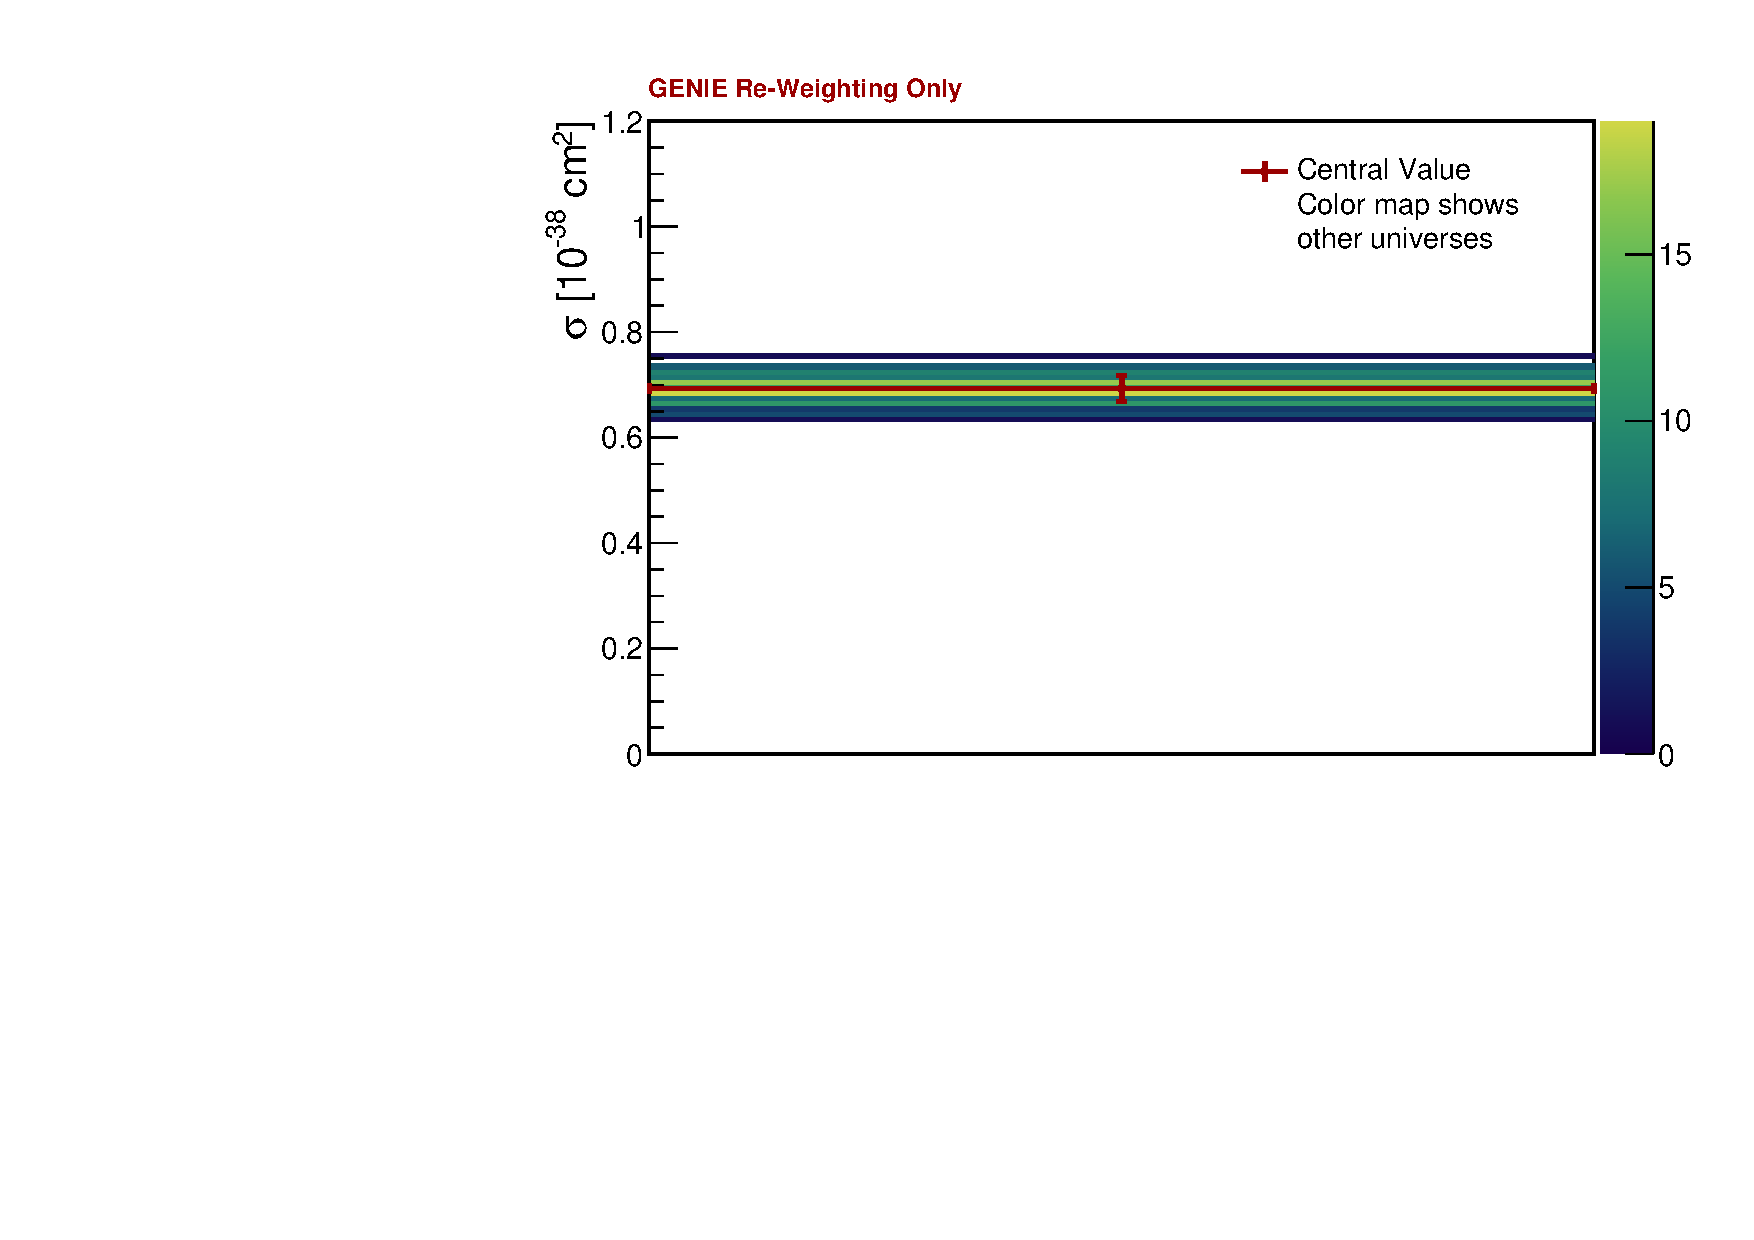
\includegraphics[width=.70\textwidth]{images/genie_covariance_plots/genie_multisim_onebin_xsec_all_fancy}
\caption[Cross-Section Modelling Uncertainties - Total Cross Section]{\emph{Cross-Section Modelling Uncertainties.} Total data extracted cross sections for all the simulated universes in the colour map. The red graph shows the total data extracted cross section for the nominal \acrshort{mc}. The red vertical bars show the \g systematic uncertainty derived from the \emph{multisims} according to Equation~\eqref{eq:cov_syst_uni}. The relative systematic uncertainty on the total cross section is 3.55\%.}
\label{fig:genie_multisim_onebin}
\end{figure}

The relative uncertainty on the total cross section due to the \g variations amounts to $3.55\%$. 
Figure~\ref{fig:genie_multisim_mumom_cov_matrix_2d} and \ref{fig:genie_multisim_muangle_xsec_all_fancy} show the covariance matrices for the muon momentum and $\cos\theta$ cross sections, respectively. In the same figures, the covariance and fractional covariance matrices, as well as the correlation matrices, all calculated according to Equations~\eqref{eq:cov_syst_uni},~\eqref{eq:cov_frac} and~\eqref{eq:corr} are shown as well.

\begin{figure}[t]
%\begin{adjustwidth}{-1cm}{-1cm}
\centering
\subfloat[][Data extracted cross sections.]
   {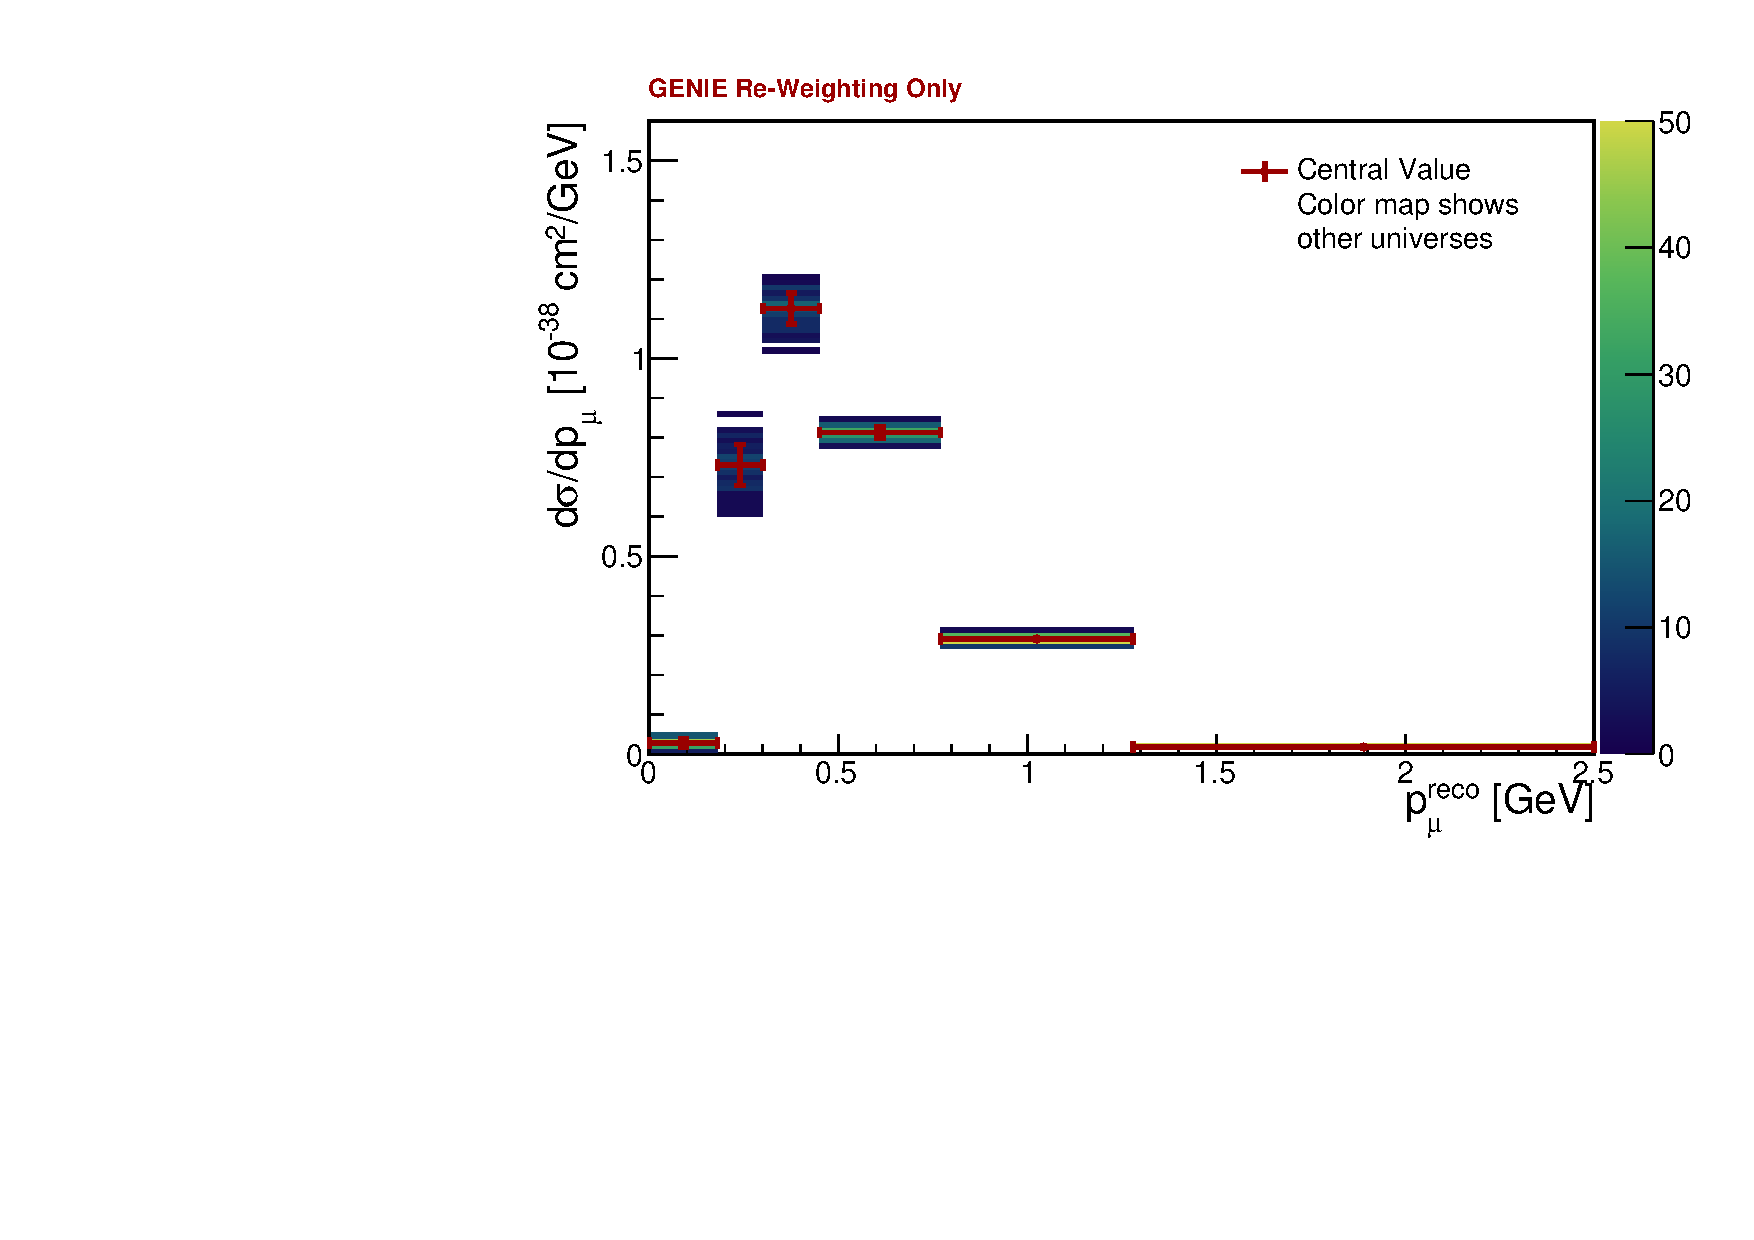
\includegraphics[width=.5\textwidth]{images/genie_covariance_plots/genie_multisim_mumom_xsec_all_fancy}
   \label{fig:genie_multisim_mumom_xsec_all_fancy}} 
\subfloat[][Covariance matrix.]
   {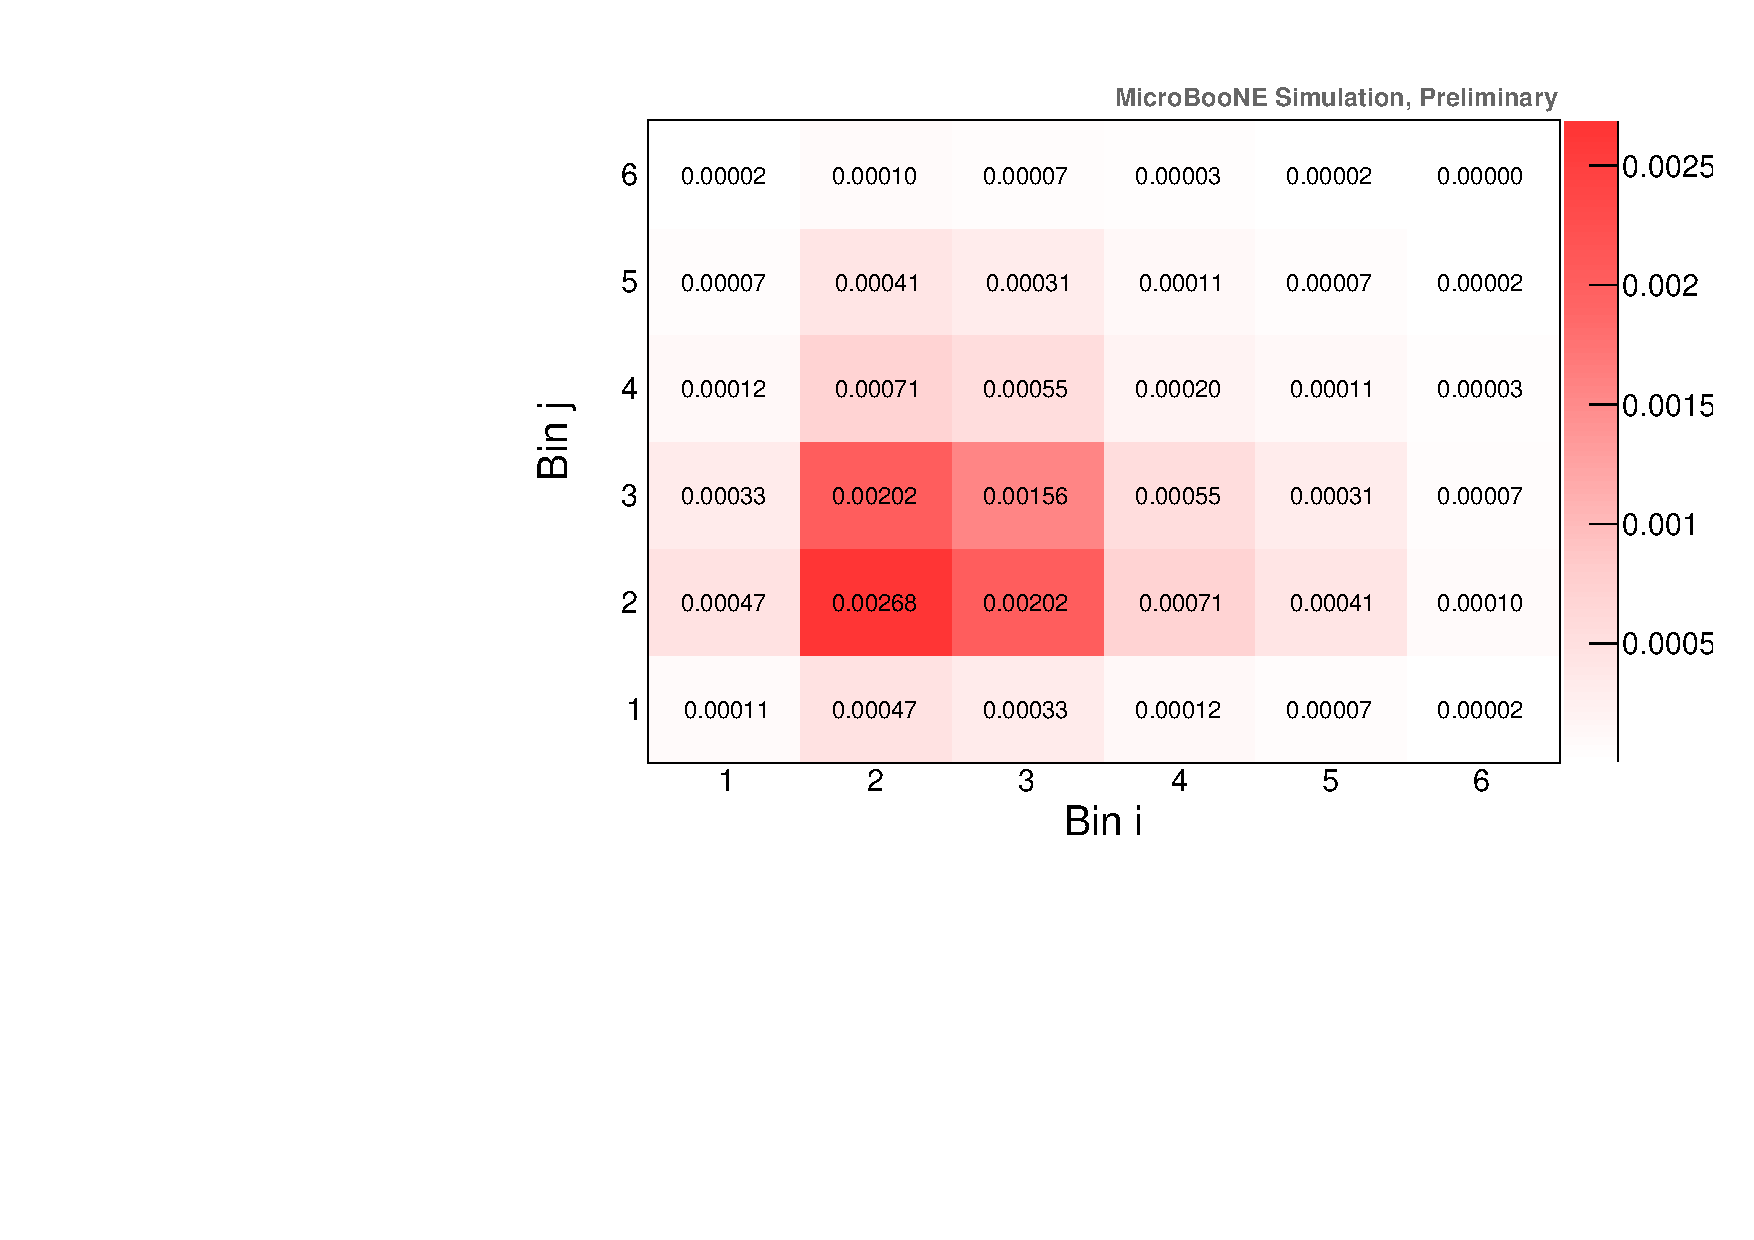
\includegraphics[width=.5\textwidth]{images/genie_covariance_plots/genie_multisim_mumom_cov_matrix_2d}
   \label{fig:genie_multisim_mumom_cov_matrix_2d}} \\
\subfloat[][Fractional covariance matrix.]
   {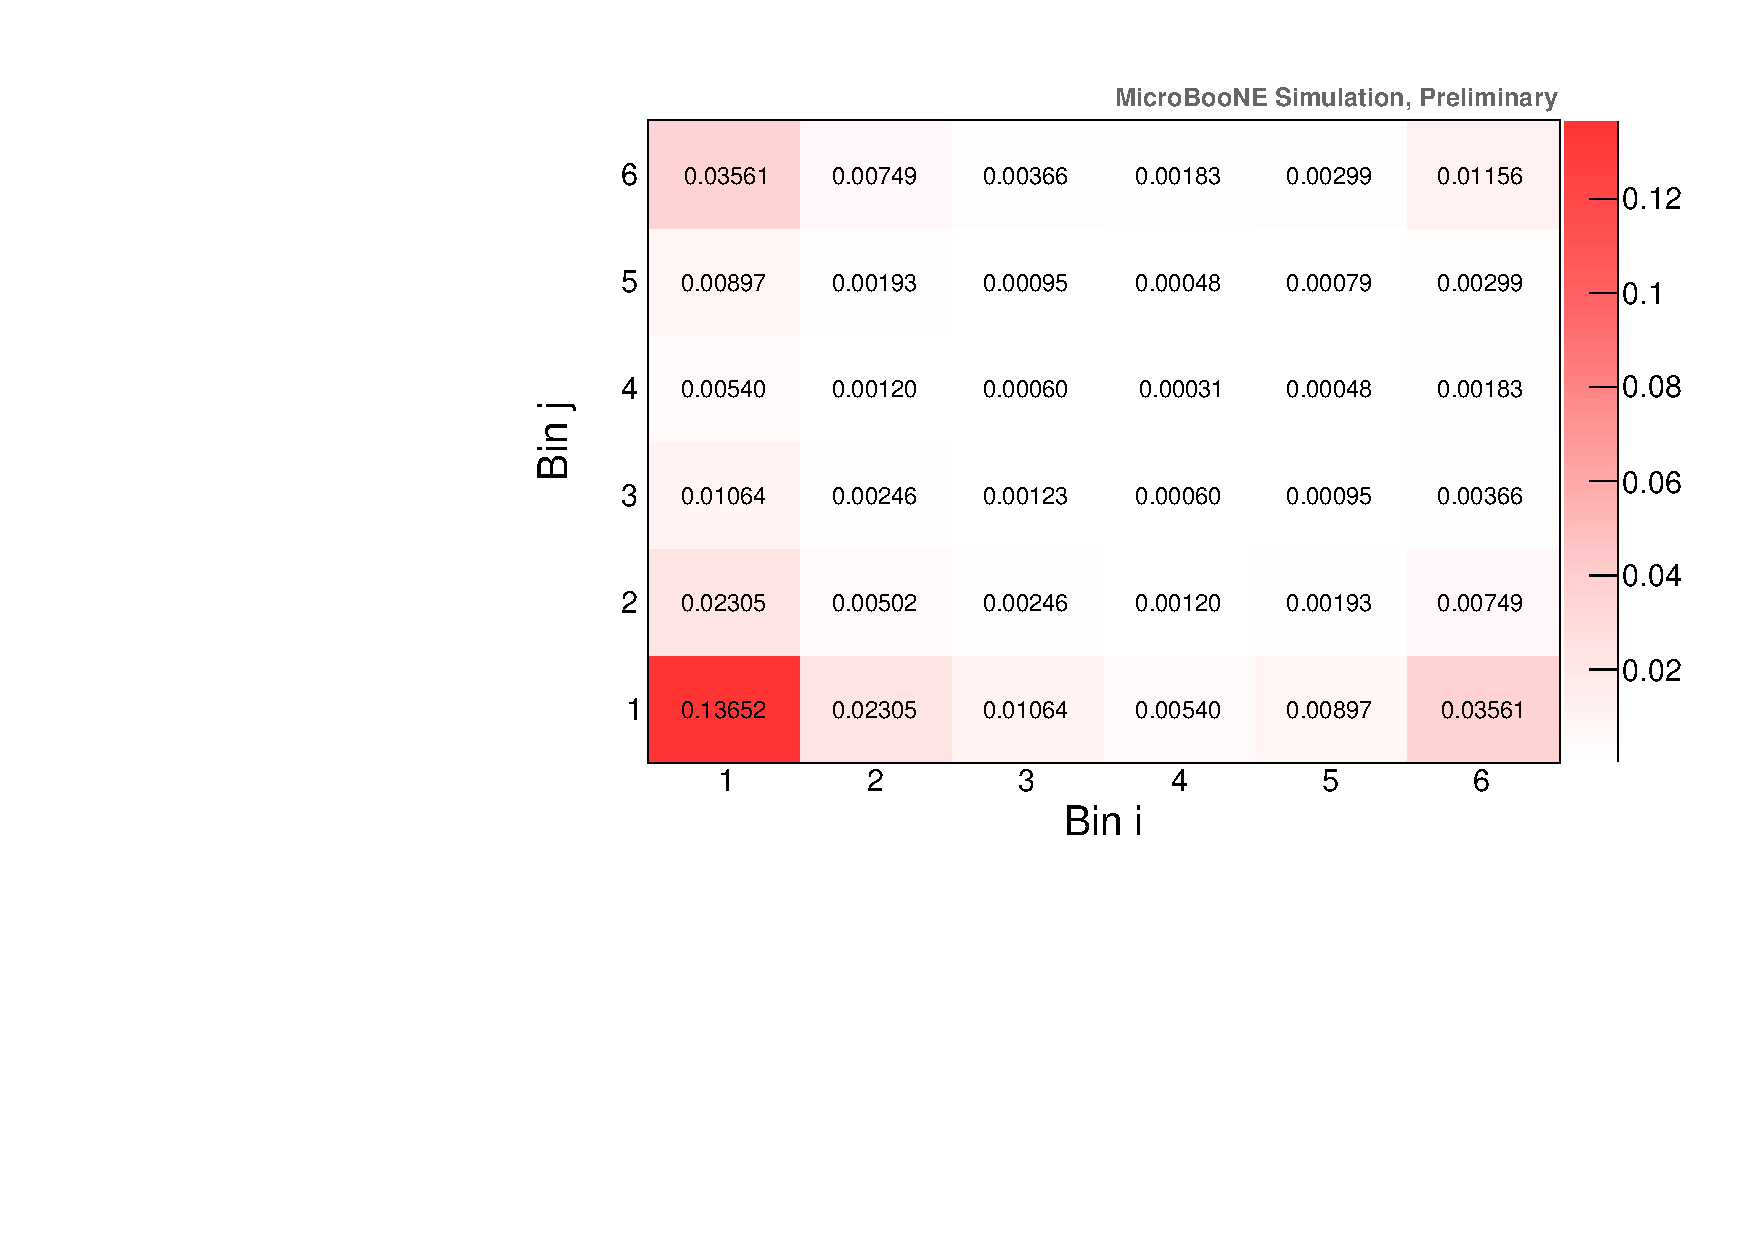
\includegraphics[width=.5\textwidth]{images/genie_covariance_plots/genie_multisim_mumom_cov_frac_matrix_2d}
   \label{fig:genie_multisim_mumom_cov_frac_matrix_2d}} 
\subfloat[][Correlation matrix.]
   {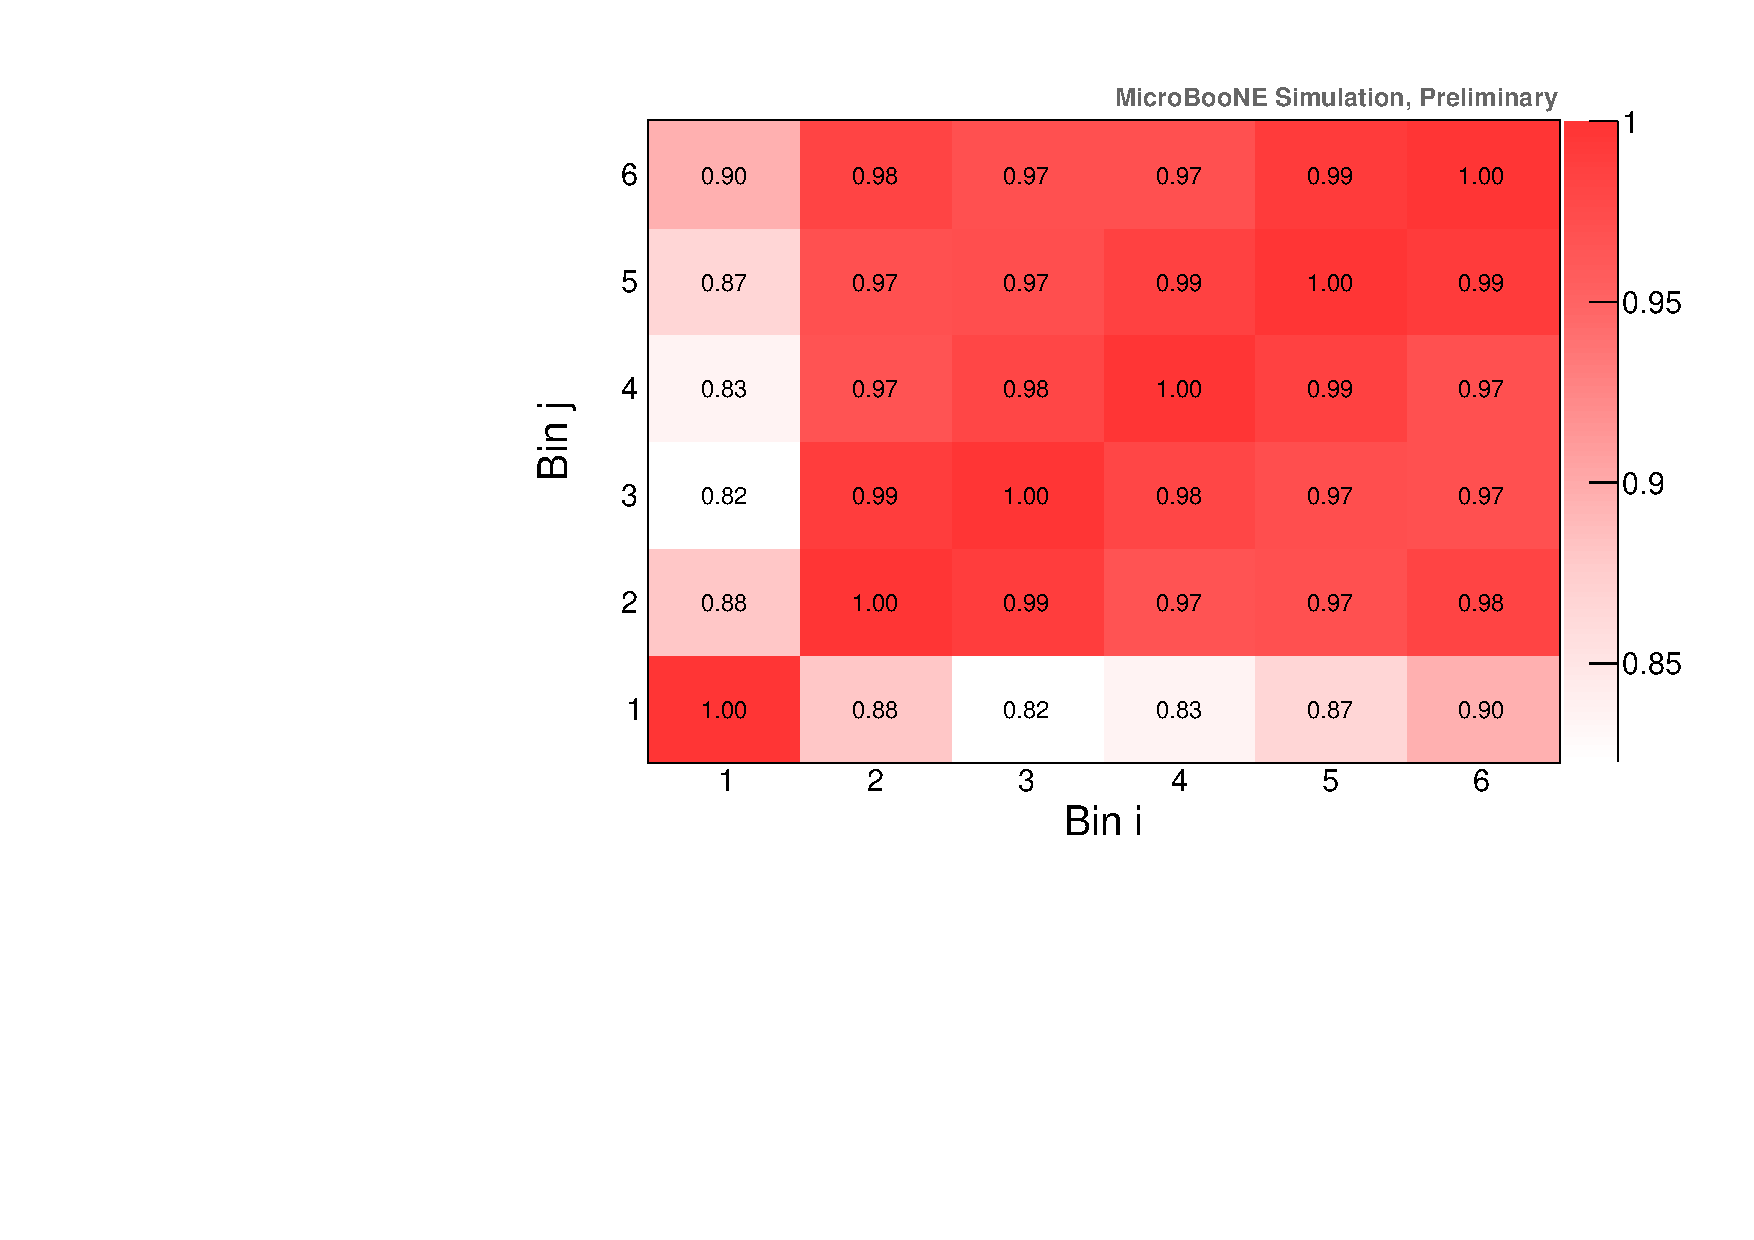
\includegraphics[width=.5\textwidth]{images/genie_covariance_plots/genie_multisim_mumom_corr_matrix_2d}
   \label{fig:genie_multisim_mumom_corr_matrix_2d}} \\
\caption[Cross-Section Modelling Uncertainties - Cross Section in $p_\mu$]{\emph{Cross-Section Modelling Uncertainties.} \protect\subref{fig:genie_multisim_mumom_xsec_all_fancy}: data extracted differential cross section in muon momentum for all the simulated universes in the colour map. The red graph shows the data extracted cross section for the nominal \acrshort{mc}. The red vertical bars show the \g systematic uncertainties derived from the \emph{multisims} according to Equation~\eqref{eq:cov_syst_uni}. \protect\subref{fig:genie_multisim_mumom_cov_matrix_2d}, ~\protect\subref{fig:genie_multisim_mumom_cov_frac_matrix_2d} and ~\protect\subref{fig:genie_multisim_mumom_corr_matrix_2d}: covariance, fractional covariance, and  correlation matrices, respectively.}
\label{fig:genie_multisim_mumom}
%\end{adjustwidth}
\end{figure}

\begin{figure}[t]
%\begin{adjustwidth}{-1cm}{-1cm}
\centering
\subfloat[][Data extracted cross sections.]
   {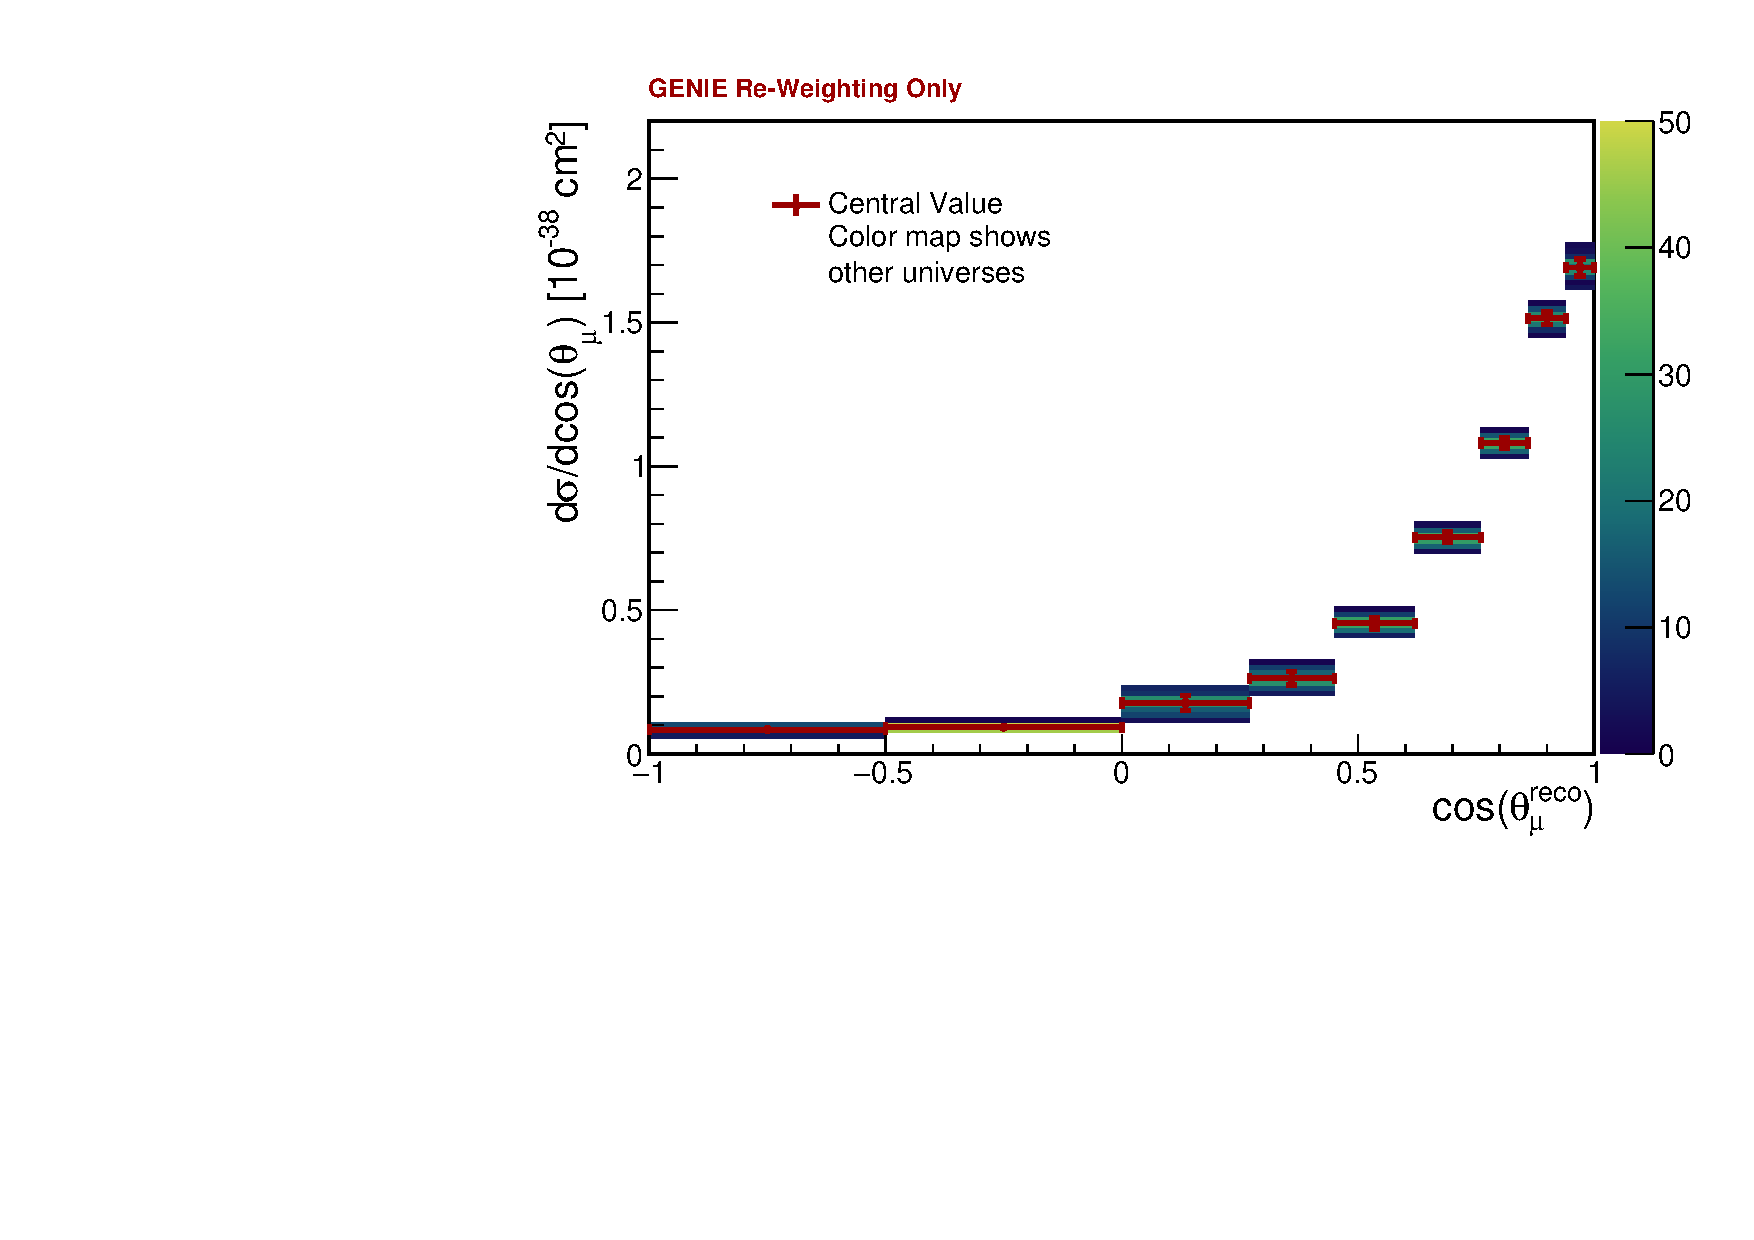
\includegraphics[width=.5\textwidth]{images/genie_covariance_plots/genie_multisim_muangle_xsec_all_fancy}
   \label{fig:genie_multisim_muangle_xsec_all_fancy}} 
\subfloat[][Covariance matrix.]
   {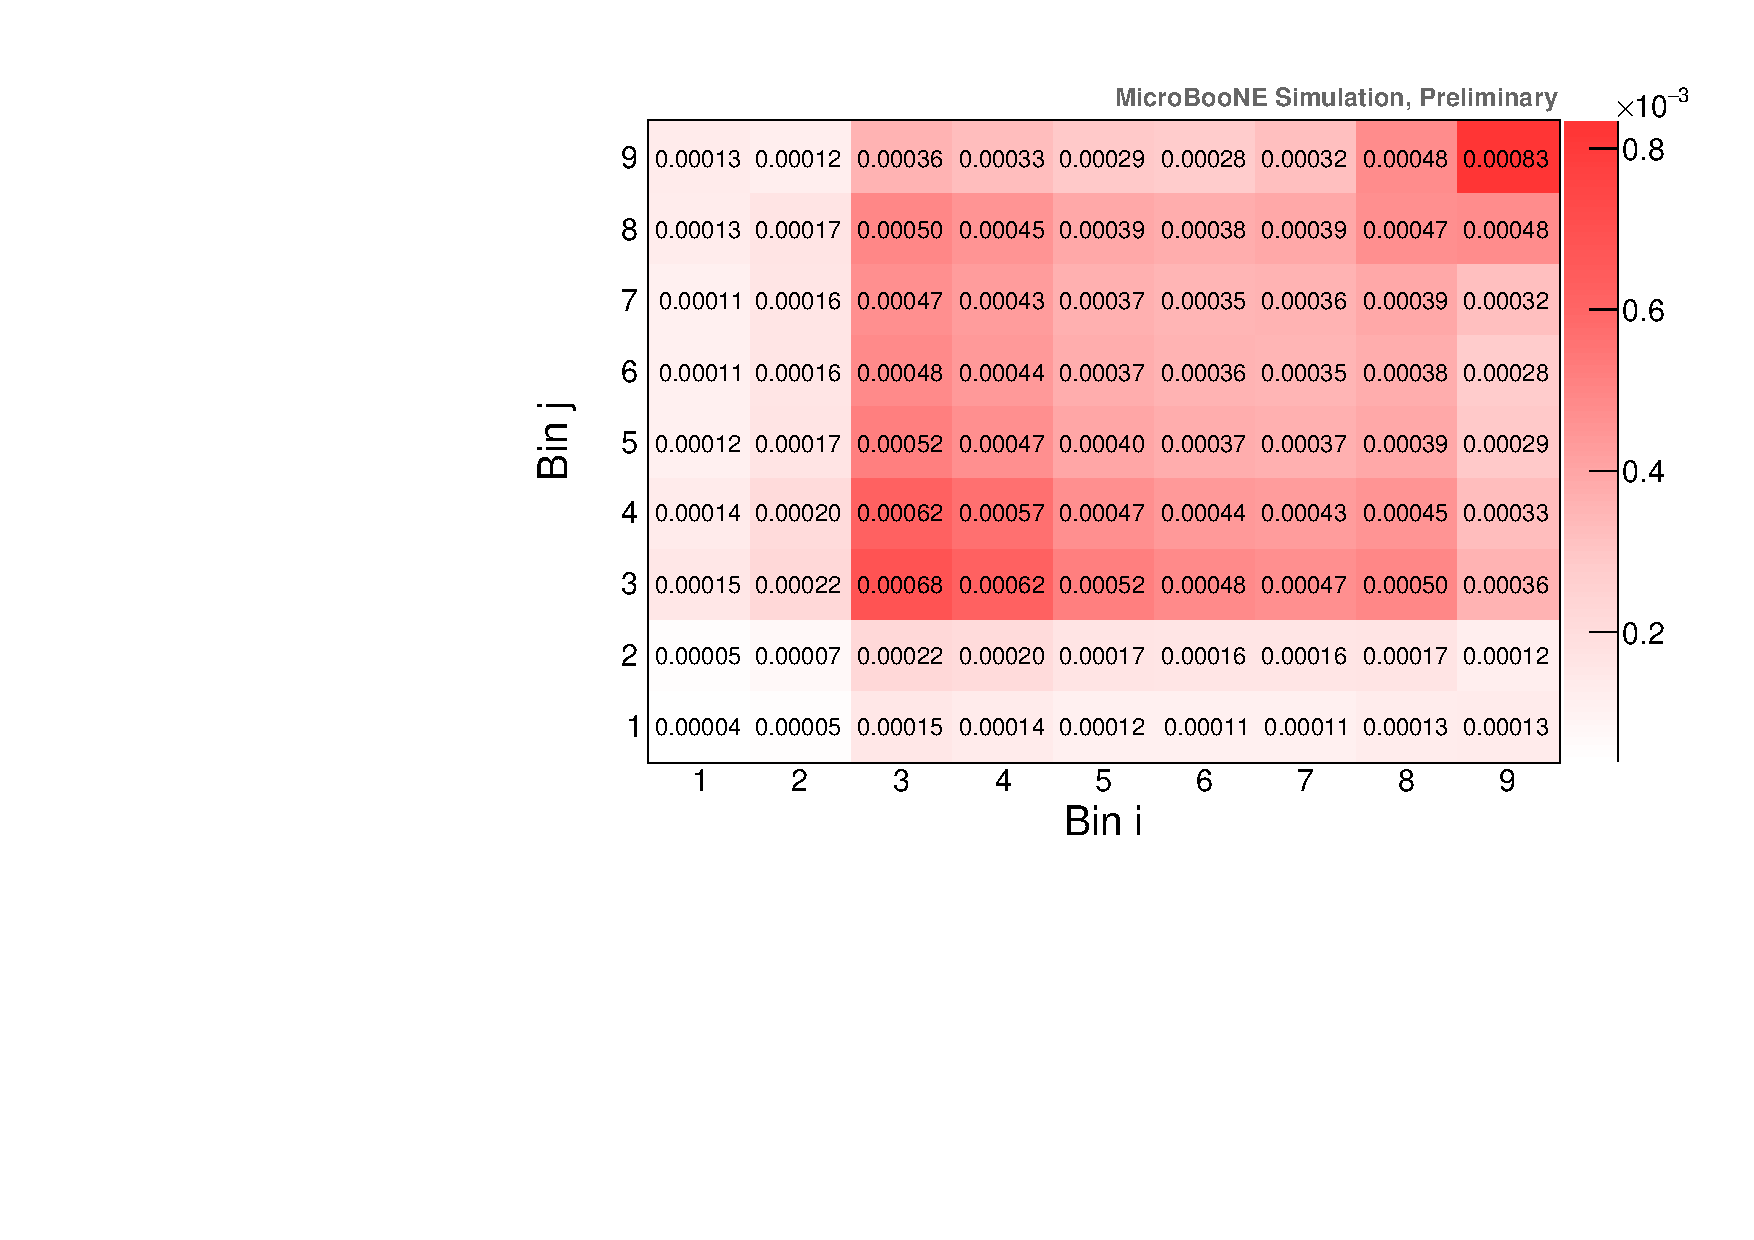
\includegraphics[width=.5\textwidth]{images/genie_covariance_plots/genie_multisim_muangle_cov_matrix_2d}
   \label{fig:genie_multisim_muangle_cov_matrix_2d}} \\
\subfloat[][Fractional covariance matrix.]
   {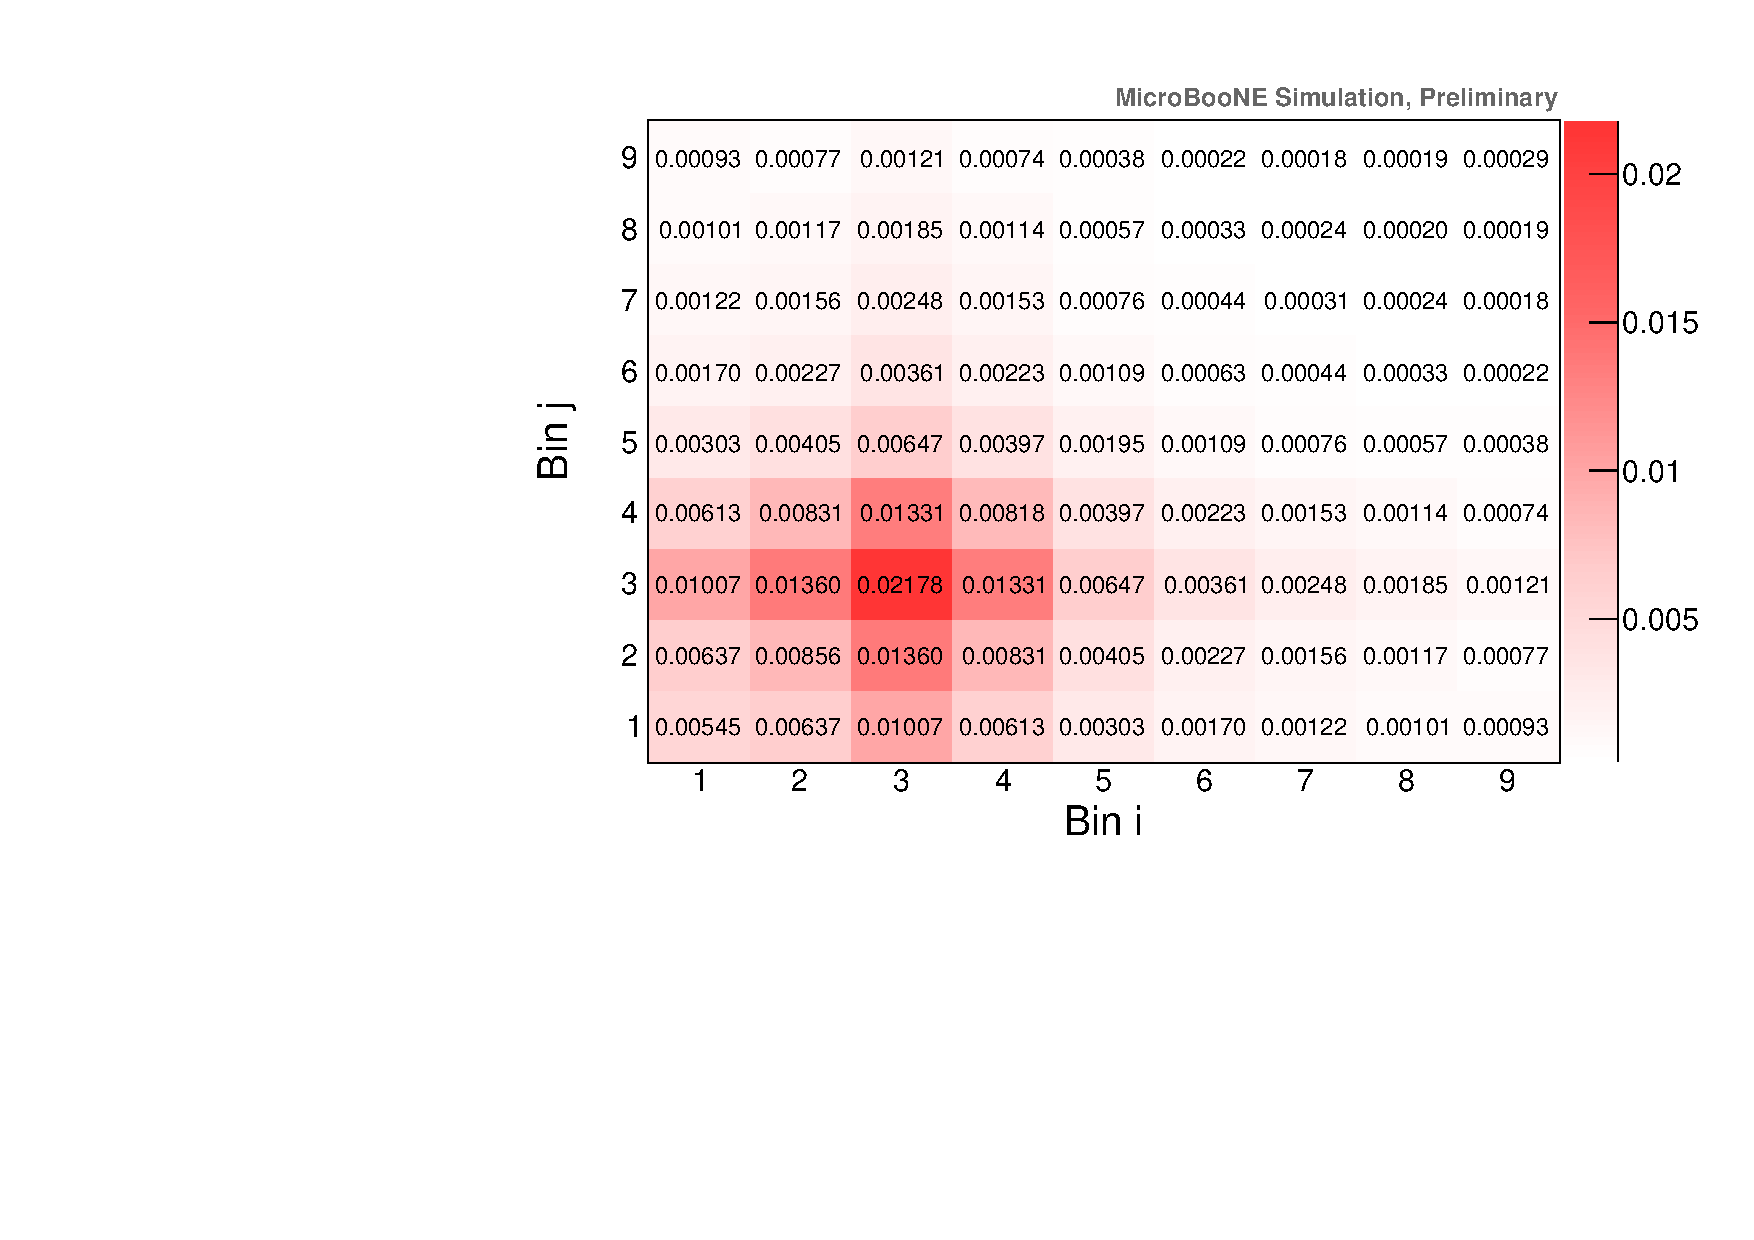
\includegraphics[width=.5\textwidth]{images/genie_covariance_plots/genie_multisim_muangle_cov_frac_matrix_2d}
   \label{fig:genie_multisim_muangle_cov_frac_matrix_2d}}
\subfloat[][Correlation matrix.]
   {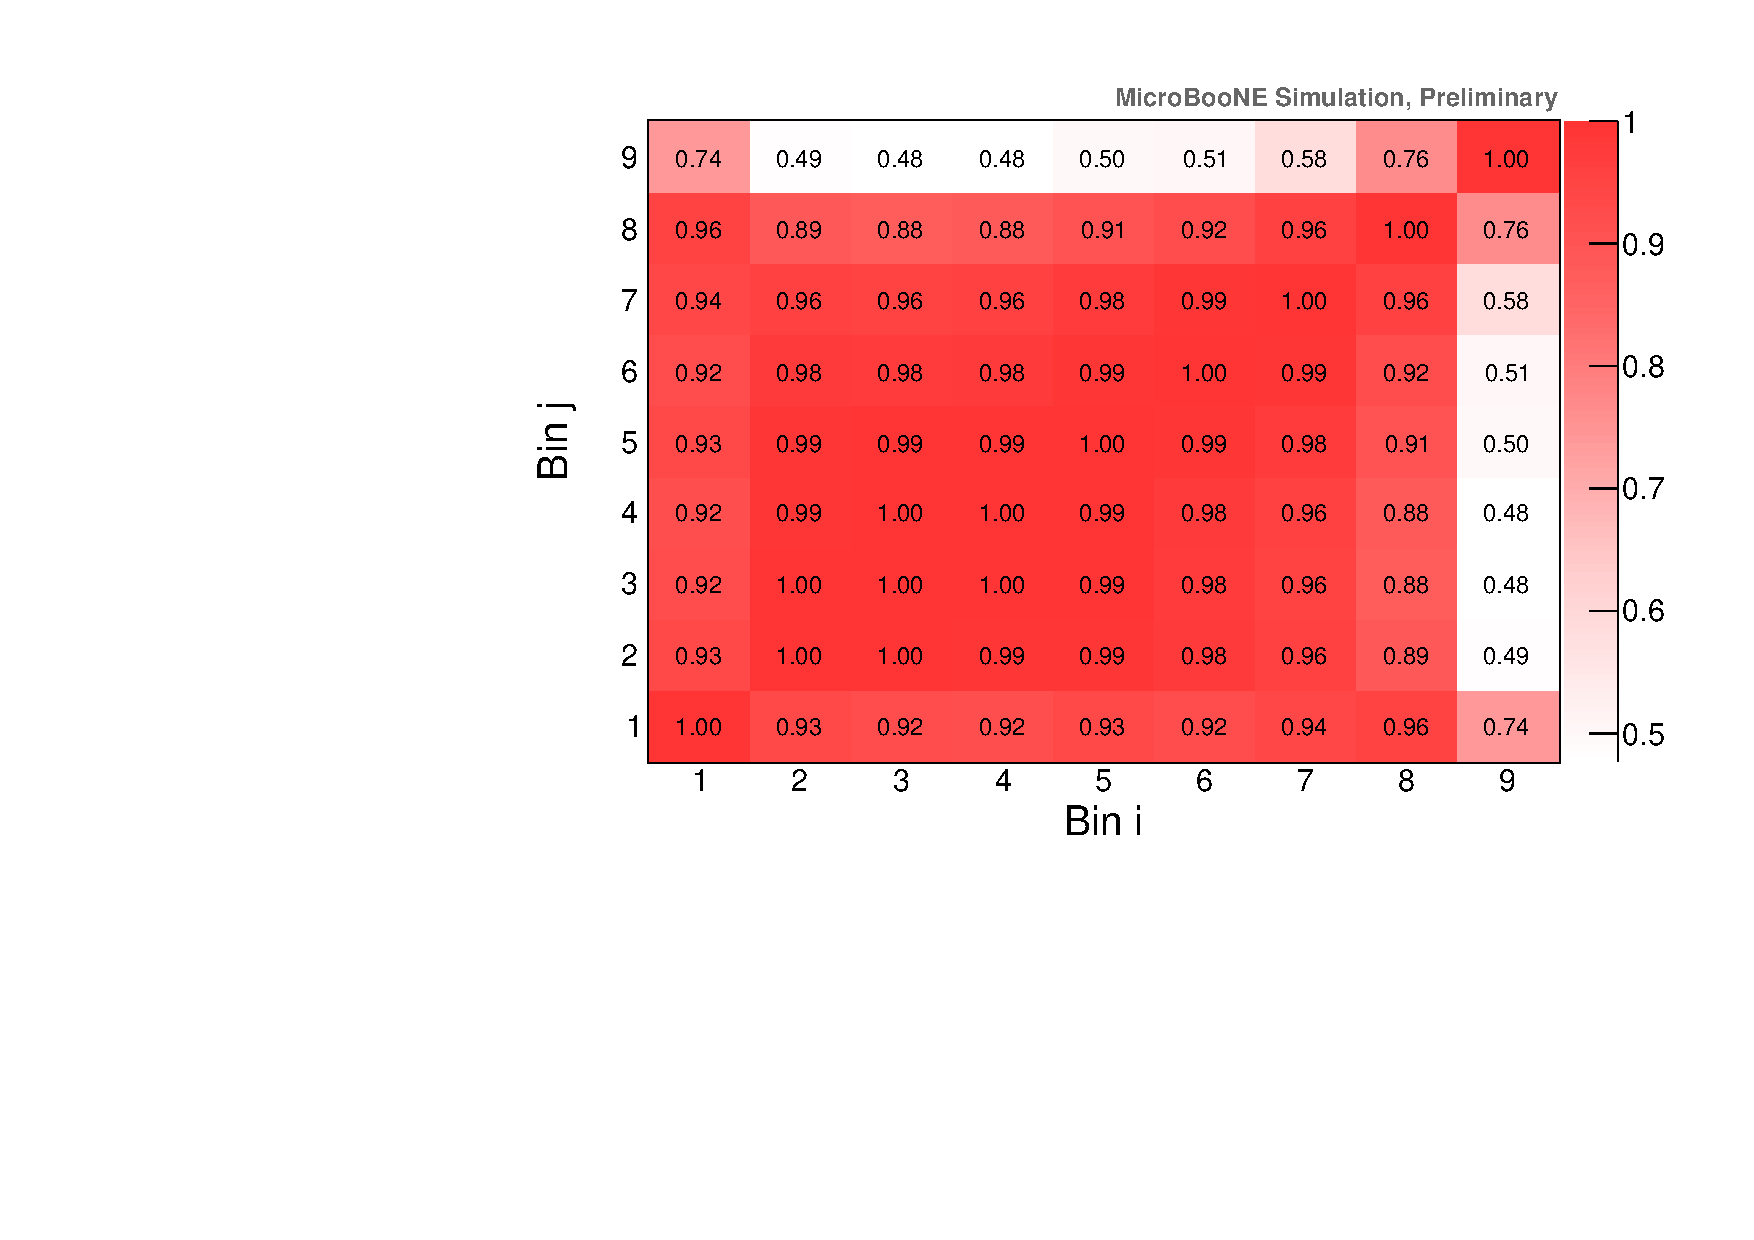
\includegraphics[width=.5\textwidth]{images/genie_covariance_plots/genie_multisim_muangle_corr_matrix_2d}
   \label{fig:genie_multisim_muangle_corr_matrix_2d}} \\
\caption[Cross-Section Modelling Uncertainties - Cross Section in $\cos\theta_\mu$]{\emph{Cross-Section Modelling Uncertainties.} \protect\subref{fig:genie_multisim_muangle_xsec_all_fancy}: data extracted differential cross section in muon angle for all the simulated universes in the colour map. The red graph shows  the data extracted cross section for the nominal \acrshort{mc}. The red vertical bars show the \g systematic uncertainties derived from the \emph{multisims} according to Equation~\eqref{eq:cov_syst_uni}.  \protect\subref{fig:genie_multisim_muangle_cov_matrix_2d}, \protect\subref{fig:genie_multisim_muangle_cov_frac_matrix_2d} and \protect\subref{fig:genie_multisim_muangle_corr_matrix_2d}: covariance, fractional covariance, and correlation matrices, respectively.}
\label{fig:genie_multisim_muangle}
%\end{adjustwidth}
\end{figure}


In the same way, the reweighting is performed with the double-differential cross section, for which all the universes are shown in Figure~\ref{fig:genie_multisim_muangle_mumom_xsec_all_fancy_2d}. Here, all the extracted cross sections are displayed with a green line, and the central value cross section is in red. The covariance matrix is also shown in Figure~\ref{fig:genie_multisim_muangle_mumom_cov_matrix_2d}.

\begin{figure}[]
\centering
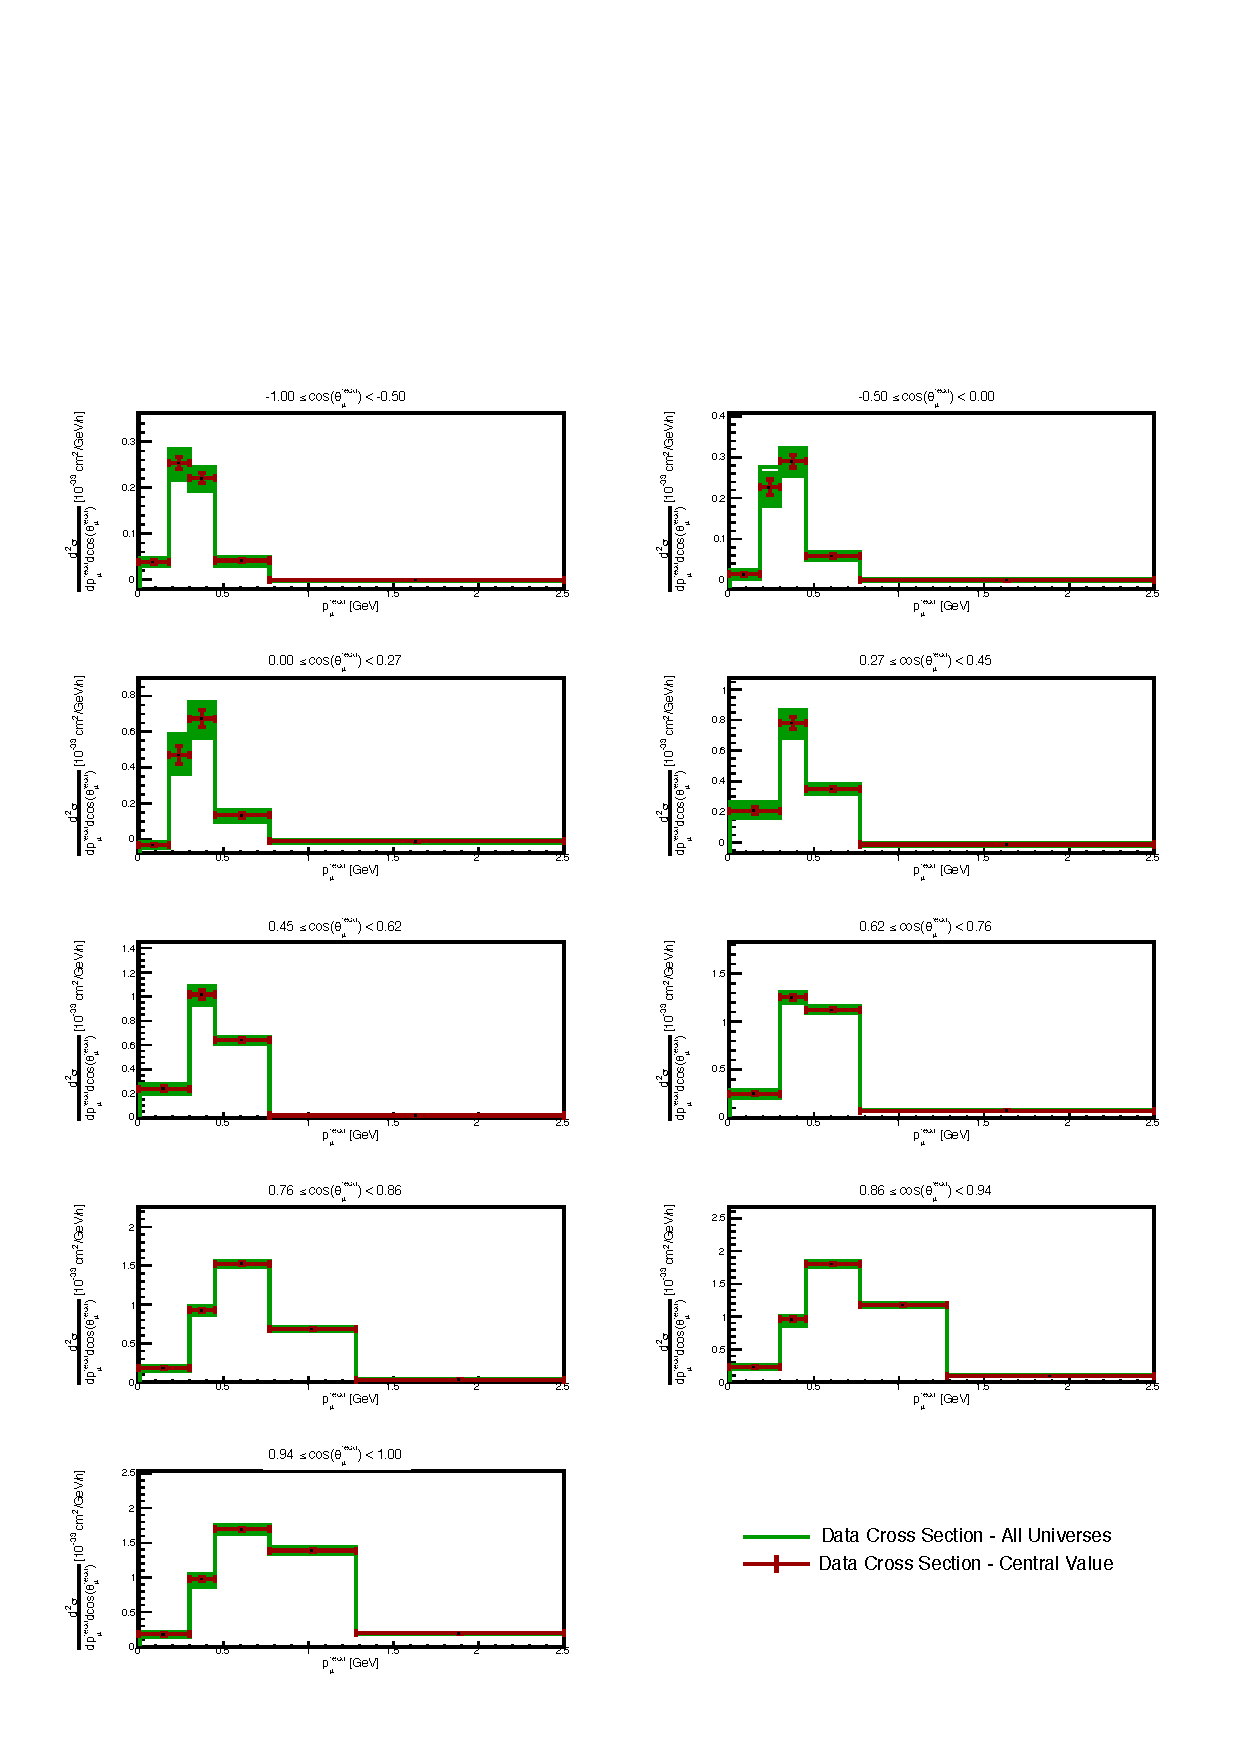
\includegraphics[width=1.0\textwidth]{images/genie_covariance_plots/genie_multisim_muangle_mumom_xsec_all_fancy_2d}
\caption[Cross-Section Modelling Uncertainties - Double-Differential Cross Section - Universes Distributions]{\emph{Cross-Section Modelling Uncertainties.} Data extracted cross sections for every universe. The green cross sections show the 100 \g universes, while the red cross section shows the central value. The vertical vertical bars show the standard deviation of all the universes with respect to the central value (i.e. the systematic uncertainty).}
\label{fig:genie_multisim_muangle_mumom_xsec_all_fancy_2d}
\end{figure}

\begin{figure}[]
\centering
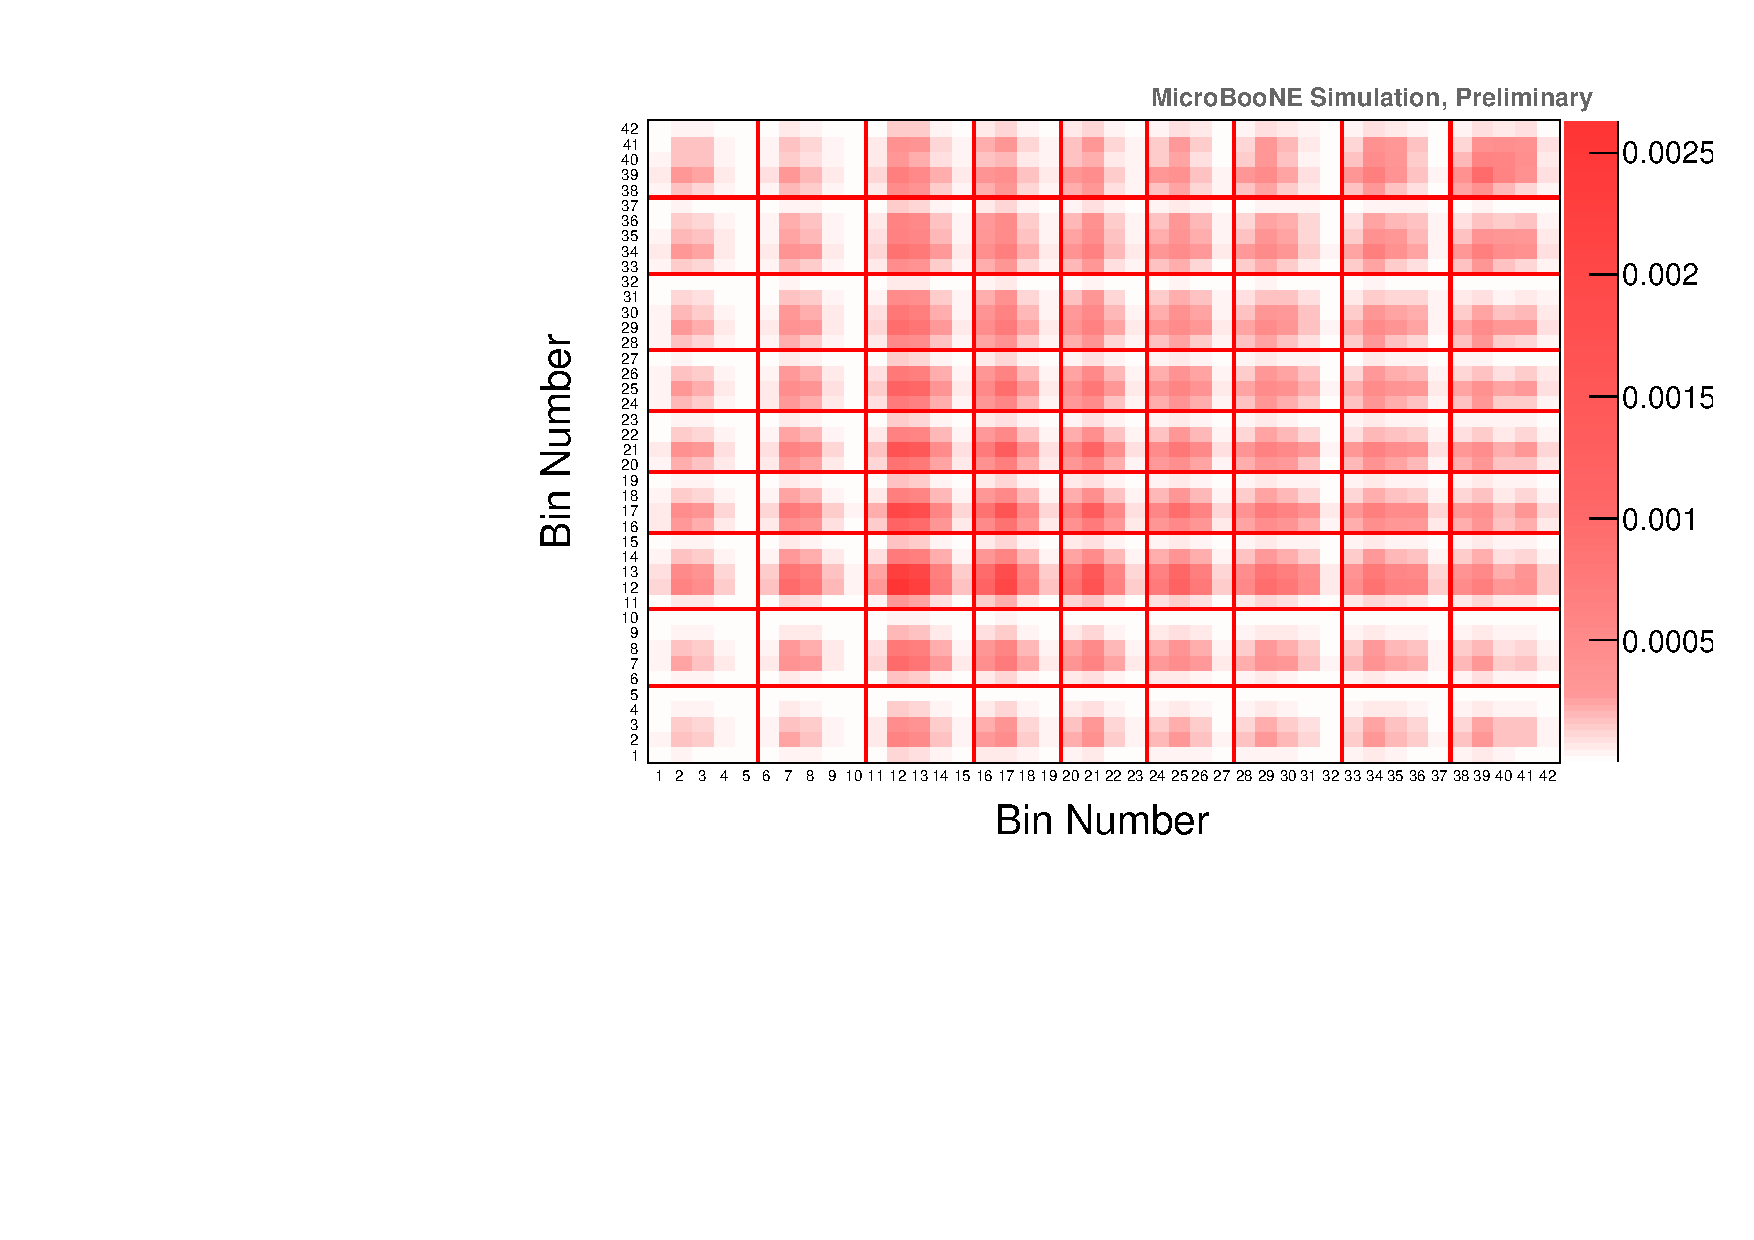
\includegraphics[width=.85\textwidth]{images/genie_covariance_plots/genie_multisim_muangle_mumom_cov_matrix_2d}
\caption[Cross-Section Modelling Uncertainties - Double-Differential Cross Section - Covariance Matrix]{\emph{Cross-Section Modelling Uncertainties.}  Cross-section modelling covariance matrix, for the double differential cross section.}
\label{fig:genie_multisim_muangle_mumom_cov_matrix_2d}
\end{figure}





\clearpage
\subsection{QE and MEC Cross Section Systematics}
\label{sec:error_qemec}

This section describes a method to account for uncertainties in the \acrshort{qe} cross section model, largely due to \acrshort{rpa} effects, and the choice of \acrshort{mec} model. As explained in Chapter~\ref{ch:neutrino_interactions}, \acrshort{rpa} refers to long
range multi-nucleon correlations which suppress the cross section at low $Q^2$, while \acrshort{mec} is related to scatters involving correlated pairs of nucleons. 
The MicroBooNE simulation uses the \g ``\tuneone'' model set (see Section~\ref{sec:simulation}). These models do not consider \acrshort{rpa}, and \acrshort{mec} is handled with an empirical model without associated uncertainties. To assess systematic uncertainties related to these two limitations, the baseline model is compared to an alternative model set (called ``\tunethree'' in Section~\ref{sec:simulation}). This uses the ``Valencia'' model for
\acrshort{qe} interactions \cite{nieves, nieves2}, which includes \acrshort{rpa} effects, and a more theory-driven \acrshort{mec} model. Ratios of the ``Valencia'' model with respect to the ``default'' model are treated in exclusive interaction channels as an uncertainty on the cross section, and a reweighing of the default \acrshort{mc} in relevant truth-level kinematic variables is performed. The cross sections for the two different models are shown in Figure~\ref{fig:mastbaum_qe_mec}.

\begin{figure}[p]
%\begin{adjustwidth}{-1cm}{-1cm}
\centering
\subfloat[][\acrshort{cc} \acrshort{qe} cross sections.]
   {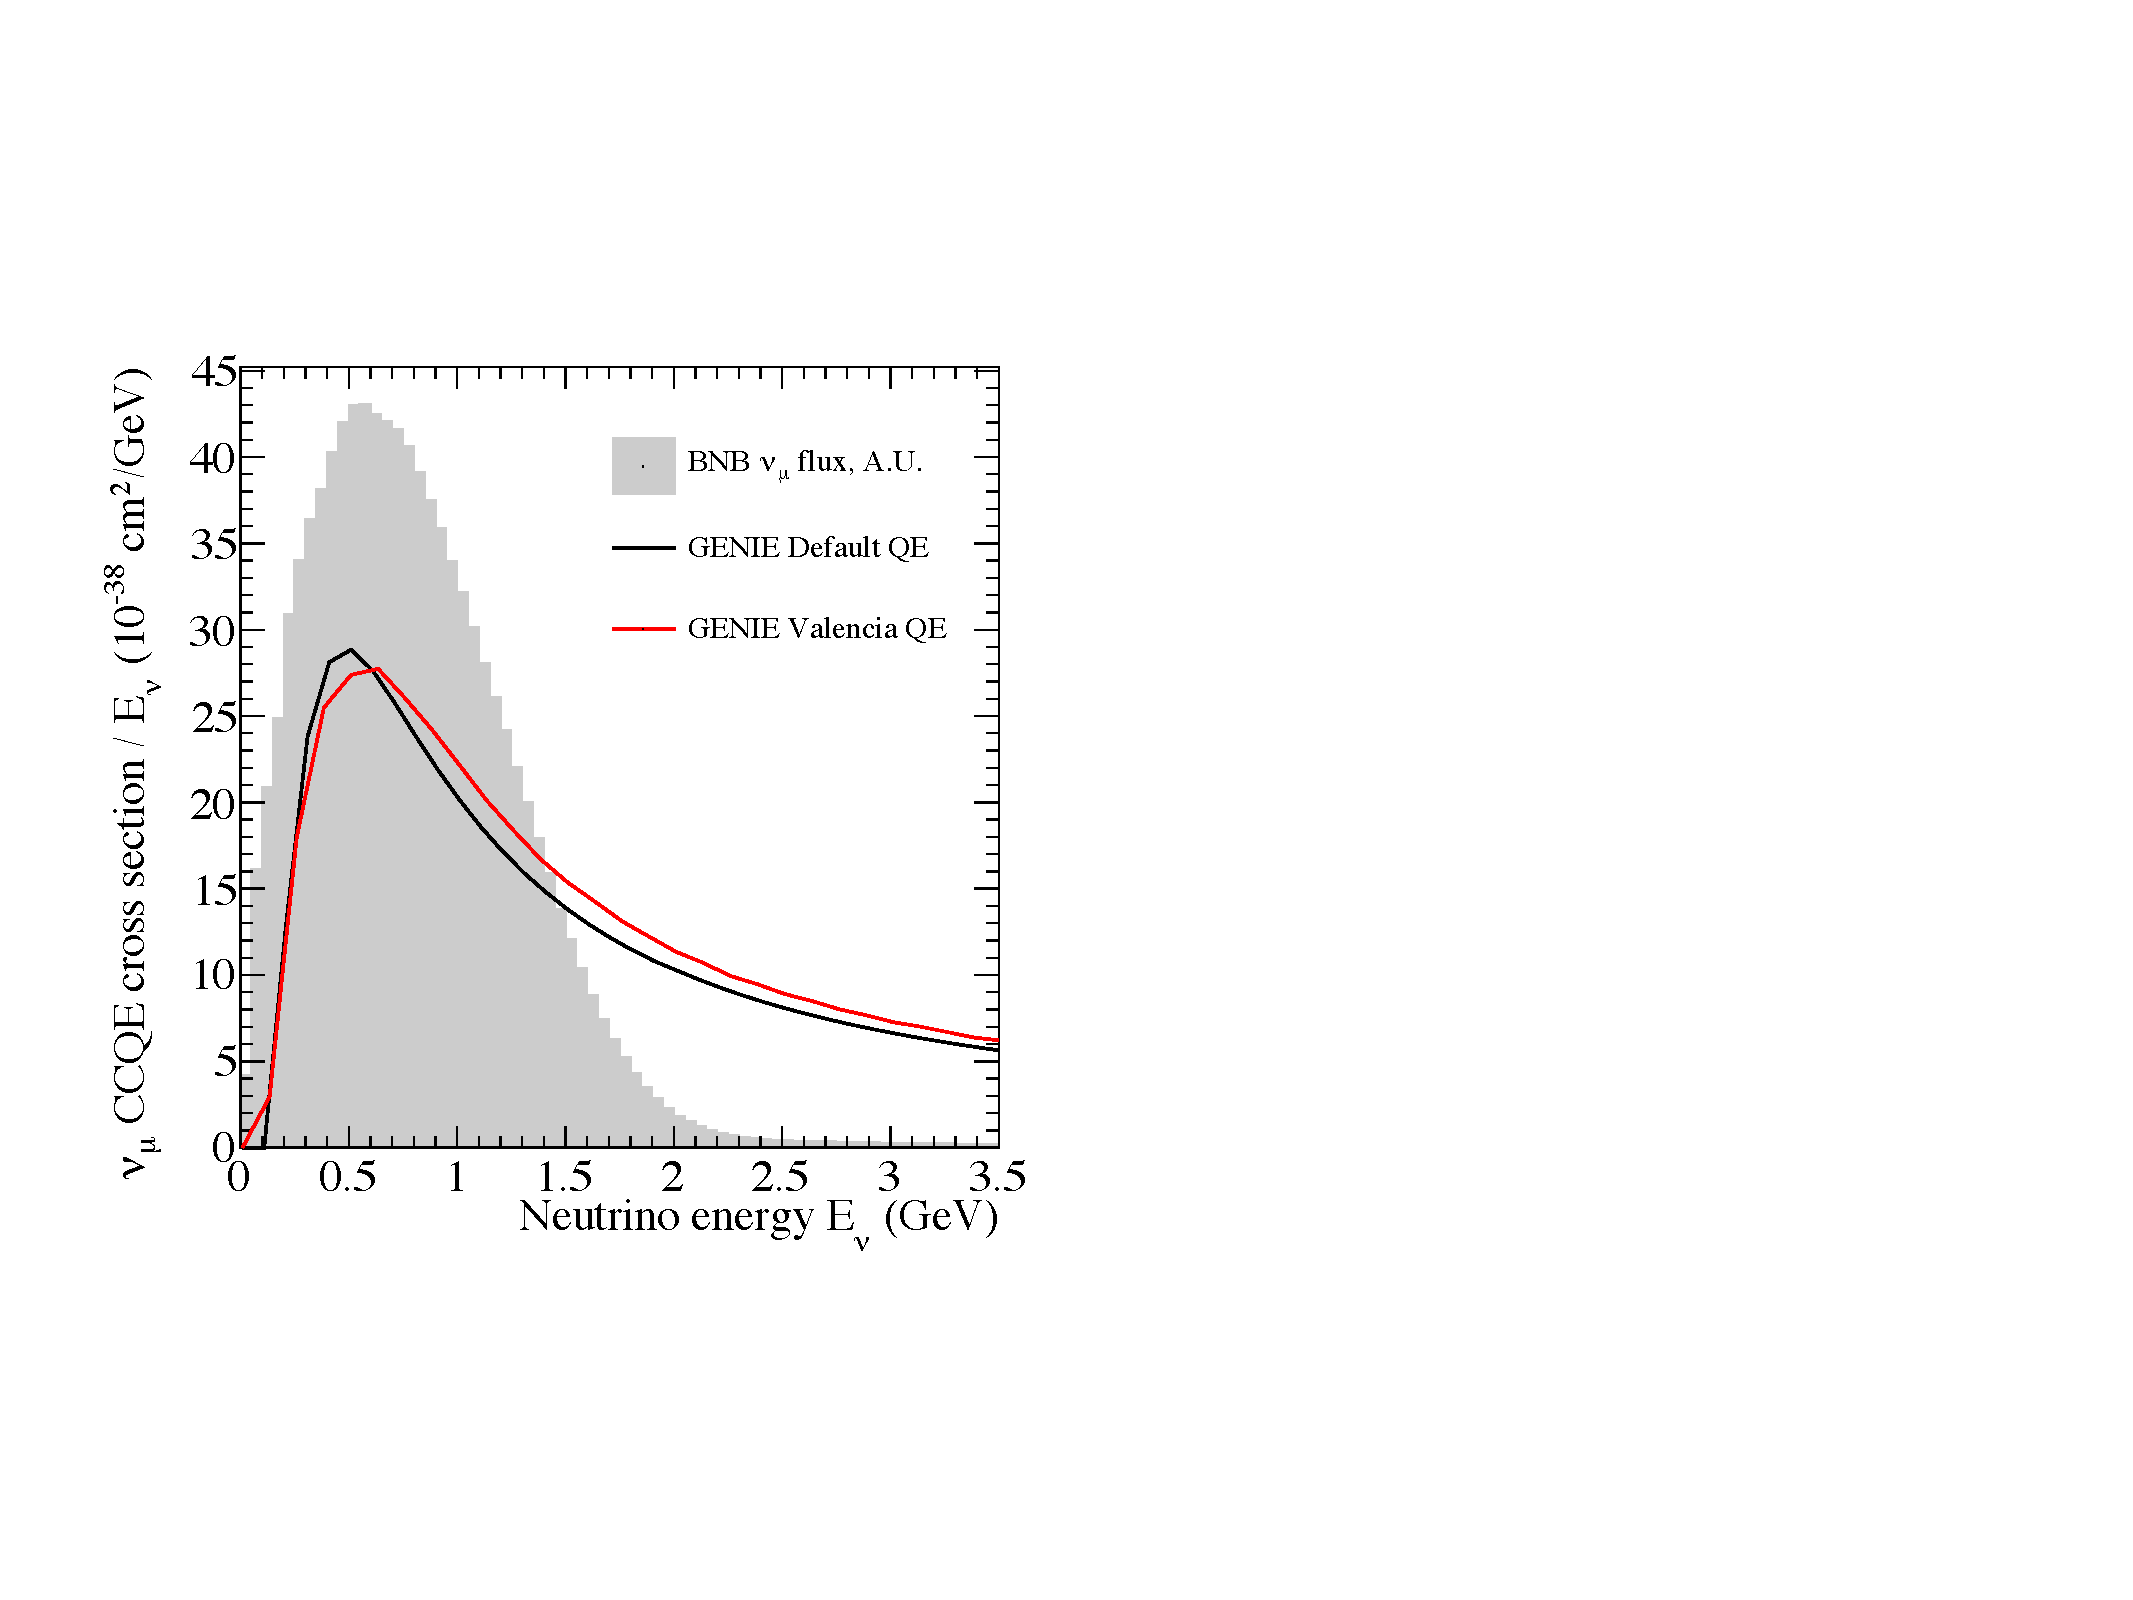
\includegraphics[width=.41\textwidth]{images/QE_MEC_Systematics/mastbaum_qe}
   \label{fig:mastbaum_qe}} \quad
\subfloat[][\acrshort{cc} \acrshort{mec} cross sections.]
   {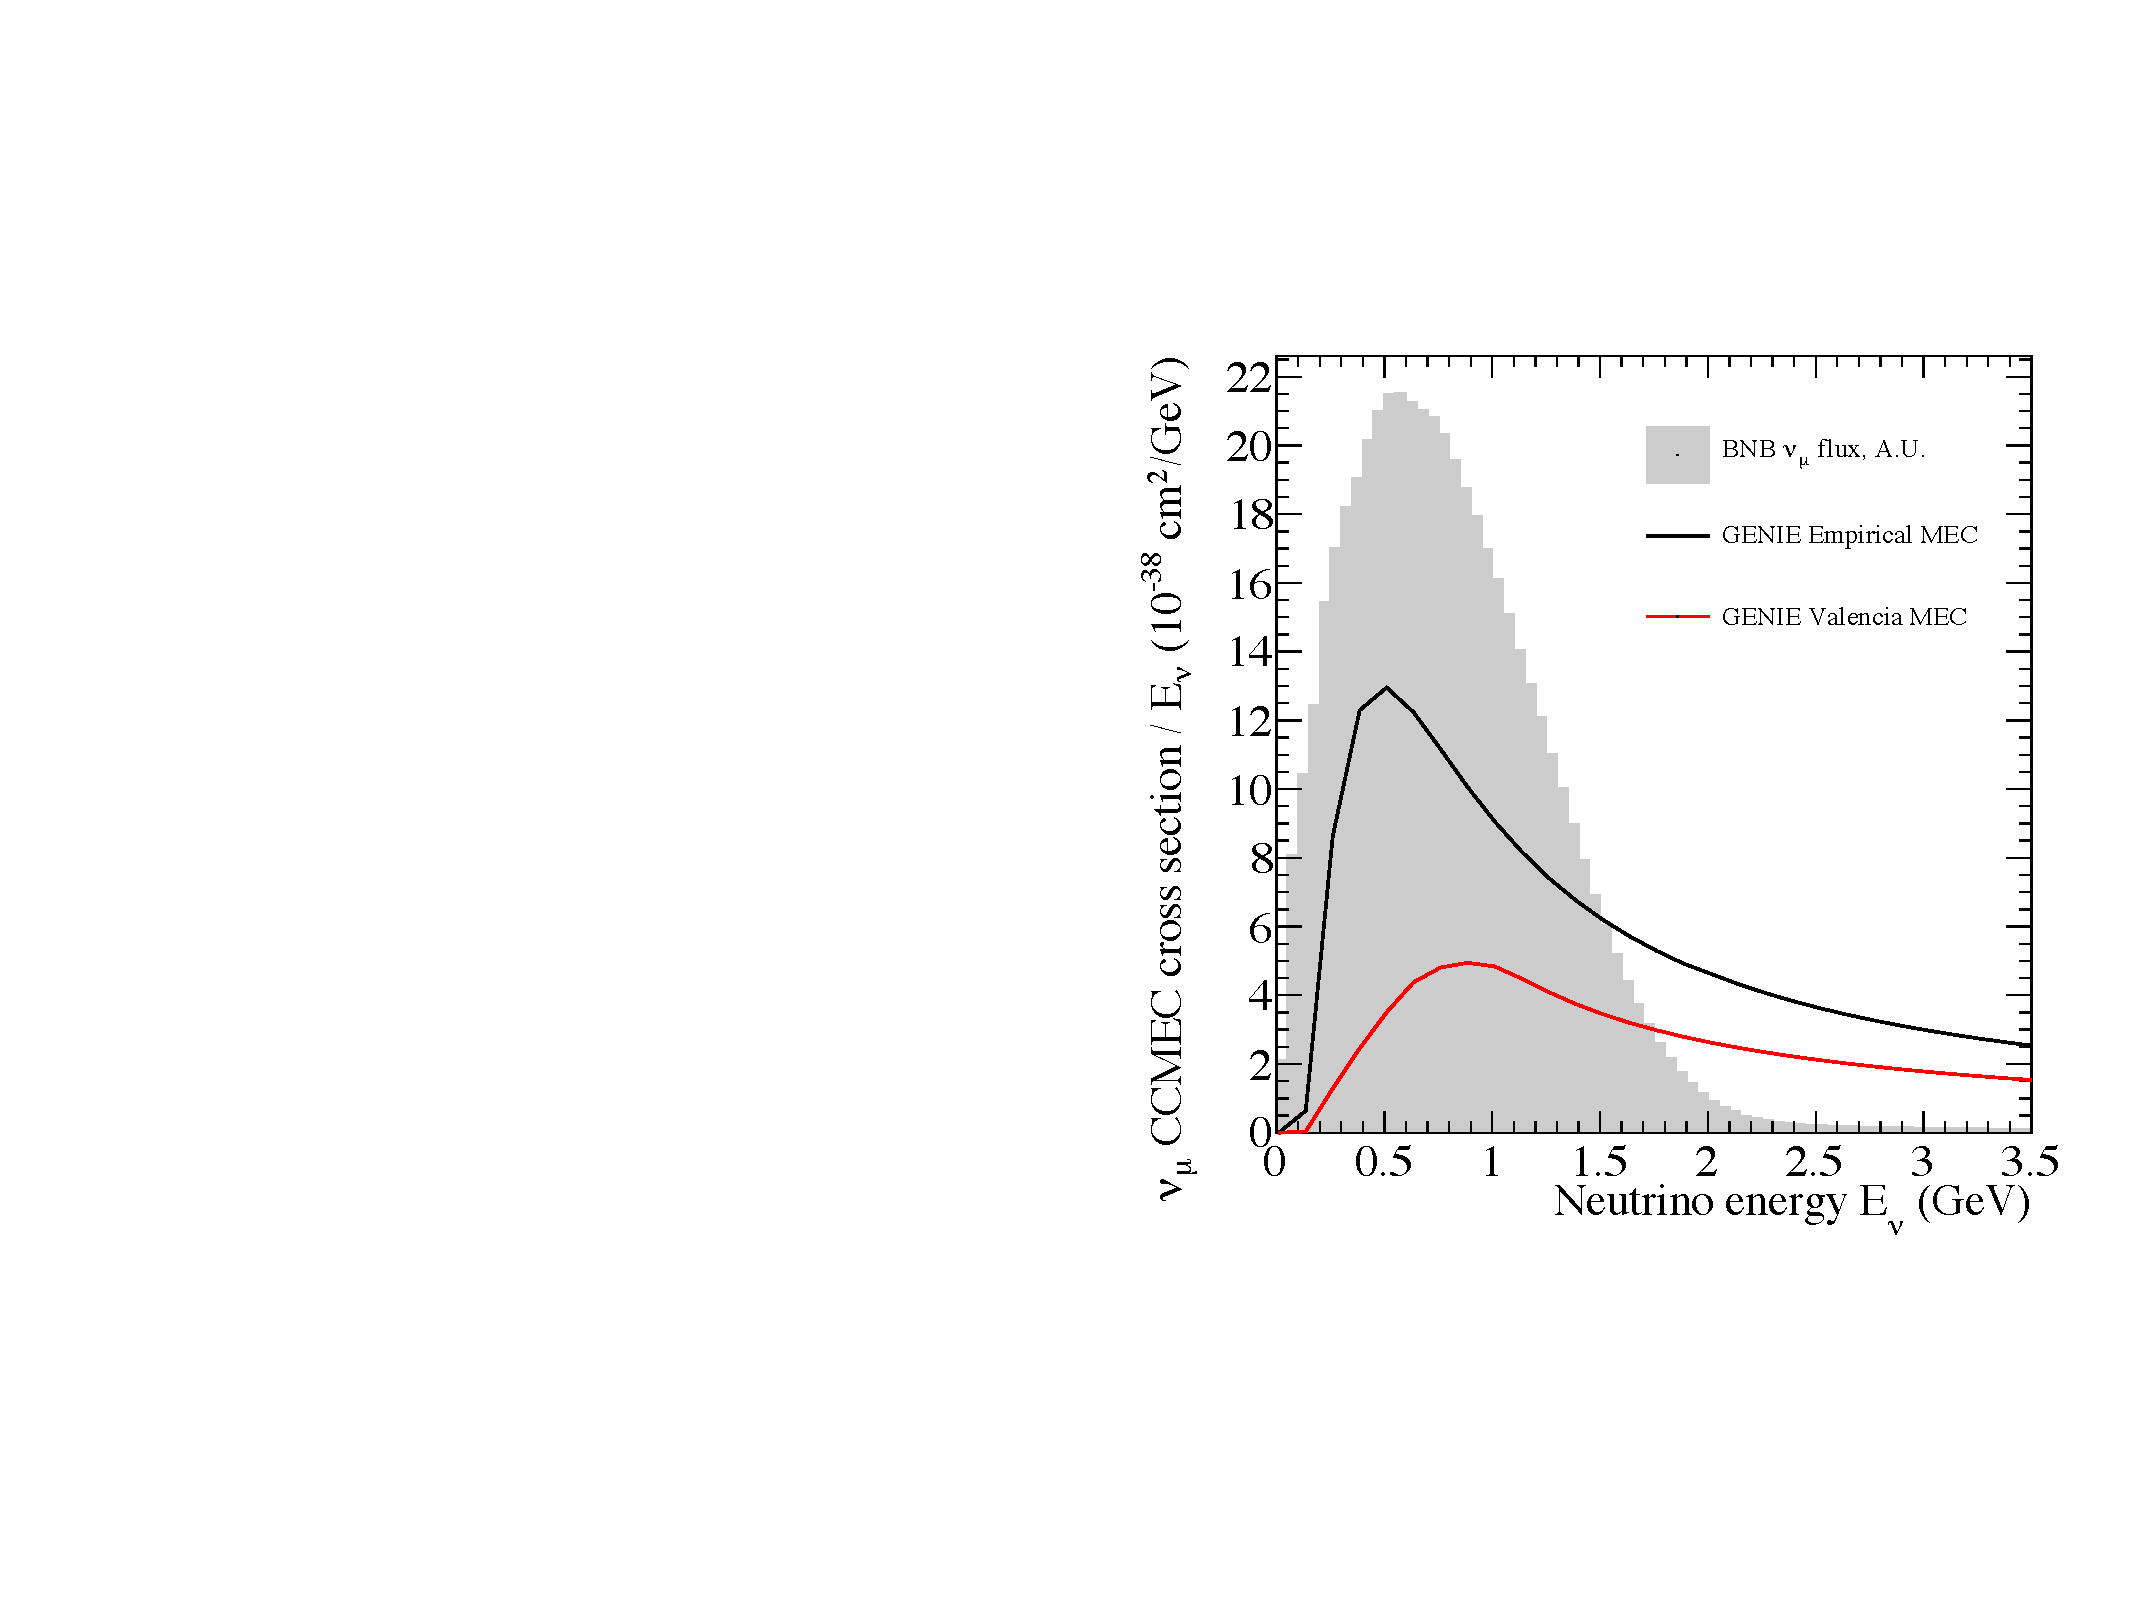
\includegraphics[width=.40\textwidth]{images/QE_MEC_Systematics/mastbaum_mec}
   \label{fig:mastbaum_mec}} \\
\subfloat[][Default model, kinematics of \acrshort{cc} \acrshort{qe} events.]
   {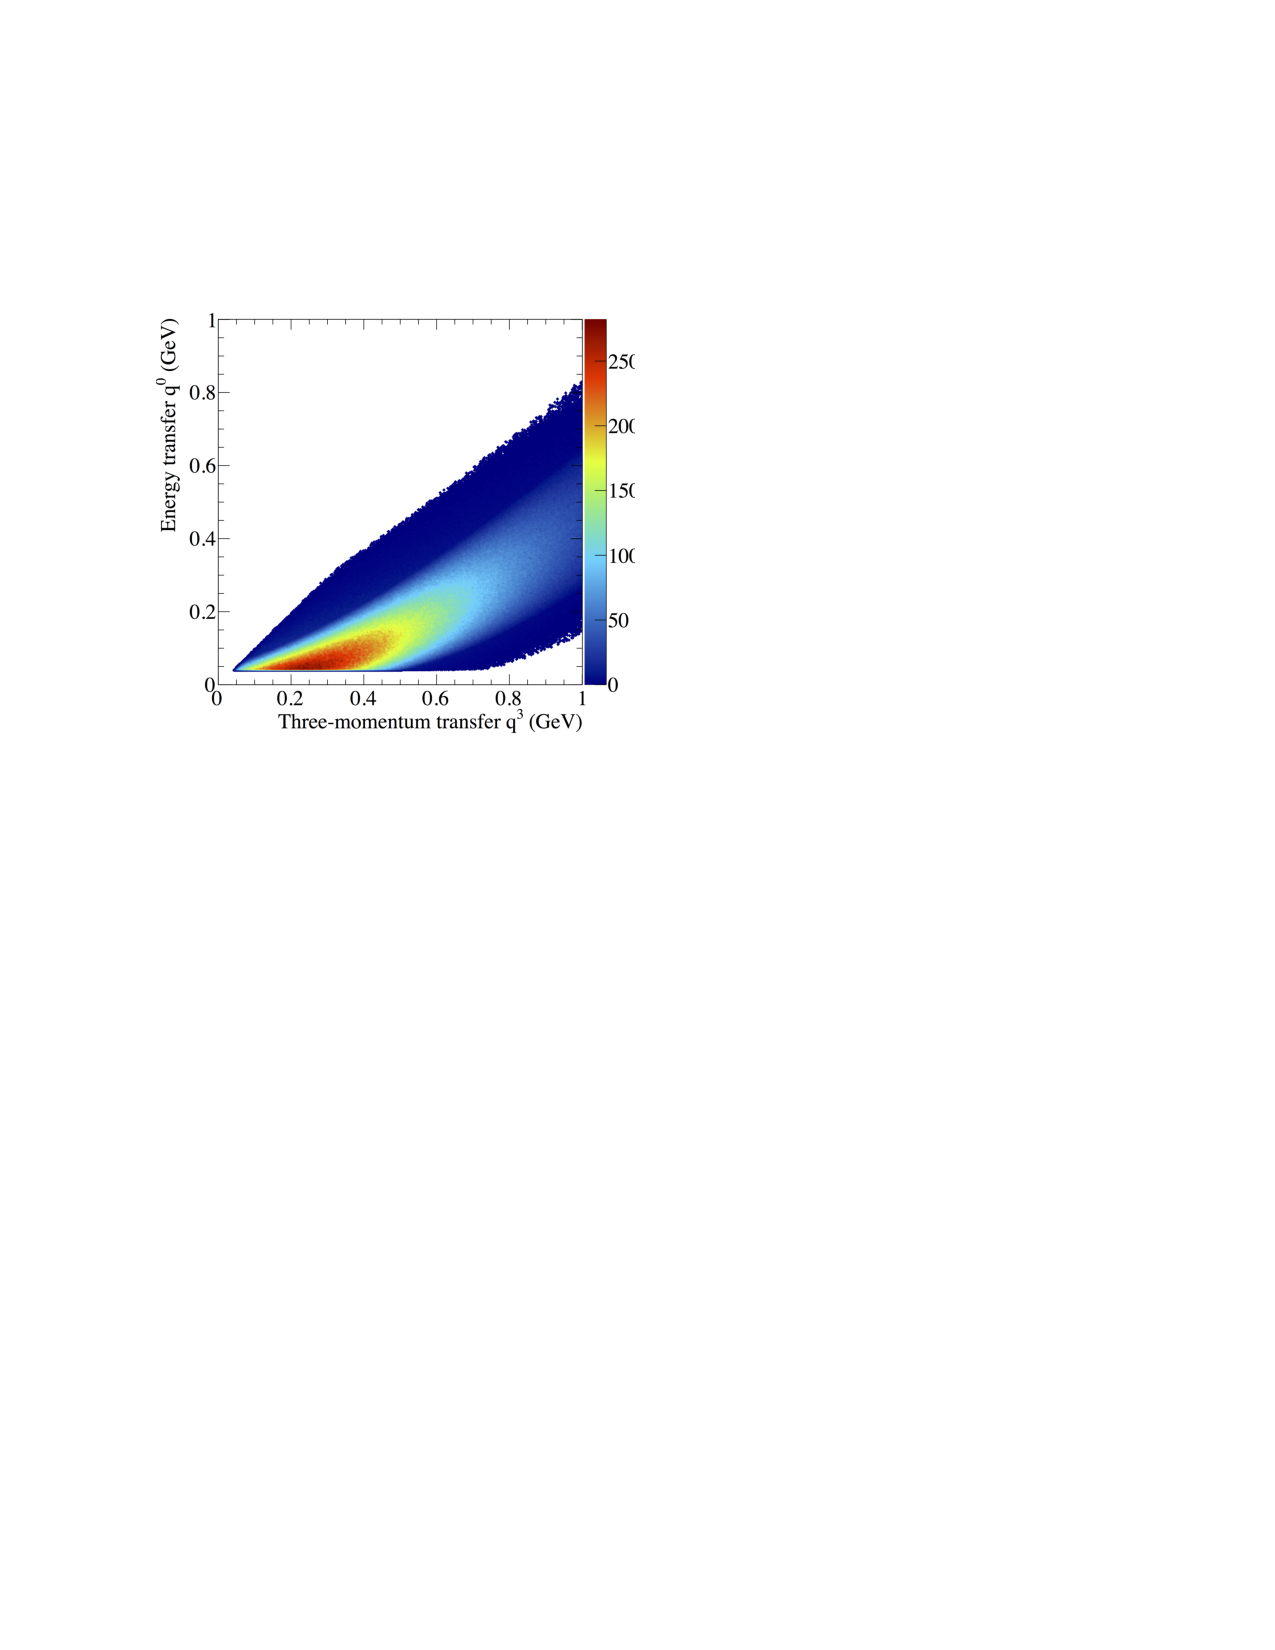
\includegraphics[width=.40\textwidth]{images/QE_MEC_Systematics/qe_default}
   \label{fig:qe_default}} \quad
\subfloat[][Valencia model, kinematics of \acrshort{cc} \acrshort{qe} events.]
   {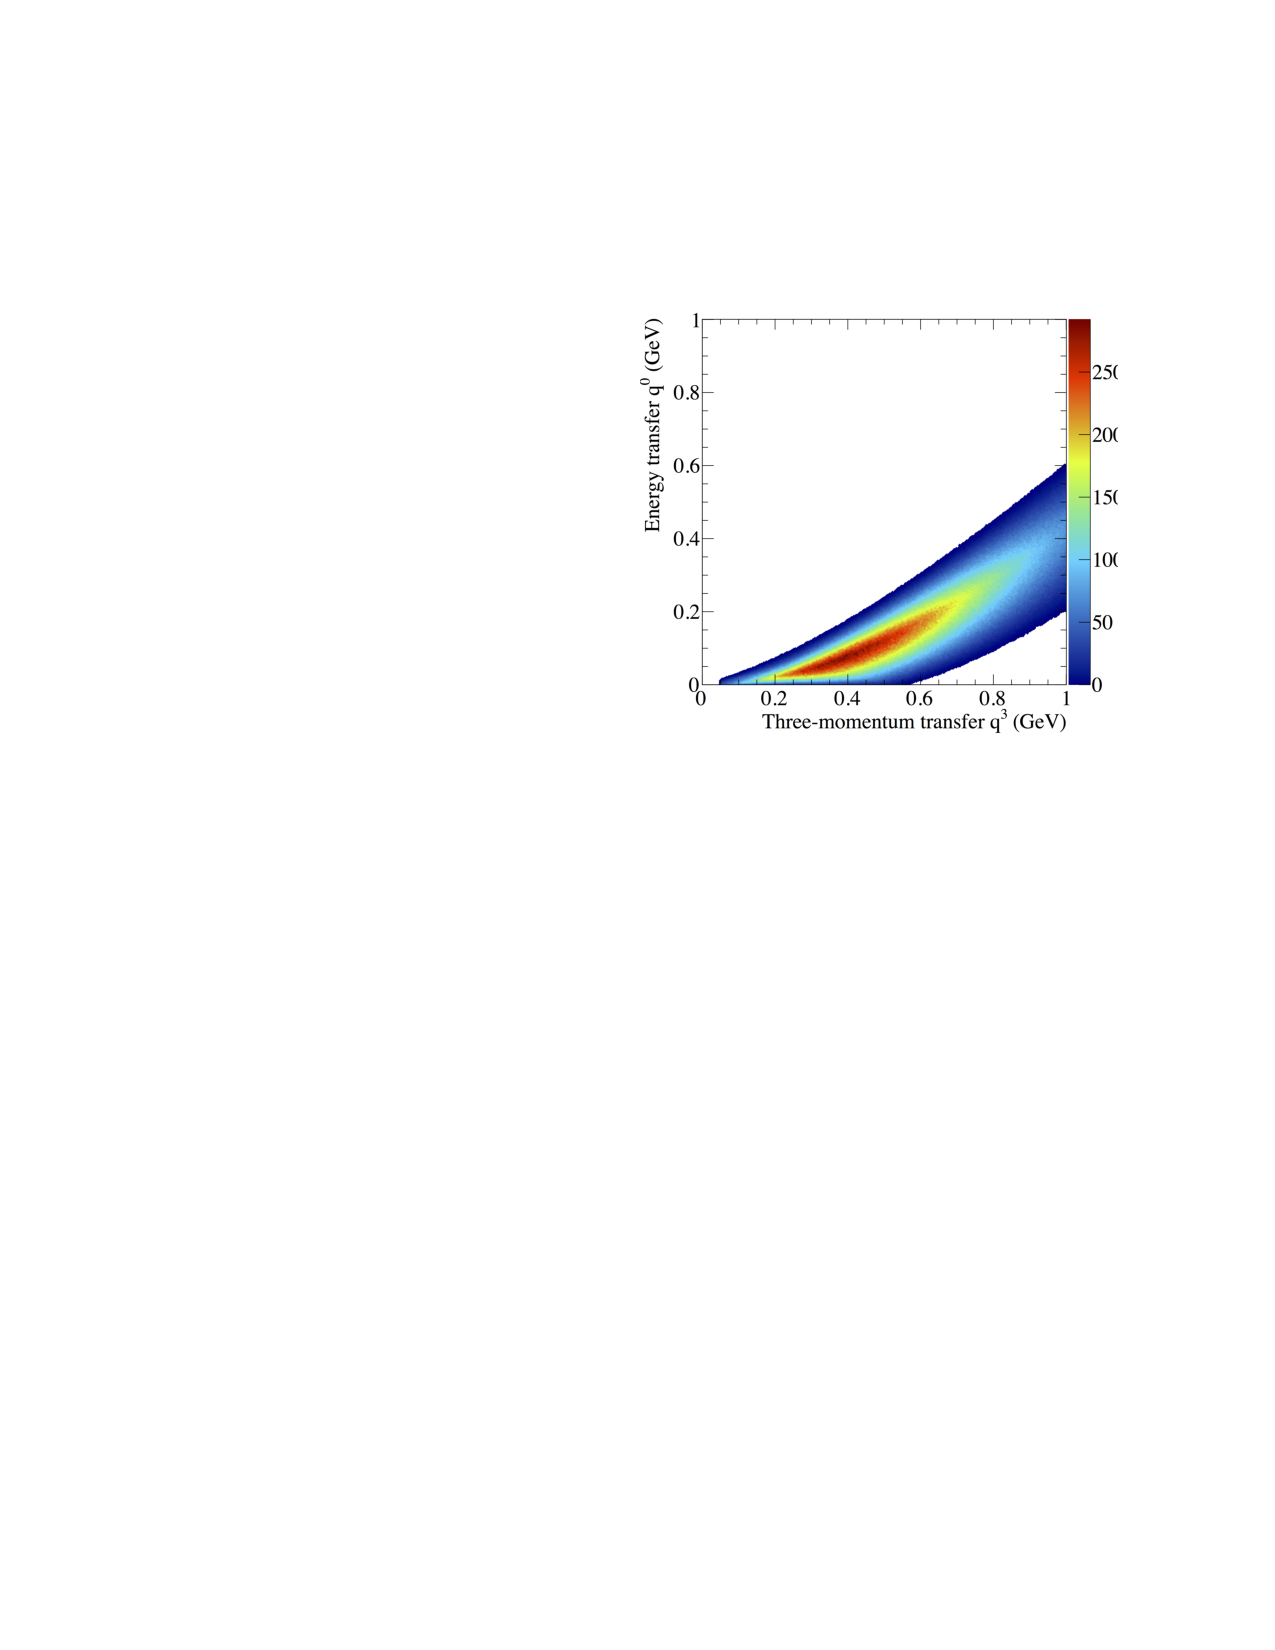
\includegraphics[width=.40\textwidth]{images/QE_MEC_Systematics/qe_valencia}
   \label{fig:qe_valencia}} \\
\subfloat[][Default model, kinematics of \acrshort{cc} \acrshort{mec} events.]
   {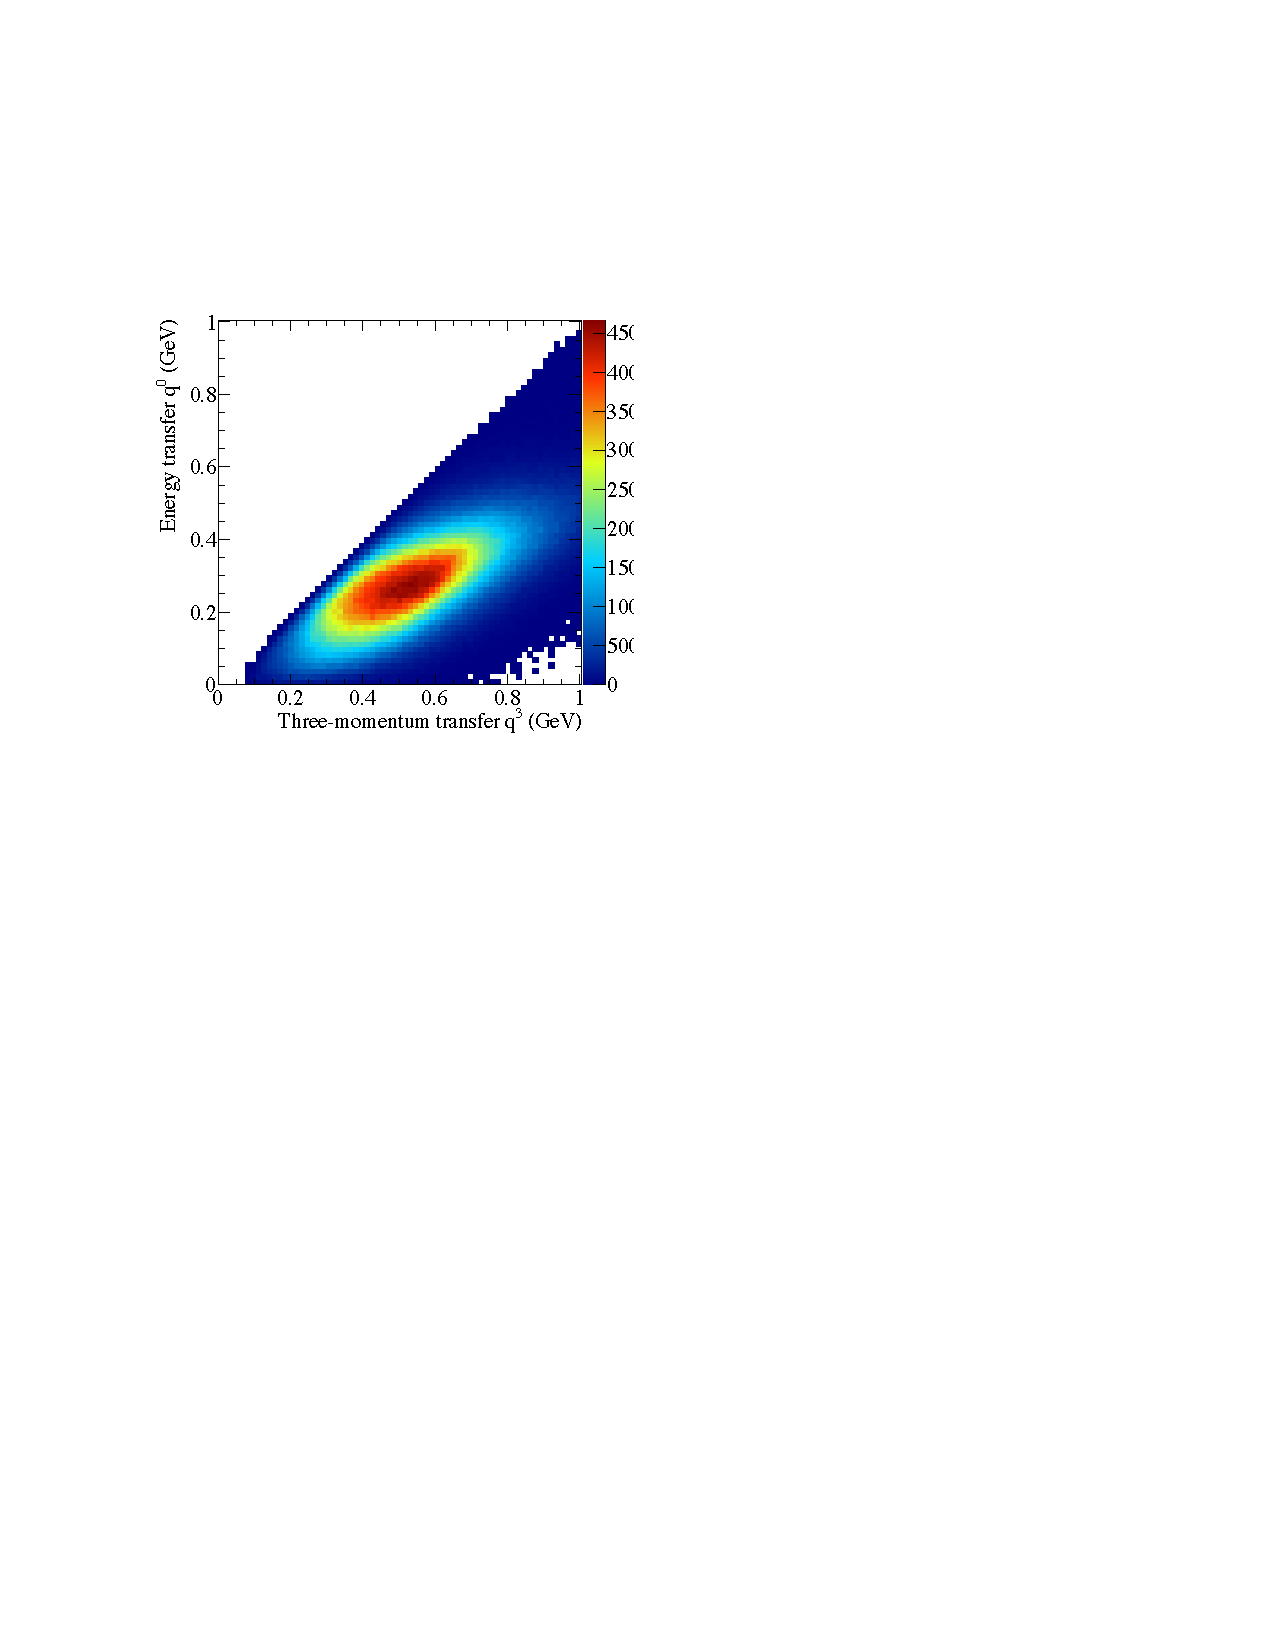
\includegraphics[width=.40\textwidth]{images/QE_MEC_Systematics/mec_default}
   \label{fig:mec_default}} \quad
\subfloat[][Valencia model, kinematics of \acrshort{cc} \acrshort{mec} events.]
   {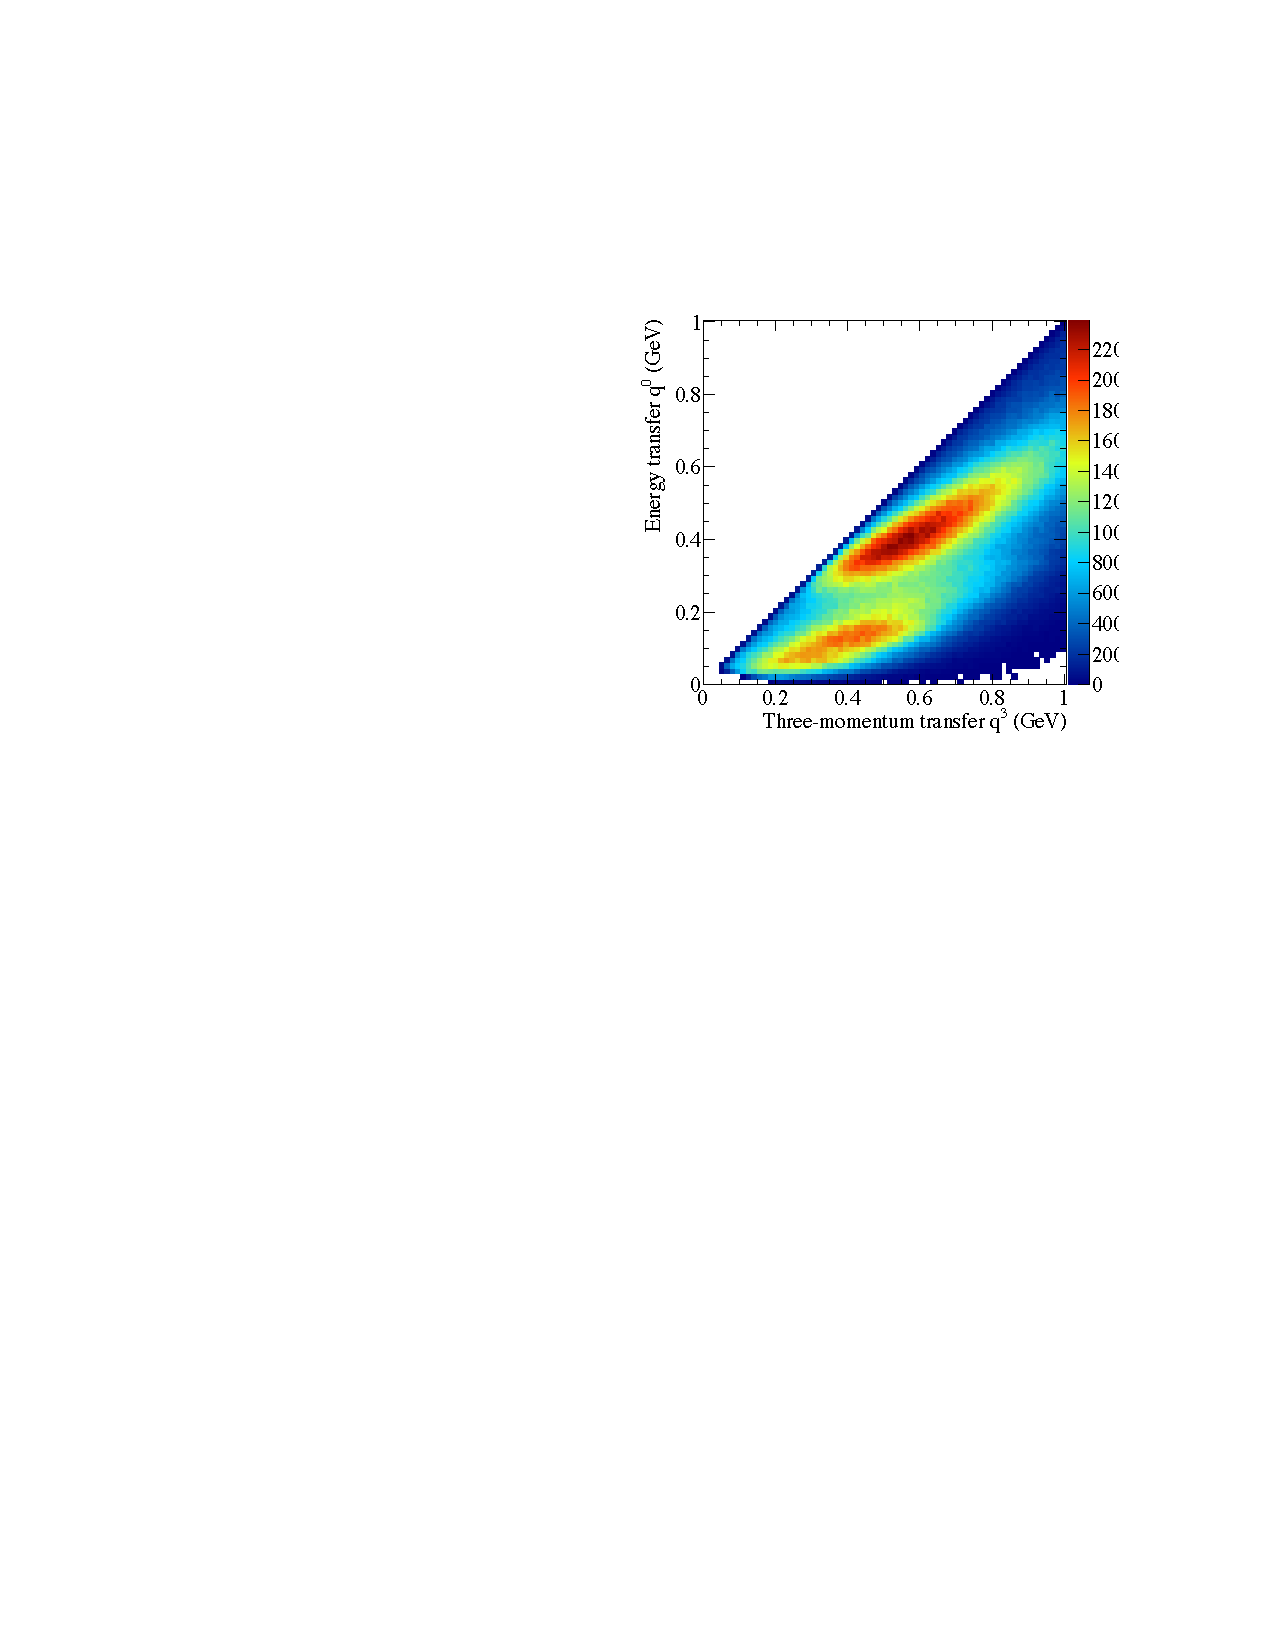
\includegraphics[width=.40\textwidth]{images/QE_MEC_Systematics/mec_valencia}
   \label{fig:mec_valencia}} \\
\caption[\acrshort{cc} \acrshort{qe} and \acrshort{mec} Cross Sections for the Valencia and Default \g Model]{\protect\subref{fig:mastbaum_qe} and~\protect\subref{fig:mastbaum_mec}: \acrshort{cc} \acrshort{qe} and \acrshort{mec} cross sections for the ``Valencia'' and ``Default'' \g models (as extracted from \g
splines), together with the \acrshort{bnb} $\nu_\mu$ flux. \protect\subref{fig:qe_default}, \protect\subref{fig:qe_valencia}, \protect\subref{fig:mec_default}  and \protect\subref{fig:mec_valencia}: kinematics of \acrshort{cc}\acrshort{qe} distributions. Image source: \cite{mastbaum_qe_mec}.}
\label{fig:mastbaum_qe_mec}
%\end{adjustwidth}
\end{figure}


These uncertainties are additional to the default parameter variations built within \g, which are based on fits to historical neutrino scattering data. 
The reweighing is done in the $q^0/q^3$ space, the ratio of area-normalised $q^0/q^3$ distributions is treated as a shape uncertainty, and the ratio of flux-integrated \acrshort{cc}\acrshort{qe} or \acrshort{cc}\acrshort{mec} cross sections as a normalisation uncertainty.

This uncertainty is handled through a \emph{multisim} approach which moves the default \acrshort{mc} toward the ``Valencia'' model by a Gaussian normal distributed random amount, in a set of model variation universes, providing a measure of off-diagonal correlations. In this approach, the upper half of a standard normal is used to draw a normalisation scaling for a given universe, and multiplying this by the ratio between the ``Valencia'' and the ``default'' models for each event. 

Figure~\ref{fig:ccqe_ccmec_multisim} shows the universes distributions and the central value cross sections.
The relative systematic uncertainty on the total cross section, only due to these \acrshort{cc}\acrshort{qe} and \acrshort{cc}\acrshort{mec} uncertainties, amounts to 1.44\%.

\begin{figure}[t]
%\begin{adjustwidth}{-1cm}{-1cm}
\centering
\subfloat[][$d\sigma/dp_\mu$ extracted cross sections.]
   {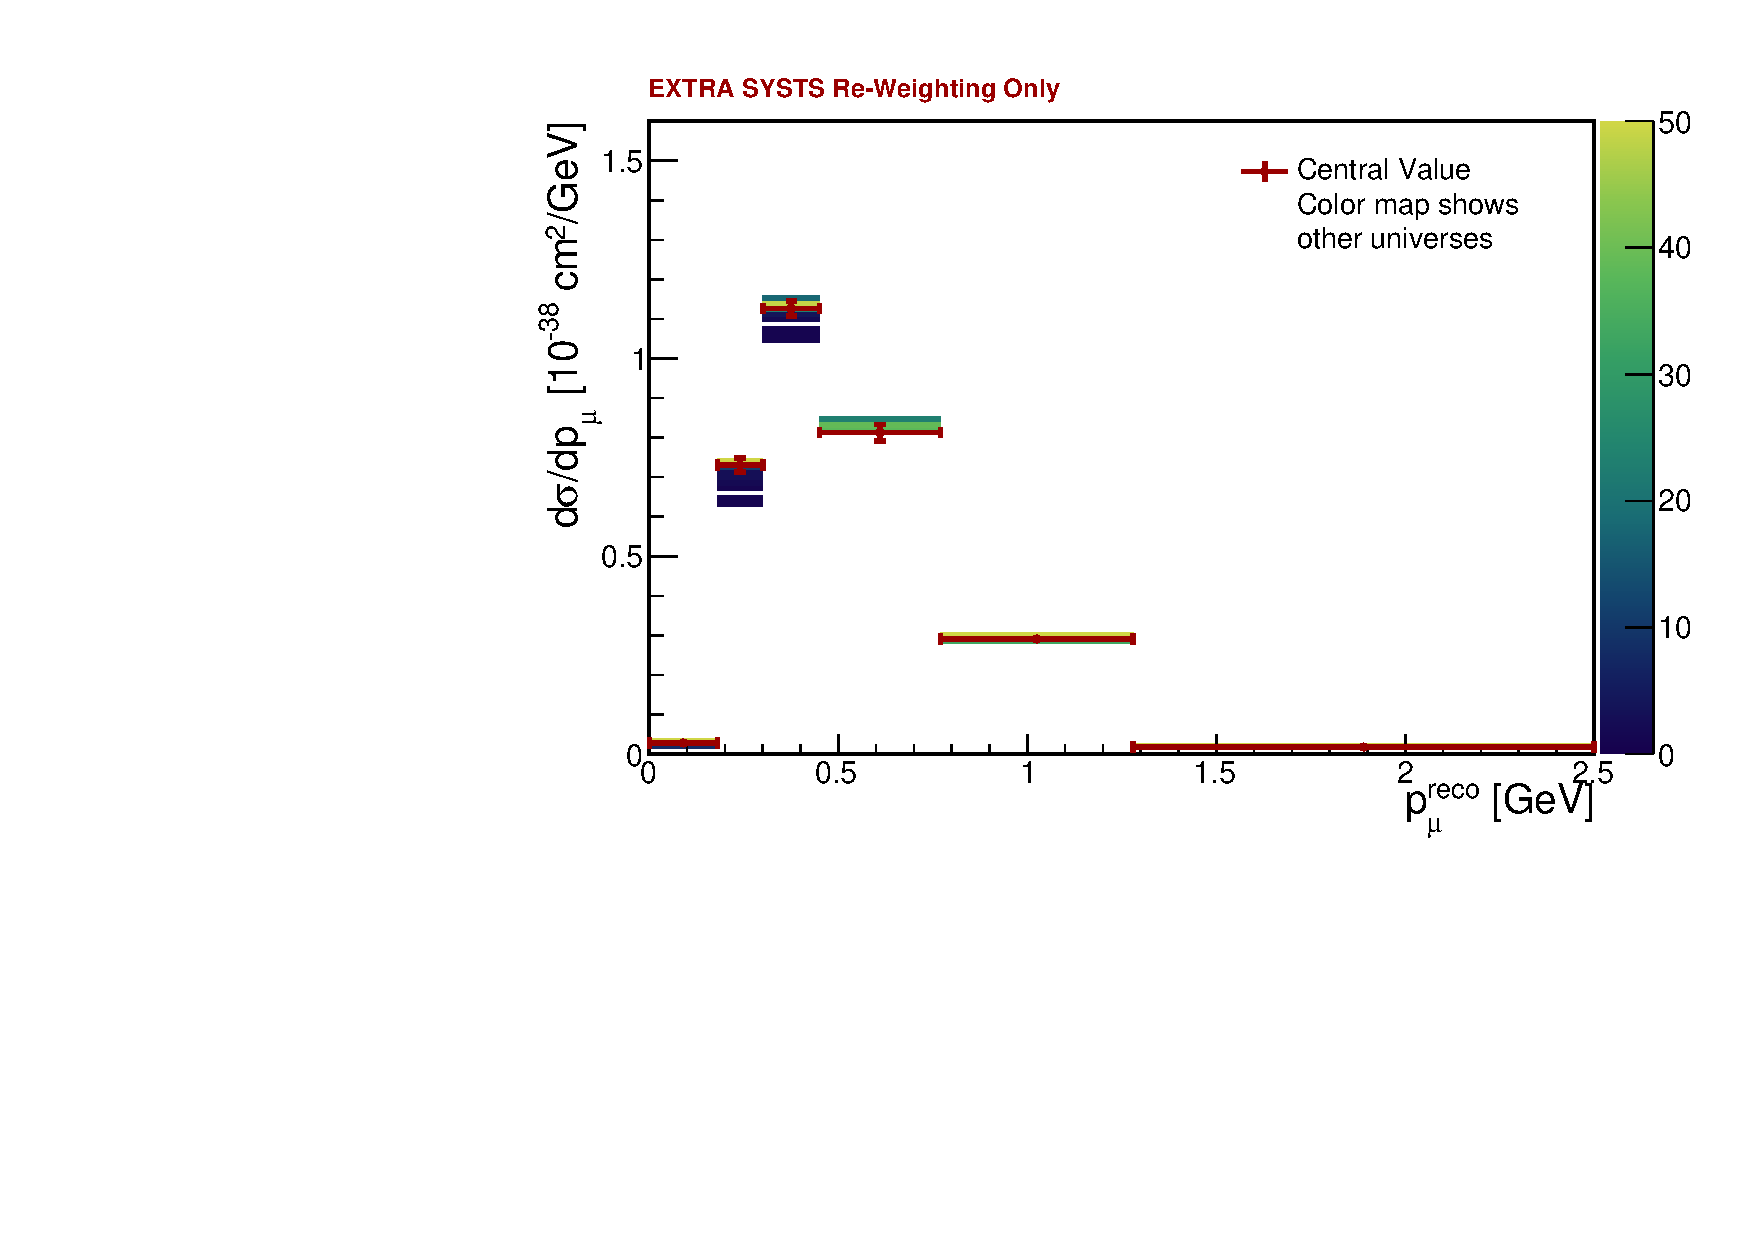
\includegraphics[width=.5\textwidth]{images/ccqe_ccmec_covariance_plots/extra_syst_mumom_xsec_all_fancy}
   \label{fig:ccqe_ccmec_mumom_xsec_all_fancy}}
\subfloat[][$d\sigma/d\cos\theta_\mu$ extracted cross sections.]
   {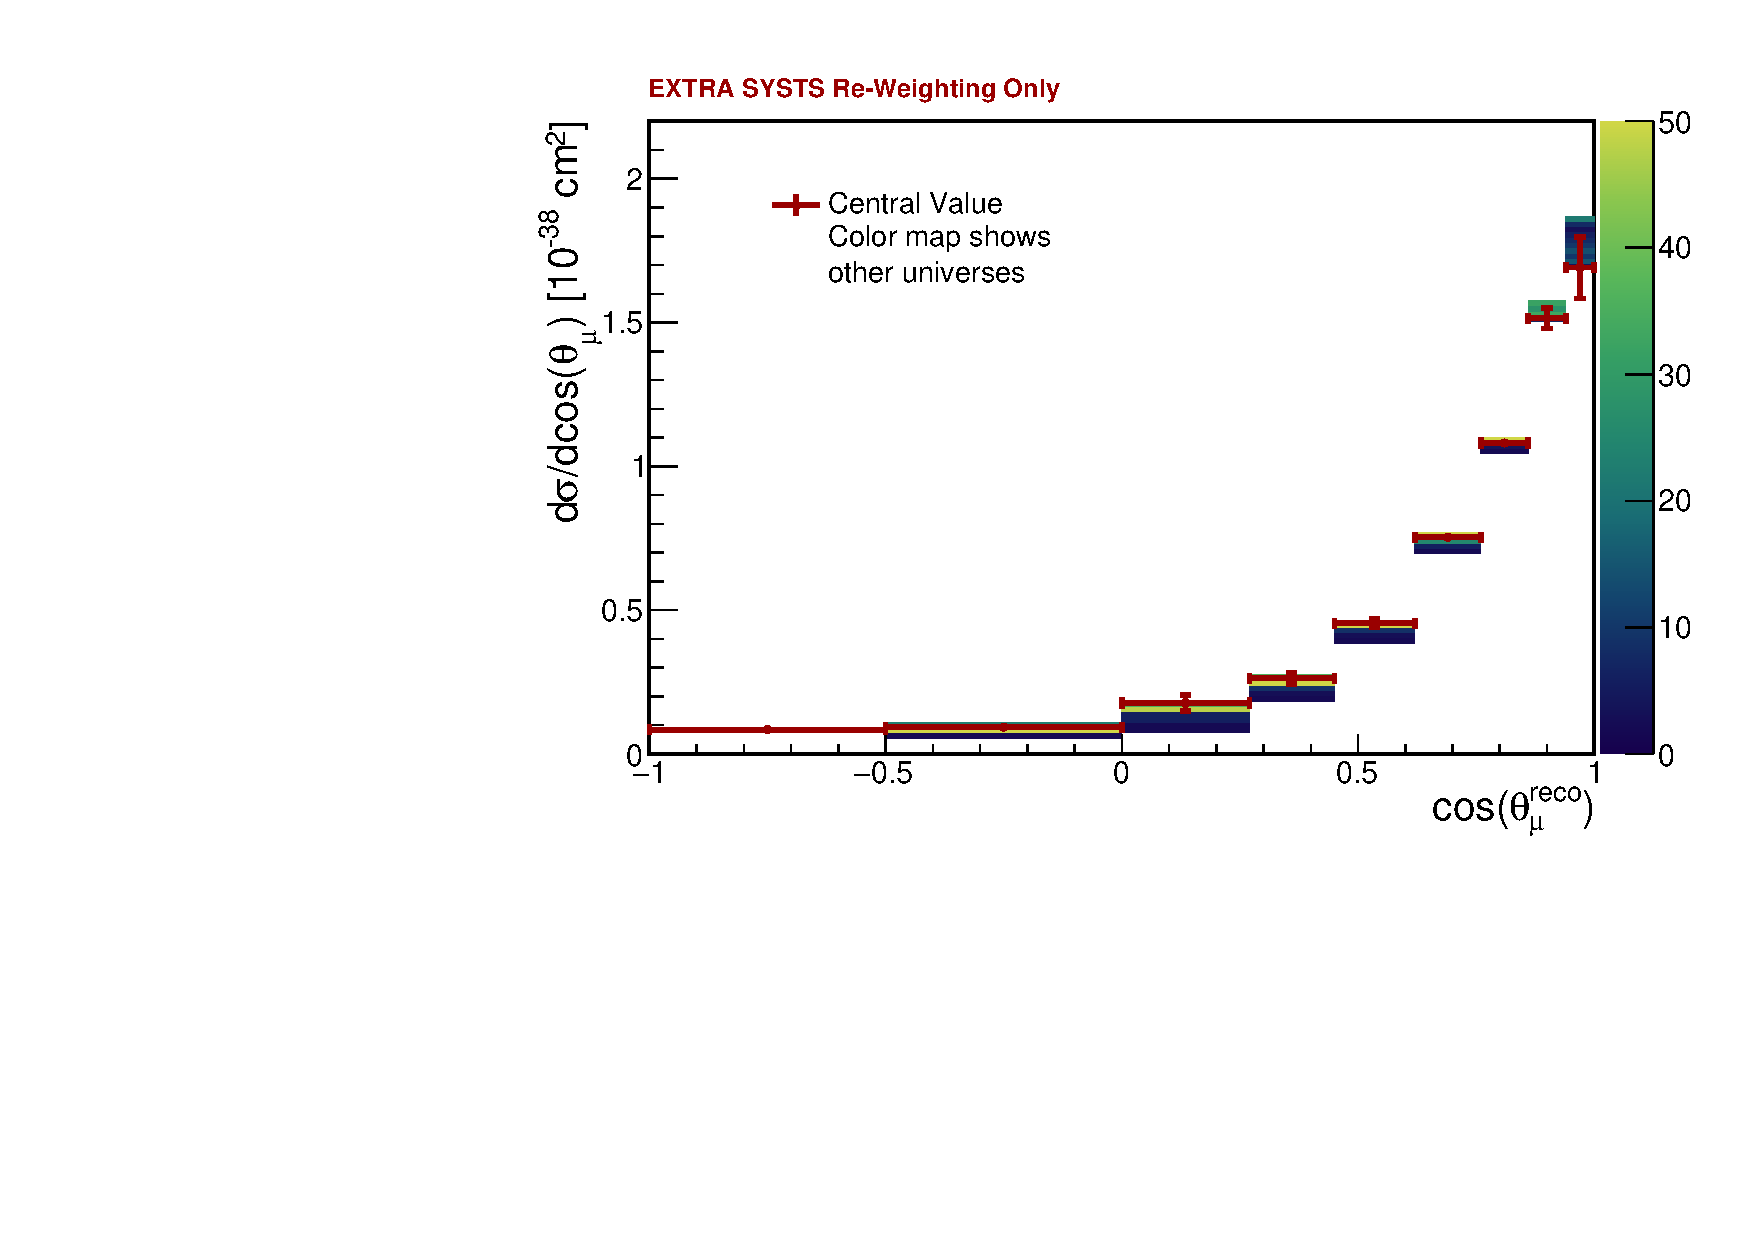
\includegraphics[width=.5\textwidth]{images/ccqe_ccmec_covariance_plots/extra_syst_muangle_xsec_all_fancy}
   \label{fig:ccqe_ccmec_muangle_xsec_all_fancy}}
\caption[\acrshort{cc} \acrshort{qe} and \acrshort{mec} Uncertainties - Universes Distributions]{\emph{\acrshort{cc} \acrshort{qe} and \acrshort{mec} Uncertainties.} Data extracted differential cross sections in muon momentum~\protect\subref{fig:ccqe_ccmec_mumom_xsec_all_fancy} and cosine of the muon angle~\protect\subref{fig:ccqe_ccmec_muangle_xsec_all_fancy} for all simulated universes in the colour map. Only \acrshort{cc}\acrshort{qe} and \acrshort{cc}\acrshort{mec} variations are included in these plots. The red graph shows the data extracted cross section for the nominal \acrshort{mc}. The red vertical bars show the uncertainties derived from the \emph{multisims} according to Equation~\eqref{eq:cov_syst_uni}.}
\label{fig:ccqe_ccmec_multisim}
%\end{adjustwidth}
\end{figure}







\subsection{Hadronic Re-Interaction Systematics}
\label{sec:error_reint}


This section describes the method used to account for uncertainties in the hadron interaction cross-section model that is used in GEANT4. 
Protons, charged pions, and neutrons all lose energy through ionisation but also hadronic scatters with argon nuclei. Hadronic scatters lead to ``hard'' direction changes, or production of new particles.
The interaction length at a given energy is given by:
\begin{equation}
\lambda(E) = \frac{1}{\sigma(E) \cdot \rho},
\end{equation}
where $\sigma(E)$ is the interaction cross section and $\rho$ is the particle number density. For any small piece of pion track, the survival probability (the probability that does not interact) is
\begin{equation}
P_\text{surv}(E, E + \Delta E) = e^{-\Delta L / \lambda(E)},
\end{equation}
where $\Delta L$ is the length of a slice $\Delta L = \Delta E / (dE/dx)$.
Multiplying $P_\text{surv}(E, E + \Delta E)$ for al the pion track segments, the total survival probability at a given initial energy $P_\text{surv}(E_\text{init})$ can be obtained. The interaction probability is then  $P_\text{int}(E_\text{init}) = 1 - P_\text{surv}(E_\text{init})$.
To account for uncertainty in the cross section $\sigma(E)$, such cross section is changed according to its uncertainty and the survival probability is recalculated for a given start momentum, obtaining $P'_\text{surv}$. A conservative estimate to the fractional hadron interaction cross section has been estimated to be 30\%, by looking at data from~\cite{pion_reint_1, pion_reint_2, pion_reint_3}. The weight given to an interacting hadron is:
\begin{equation}
w = \frac{1 - P'_\text{surv}(E_\text{init})}{1 - P_\text{surv}(E_\text{init})},
\end{equation}
while the weight given to a non-interacting hadron is:
\begin{equation}
w = \frac{P'_\text{surv}(E_\text{init})}{P_\text{surv}(E_\text{init})}.
\end{equation}
This reweighting is performed on a per-event basis and the results is shown in Figure~\ref{fig:reinteraction_multisim}.
The relative systematic uncertainty on the total cross section, only due to particle re-interaction uncertainties, amounts to 0.612\%.


\begin{figure}[t]
%\begin{adjustwidth}{-1cm}{-1cm}
\centering
\subfloat[][$d\sigma/dp_\mu$ extracted cross sections.]
   {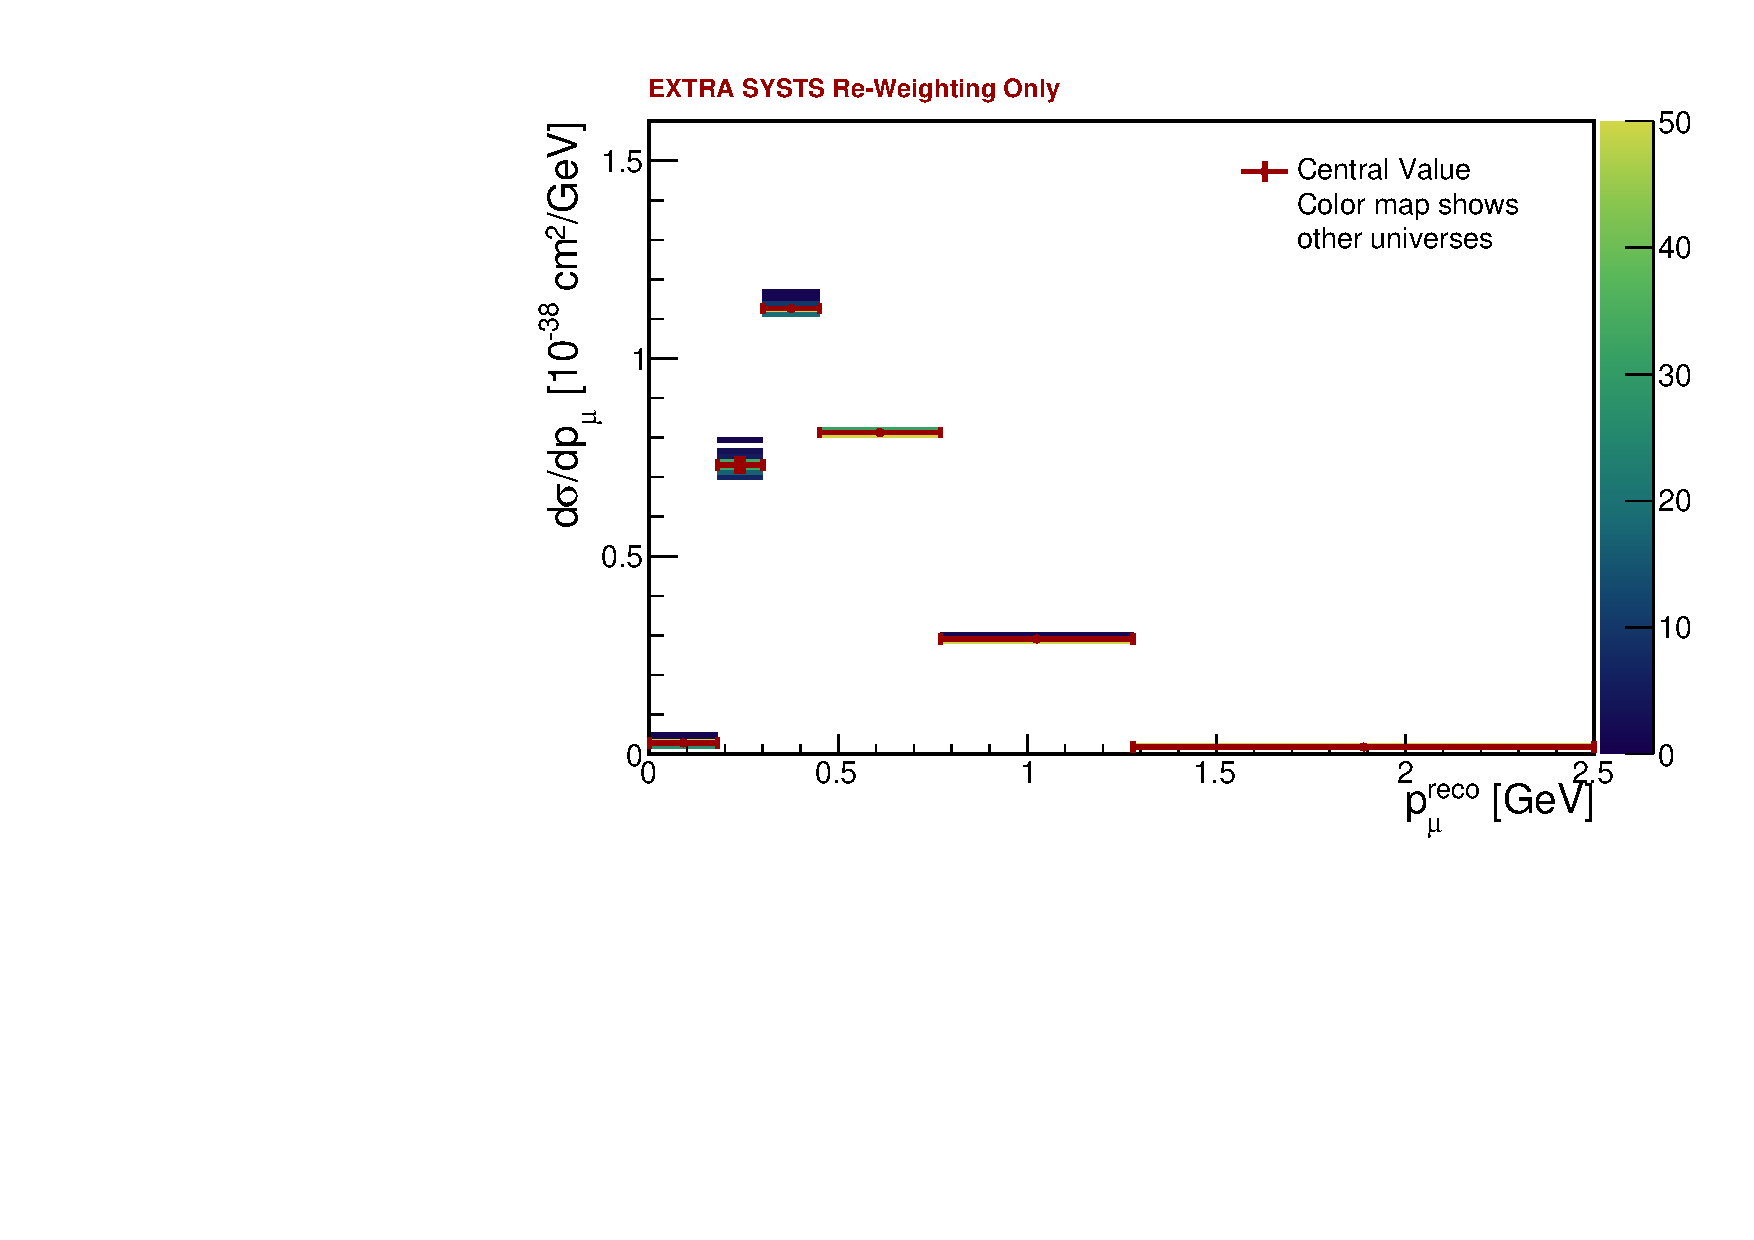
\includegraphics[width=.5\textwidth]{images/reinteraction_covariance_plots/extra_syst_mumom_xsec_all_fancy}
   \label{fig:reinteraction_multisim_mumom_xsec_all_fancy}}
\subfloat[][$d\sigma/d\cos\theta_\mu$ extracted cross sections.]
   {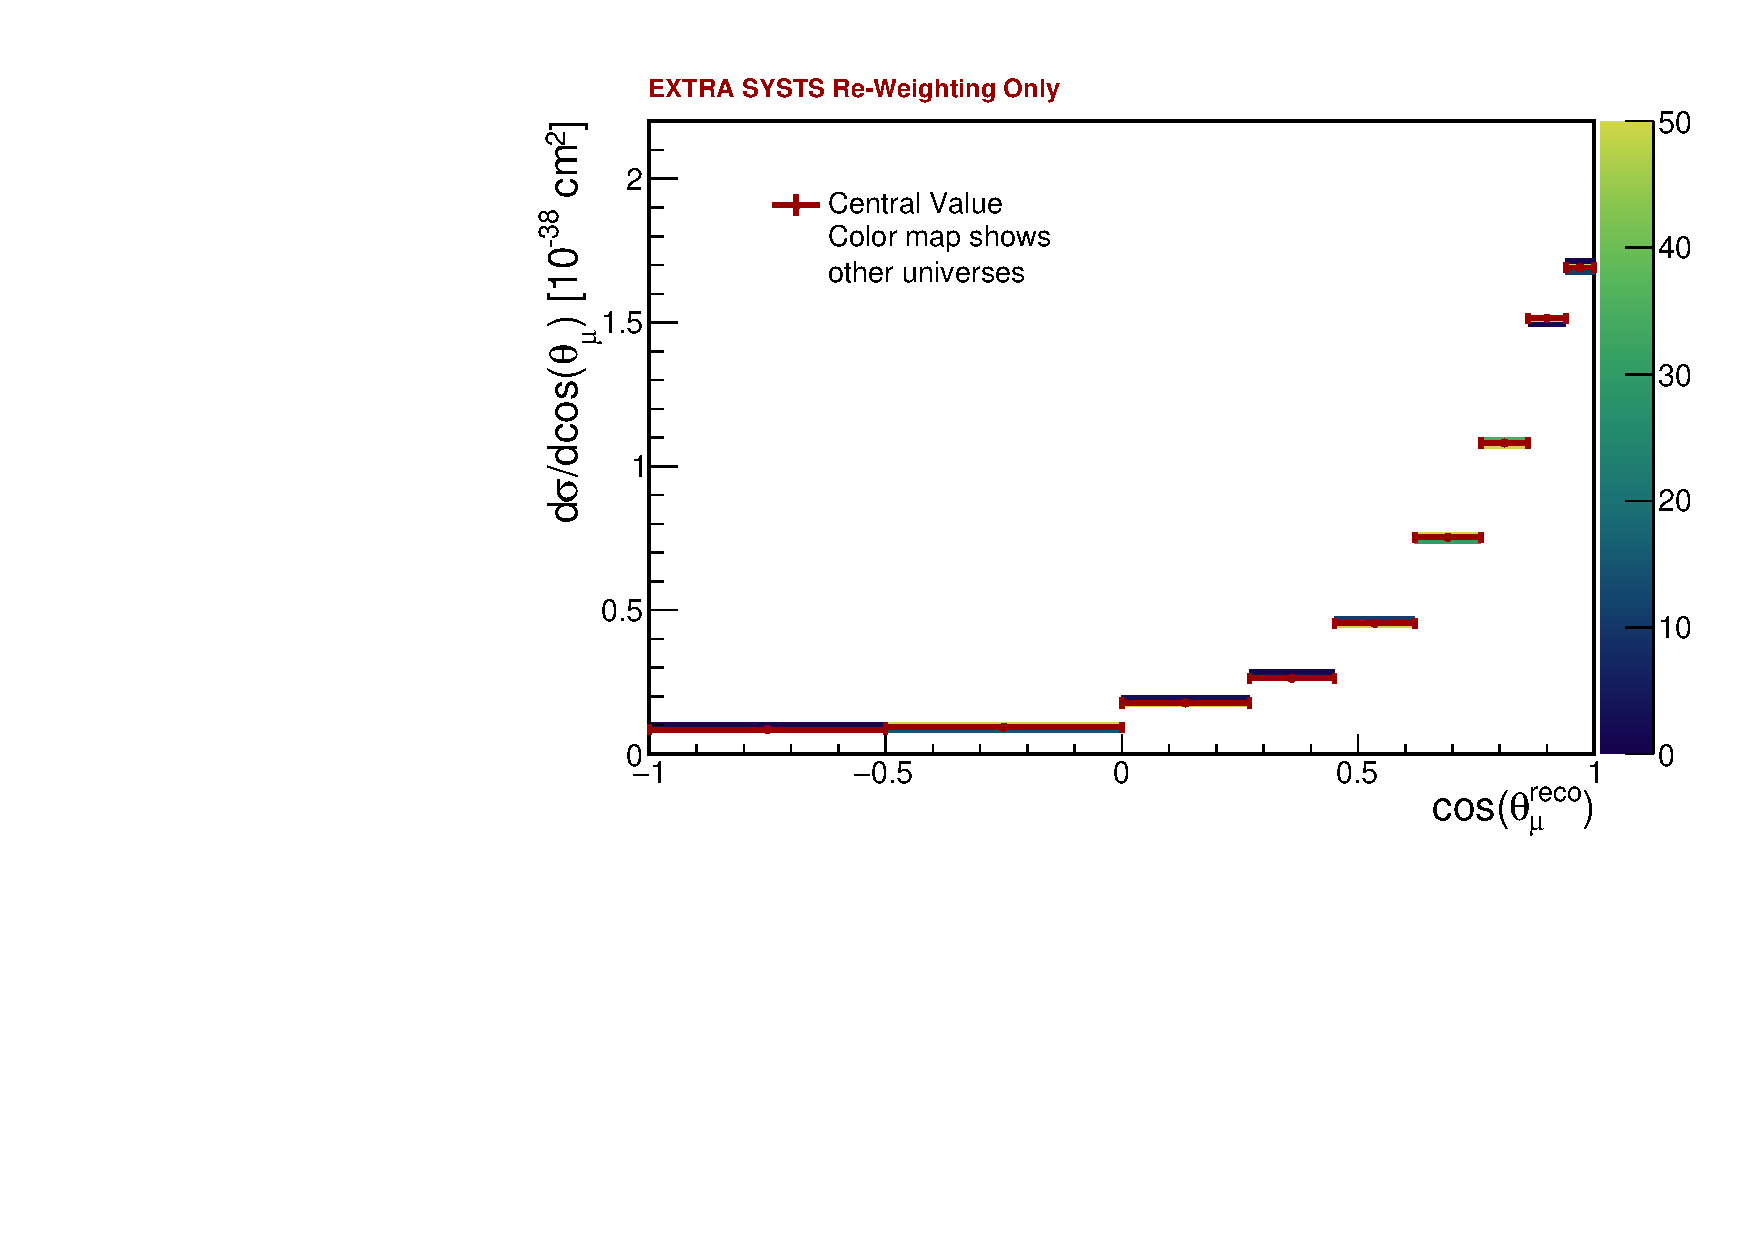
\includegraphics[width=.5\textwidth]{images/reinteraction_covariance_plots/extra_syst_muangle_xsec_all_fancy}
   \label{fig:reinteraction_multisim_muangle_xsec_all_fancy}} 
\caption[Particle Re-Interaction Uncertainties - Universes Distributions]{\emph{Particle Re-Interaction Uncertainties.} 
Data extracted differential cross sections in muon momentum~\protect\subref{fig:reinteraction_multisim_mumom_xsec_all_fancy} and cosine of the muon angle~\protect\subref{fig:reinteraction_multisim_muangle_xsec_all_fancy} for all simulated universes in the colour map. Only particle reinteraction variations are included in these plots. The red graph shows the data extracted cross section for the nominal \acrshort{mc}. The red vertical bars show the uncertainties derived from the \emph{multisims} according to Equation~\eqref{eq:cov_syst_uni}.}
\label{fig:reinteraction_multisim}
%\end{adjustwidth}
\end{figure}




\clearpage
%**********************************************************
\section{Beam Flux Uncertainties}
\label{sec:error_flux}

This section describes the implementation of the beam flux uncertainties, which are divided into two main categories: 
\begin{itemize}
\item uncertainties related to secondary hadron particles ($\pi^+$, $\pi^-$, $K^0$, $K^+$, $K^-$) due to the collision of protons with the beryllium target;
\item ``non-hadron'' uncertainties, arising from uncertainties in the estimation of the current running in the horn conductor, as well as the estimation of the depth of the conductor traversed by such current (``skin effect''), and the estimation of  the pion and nucleon cross sections (total, inelastic, and \acrshort{qe}) on aluminium and beryllium.
\end{itemize} 
In total, there are six uncertainties due to flux modelling: five on hadron production and one on non-hadron production. 
1000 \emph{multisims} are generated where the flux parameters are varied. The non-hadron uncertainties are estimated by varying the effect by plus or minus one standard deviation. In the case of the ``skin effect'', the model is switched on and off to create a second universe. The two universes are used to generate weights to assess the overall systematic uncertainties by assuming they follow a Gaussian distribution around the central value. The covariance matrix is calculated according to Equation~\eqref{eq:cov_syst_uni}.

The re-weighting of the hadron production cross sections is described in \cite{miniboone_flux, flux_note}. This section focuses on the evaluation of the $\pi^+$ uncertainties, as they have the largest impact on the final cross-section uncertainty. The beam simulation used at MicroBooNE uses as a central value a Sanford-Wang~\cite{miniboone_flux} parameterisation based on fits to data provided by the HARP experiment \cite{schmitz}. HARP provided double-differential charged pion production cross sections at the Booster energies, with a full covariance matrix. The systematic uncertainties are assessed performing a splined fit to the HARP cross-section data. Figure \ref{fig:harp_fit} shows the HARP data, the spline fits, and the central value fit. A visible bias is introduced such that the average of the universes drawn from the splining is offset from the nominal central value. 
\begin{figure}[]
\centering
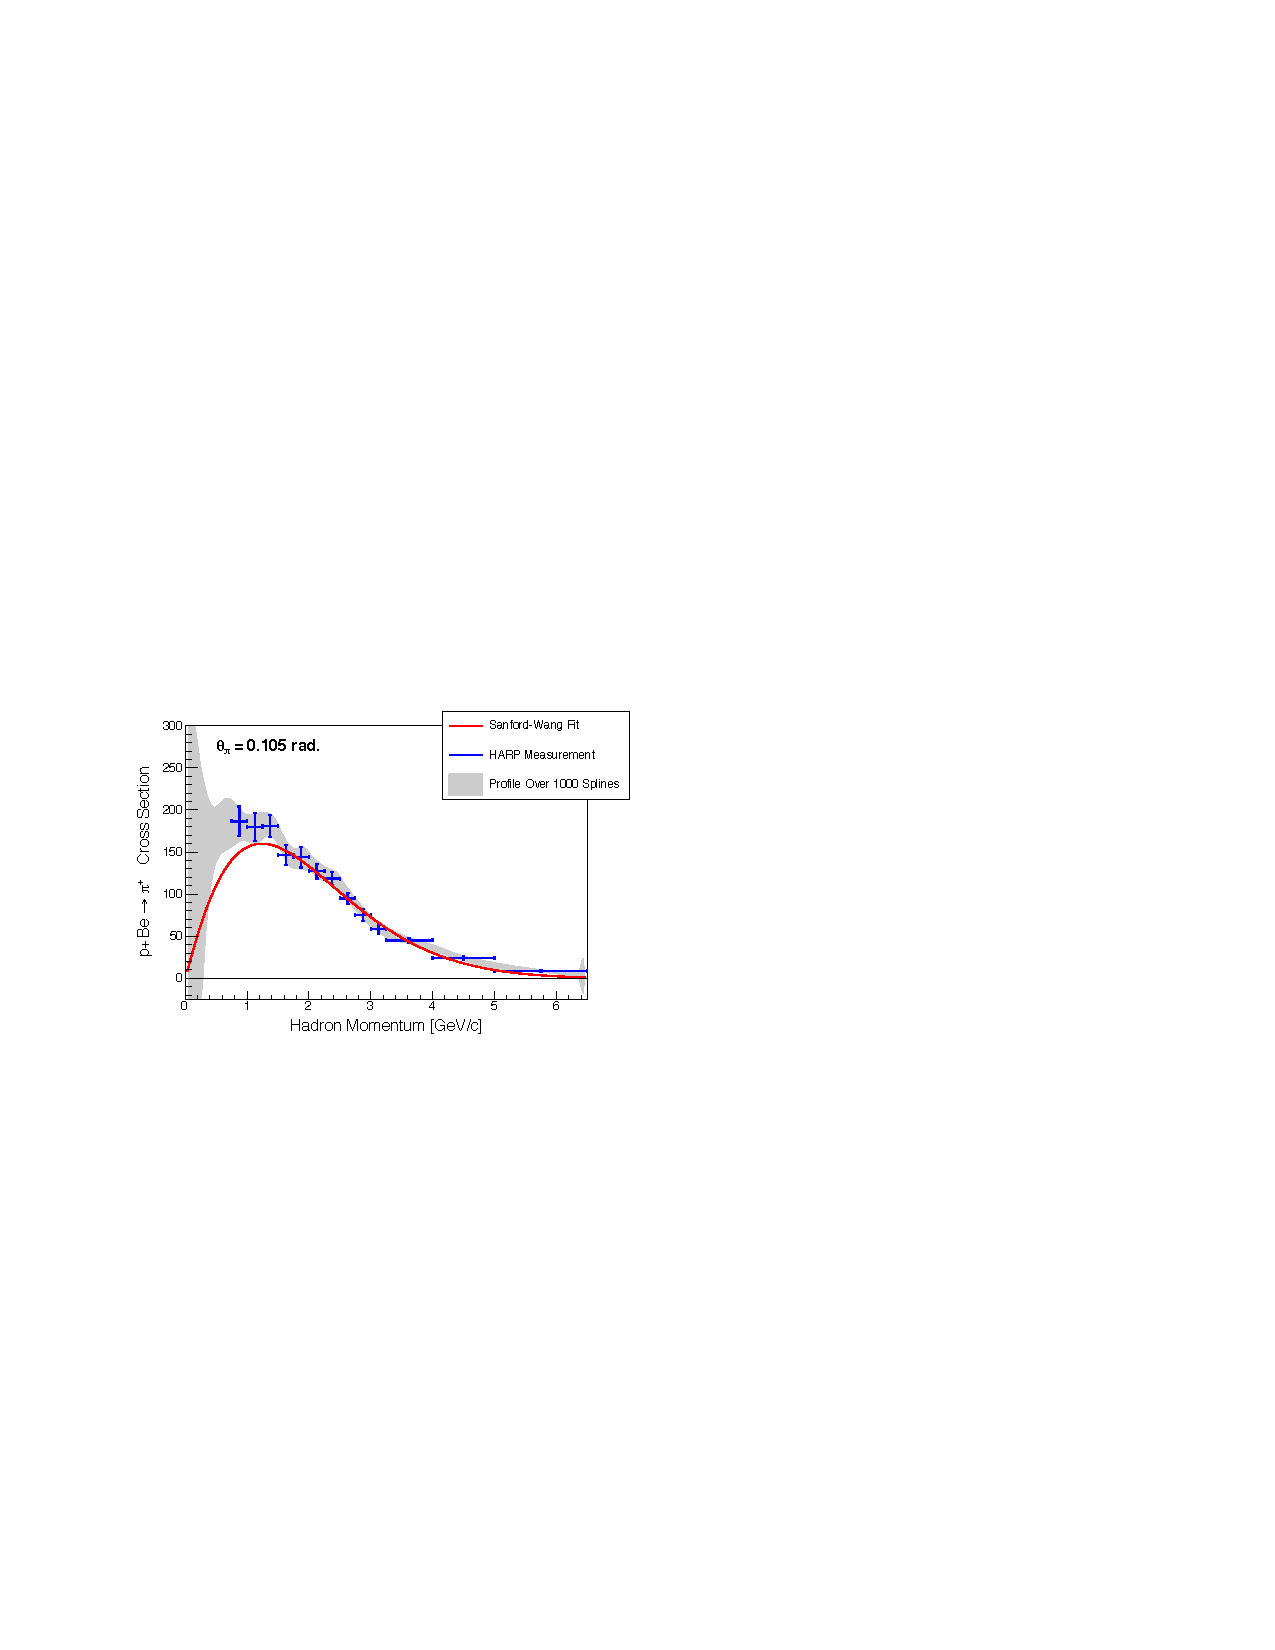
\includegraphics[width=.70\textwidth]{images/harp_fit}
\caption[HARP Pion Production Cross Section Measurements]{HARP pion production cross section measurements as a function of outgoing hadron momentum at a fixed hadron angle ($\theta_\pi$ = 0.105 rad.). The plot includes the measurements, in blue, the Sanford-Wang parameterisation, in red, and the profile of 1000 spline fits to correlated variations in the HARP measured cross sections, in grey. Image source: \cite{flux_technote}.}
\label{fig:harp_fit}
\end{figure}
This creates a bias between the cross-section central value and the average of the cross section among all the universes. Figure~\ref{fig:flux_multisim_onebin}, illustrating the total cross section for all the universes, and the nominal cross section, clearly shows the bias described above, where almost all the universes predict a cross section smaller than the nominal central value.
As already discussed in the introduction to this chapter, in this case Equation~\eqref{eq:cov_syst_uni} is still used to evaluate the covariance matrix, as this includes the proper covariance matrix $V$ and the bias $B$ as shown in Equation~\eqref{eq:cov_matrix_bias}. Including the bias allows having a conservative estimate for the flux systematic uncertainties. The red vertical bars in this plot are the cross-section systematic uncertainties derived from these universes.

The relative uncertainties on the total cross section for all the flux systematic categories are shown in Table~\ref{tab:flux_parameters}. The overall relative flux systematic uncertainty amounts to $12.16\%$, where the main contributions arise from the $\pi^+$ production cross section and the non-hadron systematics. 




%+++++++++TABLE+++++++++
\begin{table}[p]
%\begin{adjustwidth}{-3cm}{-3cm}
\caption[Beam Flux Modelling Systematic Uncertainties]{Flux systematics parameters and their contribution to the relative cross-section uncertainty.}
\label{tab:flux_parameters}
\centering
\begin{tabular}{c c}
\toprule
Parameter                                                        &  Total Cross Section  \\
                                                                 &  Relative Uncertainty \\
\midrule
Non-Hadron                        &  5.46\%   \\
$K^-$ production cross section     &  0.52\%    \\
$K^+$ production cross section    &  0.54\%    \\
$K^0$ production cross section    &  0.57\%    \\
$\pi^-$ production cross section   &  0.75\%    \\
$\pi^+$ production cross section   &  9.59\%    \\
\midrule
Combined uncertainty                                           &  12.16\%    \\
\bottomrule
\end{tabular}
%\end{adjustwidth}
\end{table}
%++++++++++++++++++++++++

\begin{figure}[]
\centering
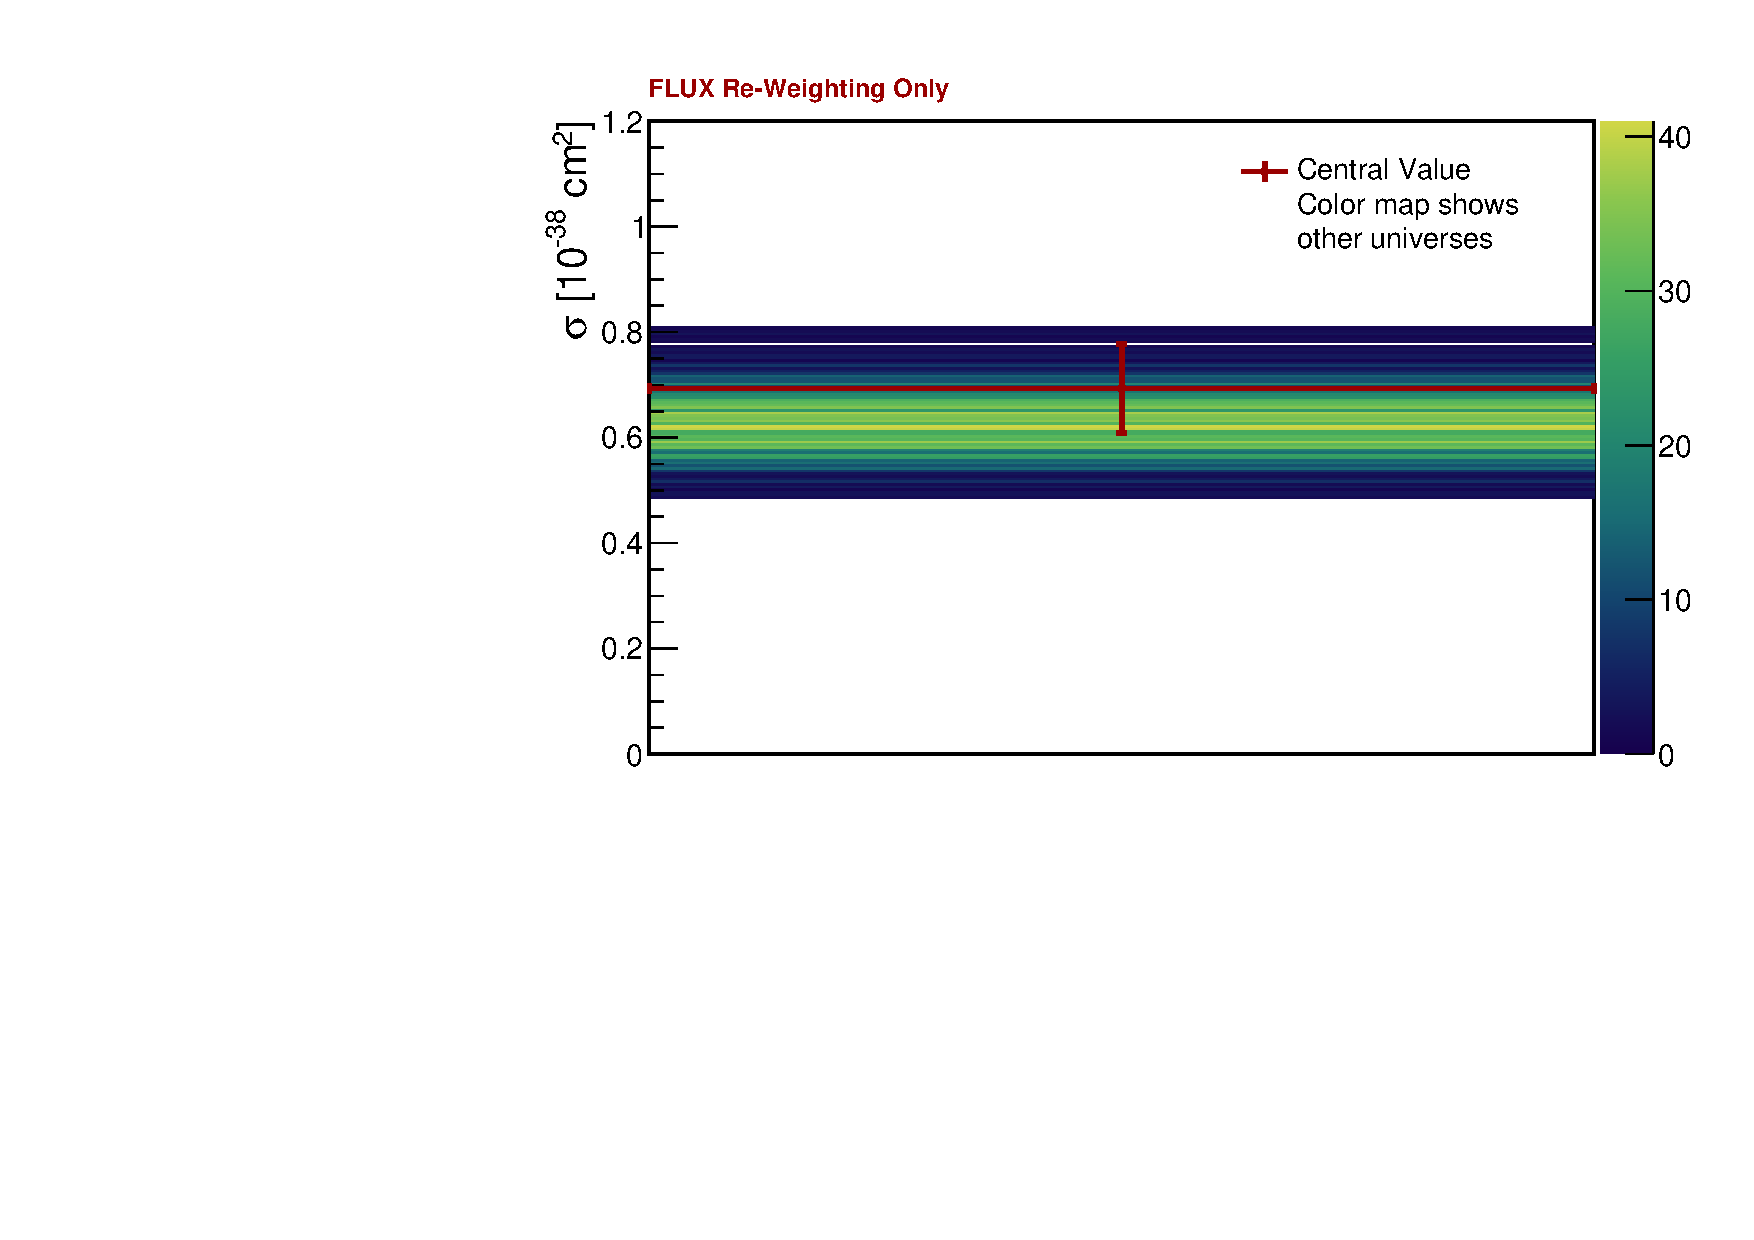
\includegraphics[width=.70\textwidth]{images/flux_covariance_plots/flux_multisim_onebin_xsec_all_fancy}
\caption[Beam Flux Uncertainties - Total Cross Section - Universes Distributions]{\emph{Beam Flux Uncertainties.} Total cross section extracted from data for all the simulated universes in the colour map. The red graph shows the total data extracted cross section for the nominal \acrshort{mc}. The red vertical bars show the flux systematic uncertainty derived from the \emph{multisims} according to Equation~\eqref{eq:cov_syst_uni}. The relative systematic uncertainty on the total cross section is 12.16\%.}
\label{fig:flux_multisim_onebin}
\end{figure}

An additional uncertainty is due to the \acrshort{pot} counting. The primary proton beam is monitored using two toroids measuring its intensity (protons-per-pulse). According to the MiniBooNE flux paper \cite{miniboone_flux}, the proton flux measured in the two toroids agree within 2\% . This is included as an additional uncertainty on the normalisation of the cross section, added in quadrature to all the elements of the final total covariance matrix.


\begin{figure}[t]
%\begin{adjustwidth}{-1cm}{-1cm}
\centering
\subfloat[][$d\sigma/dp_\mu$ extracted cross sections.]
   {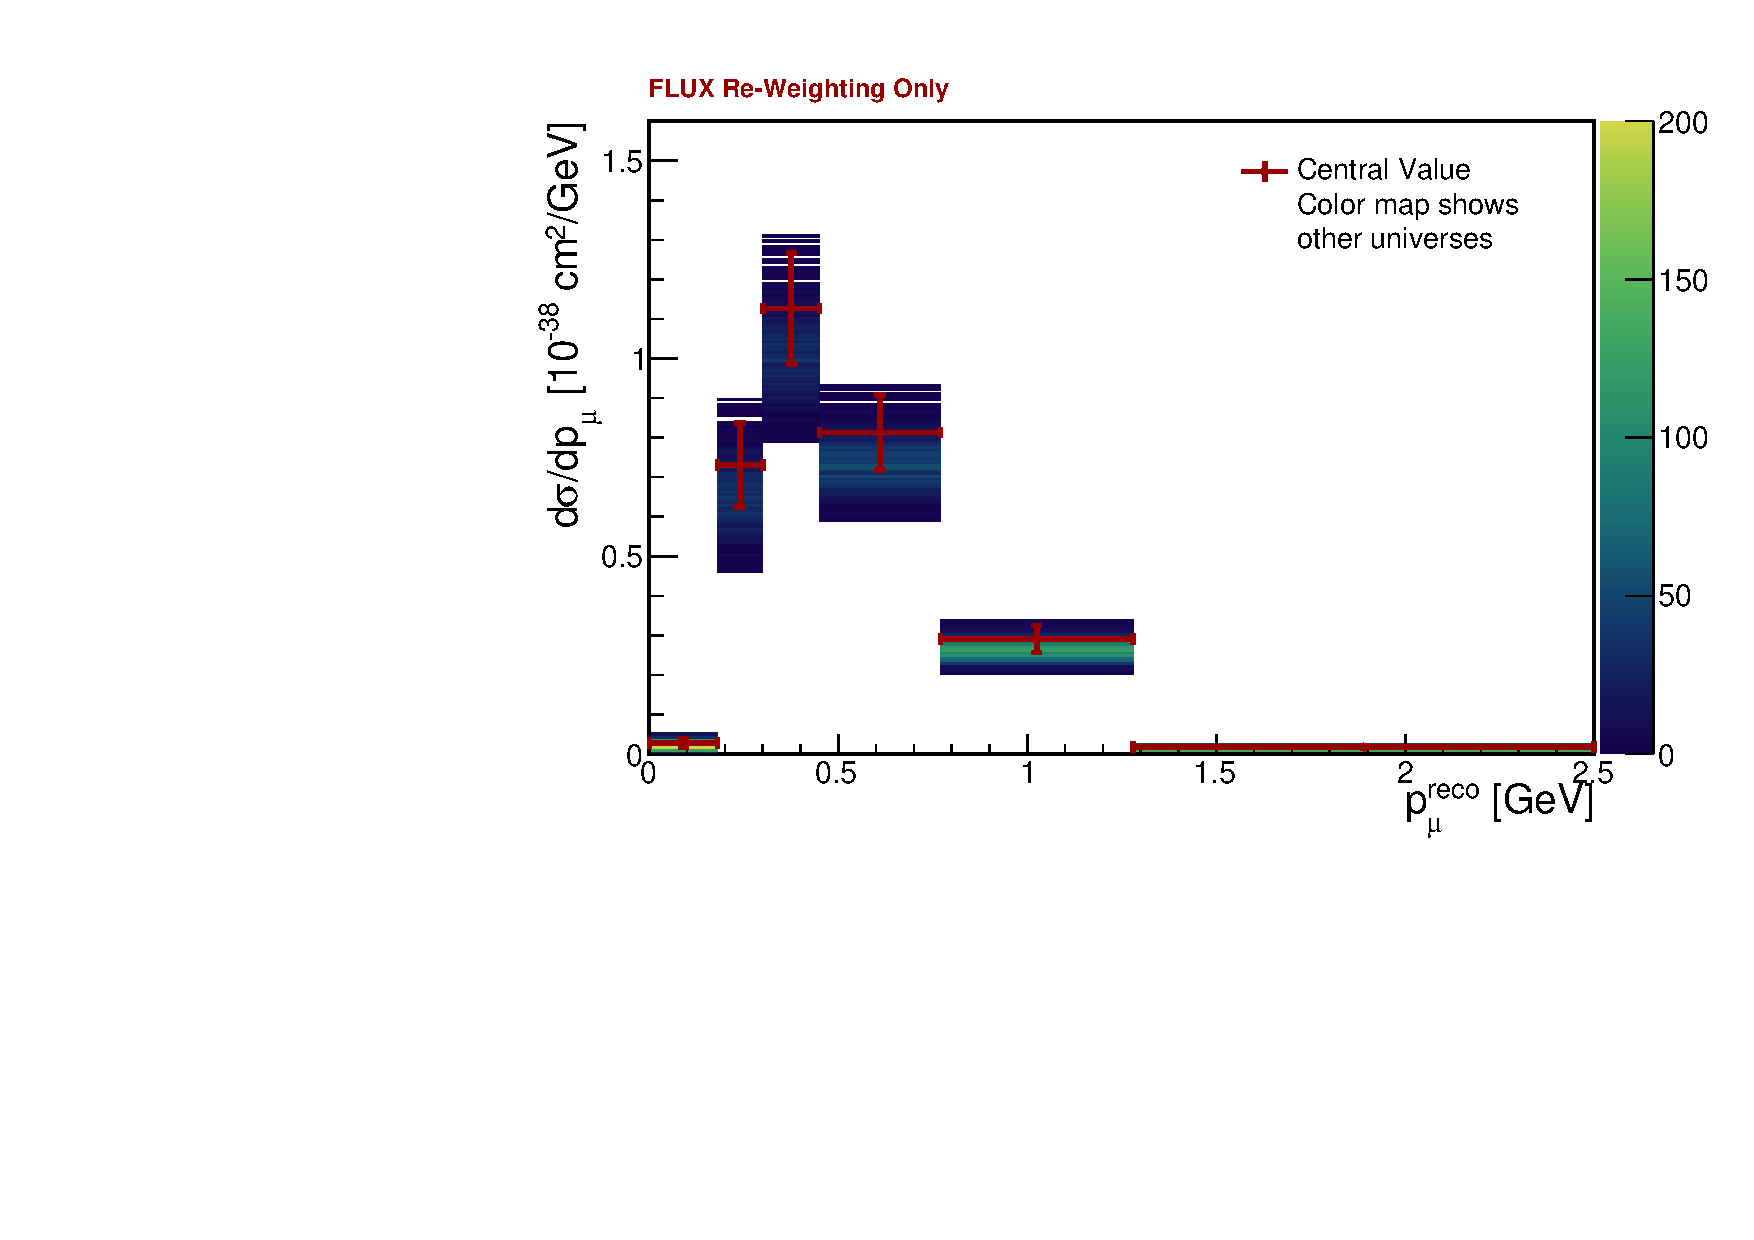
\includegraphics[width=.5\textwidth]{images/flux_covariance_plots/flux_multisim_mumom_xsec_all_fancy}
   \label{fig:flux_multisim_mumom_xsec_all_fancy}}
\subfloat[][$d\sigma/d\cos\theta_\mu$ extracted cross sections.]
   {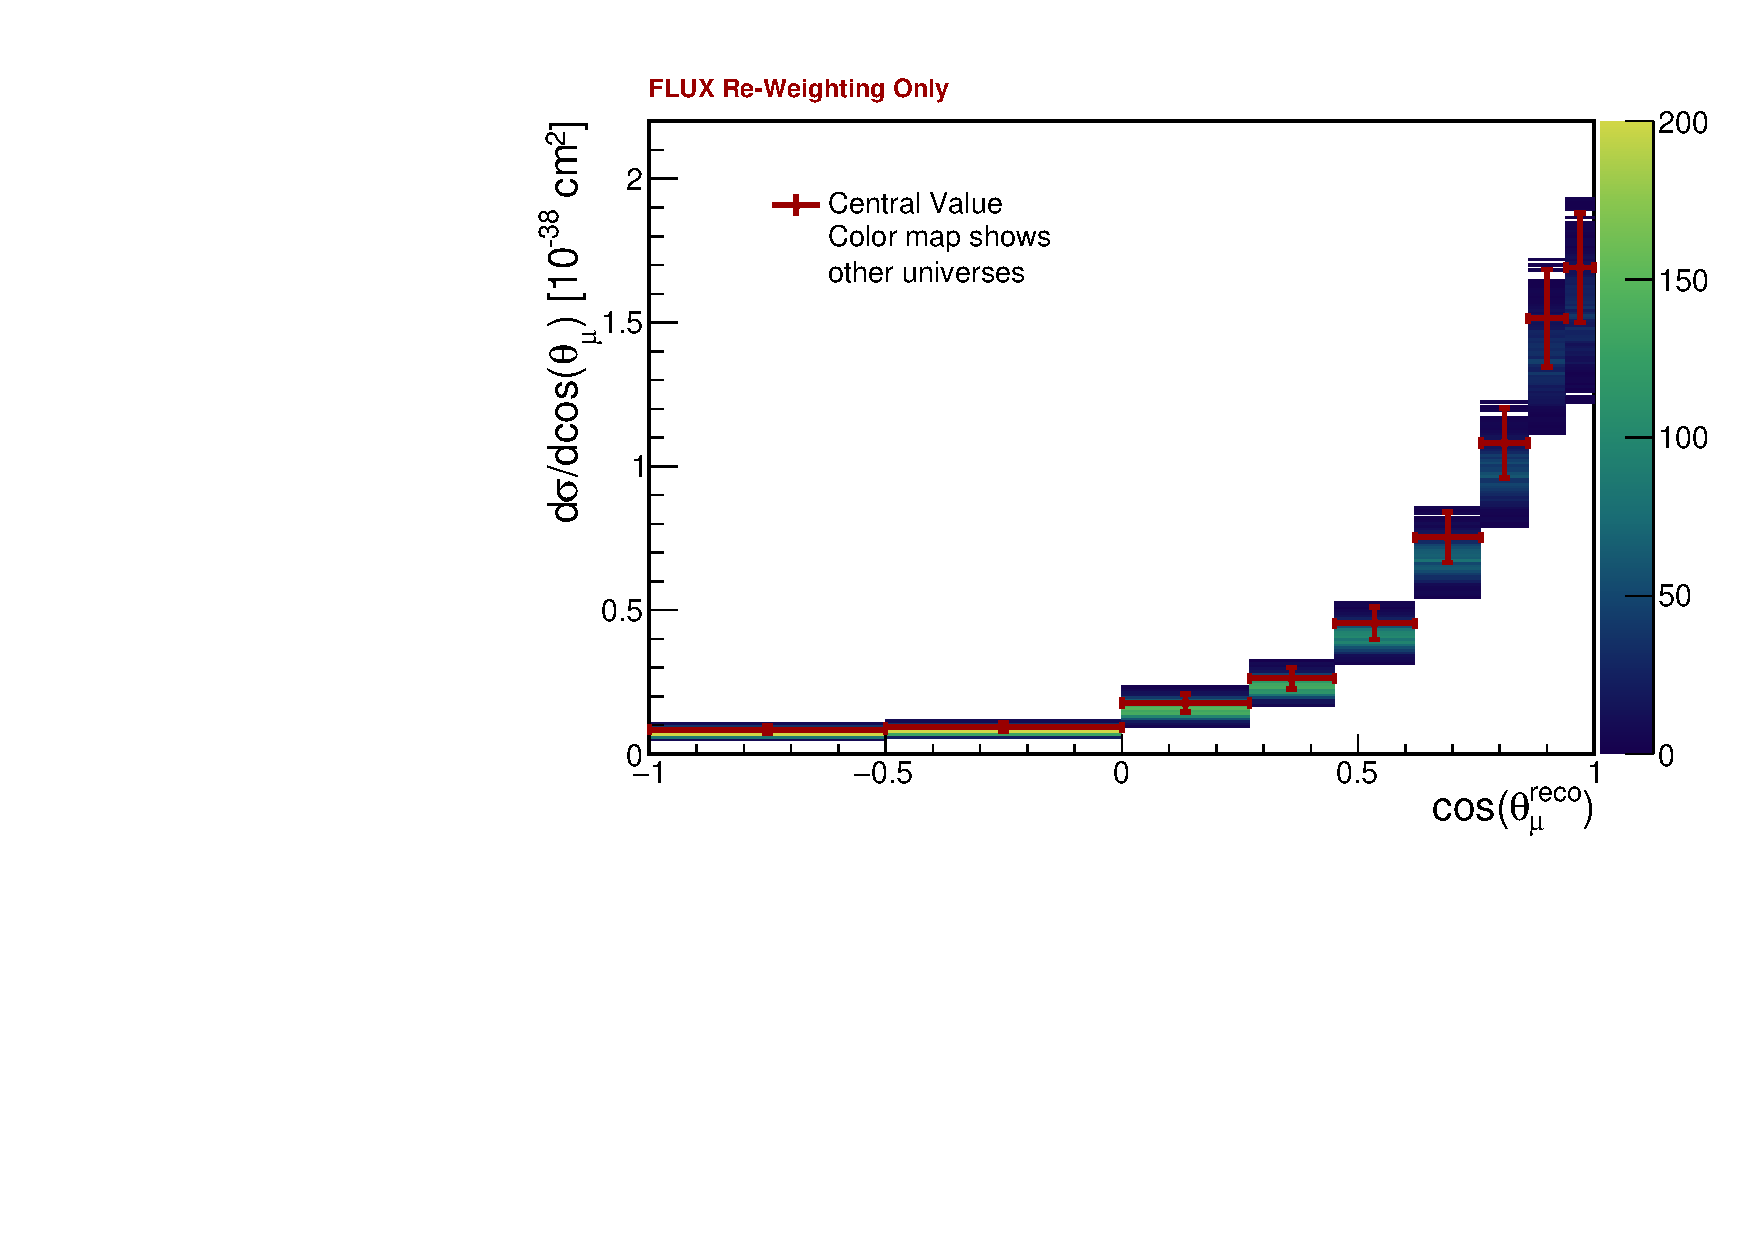
\includegraphics[width=.5\textwidth]{images/flux_covariance_plots/flux_multisim_muangle_xsec_all_fancy}
   \label{fig:flux_multisim_muangle_xsec_all_fancy}} 
\caption[Beam Flux Uncertainties - Single-Differential Cross Sections - Universes Distributions]{\emph{Beam Flux Uncertainties.} 
Data extracted differential cross sections in muon momentum~\protect\subref{fig:flux_multisim_mumom_xsec_all_fancy} and cosine of the muon angle~\protect\subref{fig:flux_multisim_muangle_xsec_all_fancy} for all simulated universes in the colour map. Only flux variations are included in these plots. The red graph shows the data extracted cross section for the nominal \acrshort{mc}. The red vertical bars show the uncertainties derived from the \emph{multisims} according to Equation~\eqref{eq:cov_syst_uni}.}
\label{fig:flux_multisim}
%\end{adjustwidth}
\end{figure}







\clearpage
%**********************************************************
\section{Detector Uncertainties}
\label{sec:error_detector}

In this section, the detector-related systematic uncertainties are described. While the understanding of the \acrshort{lartpc} detectors have been improved significantly in the past few years, there are still areas where further refinements in the simulation are required. At this point, conservative estimates of the possible systematic biases in the MicroBooNE simulation are made, and are treated as symmetric $1\sigma$ uncertainties.
The detector systematic uncertainties are evaluated via \emph{unisims} and Equation~\eqref{eq:syst_det} is used to calculate the covariance matrix. Variation samples for a set of 13 detector parameters have been generated. Variations of the central value were created by using a $\pm1\sigma$ range for parameters where constraints from data were available, or otherwise by simulating an alternative model. The list of parameters is given in Table~\ref{tab:det_syst}.
Work is currently ongoing to improve the knowledge on proper uncertainty ranges and detector systematics uncertainties are expected to be improved in the next iteration of this analysis.
The uncertainty on the total cross section related to the above-listed detector effects has been calculated and the covariance matrices are shown in Figure~\ref{fig:cov_det} and~\ref{fig:cov_det_muangle_mumom}. Here, the covariance matrix is evaluated using Equation~\ref{eq:syst_det}. 
 The relative detector systematic uncertainty on the total cross section currently amounts to 16\%. Contributions of individual effects are listed in Table~\ref{tab:det_syst}. For parameters with both plus and minus $1\sigma$ variations, the larger of the relative deviations from the central value cross section is chosen as an uncertainty to use in the total uncertainty budget. The largest effect is due to the simulation of induced charge on neighbouring wires. 


\begin{table}[]
\begin{adjustwidth}{-1cm}{-1cm}
\centering%
\caption[Detector Modelling Systematic Uncertainties]{List of parameters varied for the detector systematic studies.}
\label{tab:det_syst}
\newcolumntype{A}{>{\hsize=0.8\hsize}X}
\newcolumntype{B}{>{\hsize=0.6\hsize}X}
\newcolumntype{Y}{>{\hsize=2.1\hsize}X}
\newcolumntype{Z}{>{\hsize=.5\hsize}X}
\begin{tabularx}{\linewidth}{AYZB}
\toprule
Detector Systematic Sample              & Description     & Type & Total Cross Section Relative Uncertainty [\%]\\
\midrule
Space Charge                  &  A simple data-driven calibration is applied to the space charge simulation to make it better match measured space charge effects \cite{space_charge}.  & Modified Model   & 3.7  \\
Induced Charge                &  Charge induction is simulated on a longer spatial range than in the default \acrshort{mc}, so that more distant wires see the effect of drifting charge. & Alternate Model   & 13\\
Light Yield                   &  An improved light production simulation model is used.  & Alternate Model  &  4.7 \\
Remove Channels Prone to Saturating         &   Turning off channels that frequently become saturated as charge builds up on capacitors in the ASIC circuits, resulting in deadtime.  &   Alternate Model & 4.3 \\
Remove Misconfigured Channels     &  Turning off the misconfigured channels associated with ASICs that have a different gain and shaping time than desired & Modified Model & 1.8 \\
Wire Response Function        &  The wire response functions used during deconvolution are stretched by 20\% based on MicroBooNE data. & $\pm1\sigma$ & 0.25 \\
Longitudinal Diffusion        &  The amplitude of longitudinal diffusion is varied based on world data \cite{Li:2015rqa, Cennini:1994ha}.    & $\pm1\sigma$ & 1.7 \\
Transverse Diffusion          &  The amplitude of transverse diffusion is varied based on world data \cite{TD01, TD02, TD03}.   & $\pm1\sigma$ & 1.6 \\
Wire Noise                    &  The amplitude of the wire noise model varied. & $\pm1\sigma$ & 0.089 \\
\acrshort{pe} Noise                      &  The single-\acrshort{pe} noise of the \acrshort{pmt}s is varied.  & $\pm1\sigma$ & 0.38 \\
\acrshort{tpc} Visibility                &  The light yield in the cryostat but outside the \acrshort{tpc} is increased by 50\%.  & Alternate Model & 3.7 \\
Electron Lifetime             &  The electron lifetime is reduced to 10 ms. (This condition affects only about $\sim$10\% of data taken with lower purity). & Alternate Model &  2.9 \\
Electron Recombination        &  The Birks recombination model, with parameters derived from ICARUS~\cite{birks_icarus}, is used instead of the default modified box model, with parameters derived from ArgoNeuT~\cite{birks_argoneut}.  & Alternate Model & 0.060 \\
\midrule
\multicolumn{3}{l}{Total combined relative uncertainty} & 16\\
\bottomrule
\end{tabularx}
\end{adjustwidth}
\end{table}


The following points describe why some effect produce a large cross-section variation, and discuss on future improvements:
\begin{itemize}
\item \emph{Induced-Charge Effect.} A charge is induced on neighbouring wires when electrons provoke a signal on an induction plane wire, or are deposited on a collection plane wire. In the simulated sample that includes the induced-charge effect, the 13\% cross section difference comes from a change in the number of selected signal events that affect the efficiency in Equation~\eqref{eq:xsec_total}. In this simulation there are less reconstructed neutrino-induced muons at the Pandora stage before any selection takes place. This effect is currently being implemented and will be included in the default simulation with a reasonable parameter range of variation, with an expected significant reduction of its effect on the measurement.
\item \emph{Space-Charge Effect.} Space charge refers to the presence of positively charged ions that are formed when the argon is ionised. These ions influence the recombination of ionisation electrons from new interactions, and can cause distortions in the readout. In the simulated sample where the space charge effect is decreased, the main difference with respect to the nominal simulation arises in the number of \acrshort{outfv} background events being selected. There are less \acrshort{outfv} selected events in the variation sample. In the nominal simulation, many events happening outside the \acrshort{fv} are pushed in the \acrshort{fv} by space-charge distortion, and appear as \acrshort{outfv} background. The number of such events decreases if the space charge is turned off.  
\item \emph{Light Yield, Saturating and Misconfigured Channels, \acrshort{tpc} Visibility and Electron Lifetime.} All these effect, that produce an uncertainty of the order of ~4\%, will decrease in a future iteration of this analysis, when a more data-driven model of the detector will be available. This is achieved by overlaying beam-off data, and the \g neutrino simulation, without the need to simulate the \acrshort{cr} background.
\end{itemize}


%The relative detector systematic uncertainty on the total cross section amounts to 16.2\%.

\begin{figure}[t]
%\begin{adjustwidth}{-1cm}{-1cm}
\centering
\subfloat[][Covariance matrix for $p_\mu$.]
   {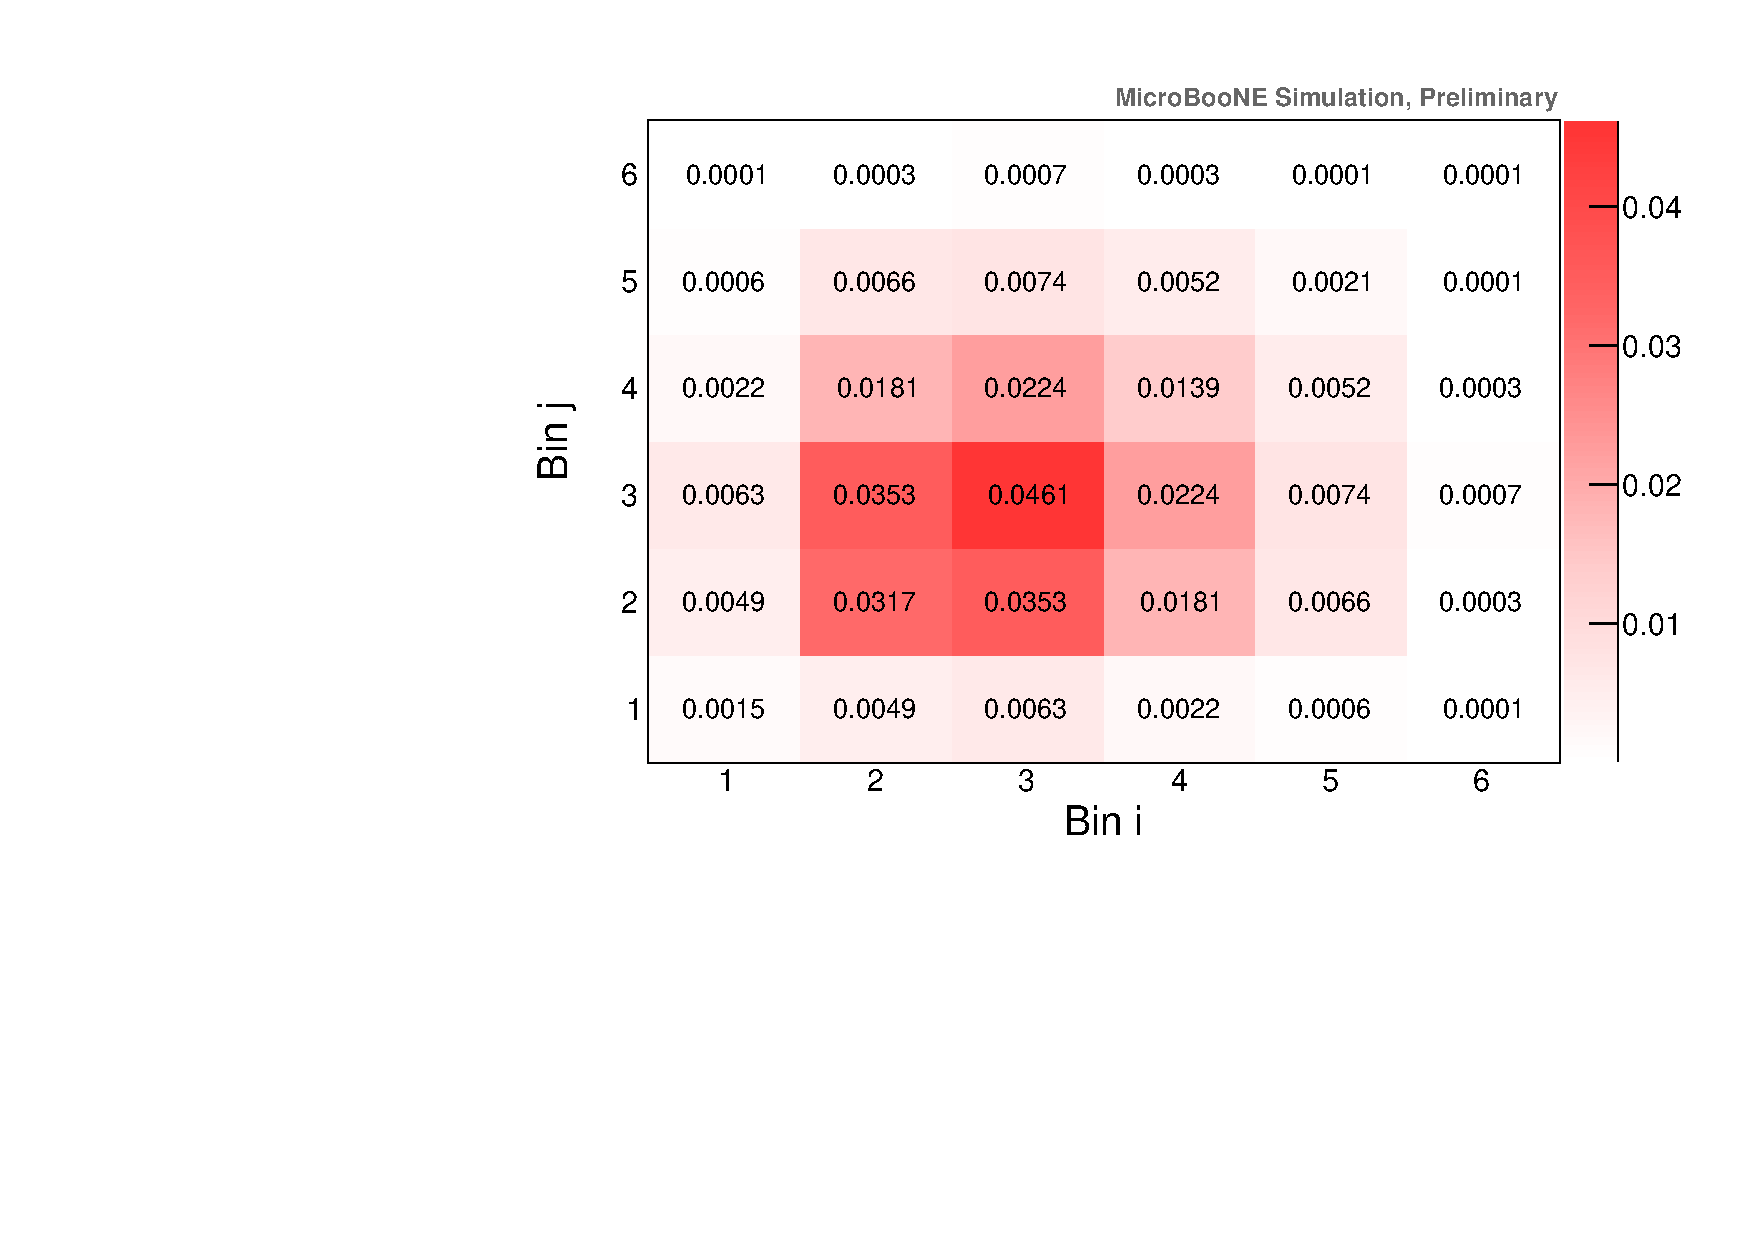
\includegraphics[width=.5\textwidth]{images/detector_covariance_plots/cov_det_mumom}
   \label{fig:cov_det_mumom}} 
\subfloat[][Covariance matrix for $\cos\theta_\mu$.]
   {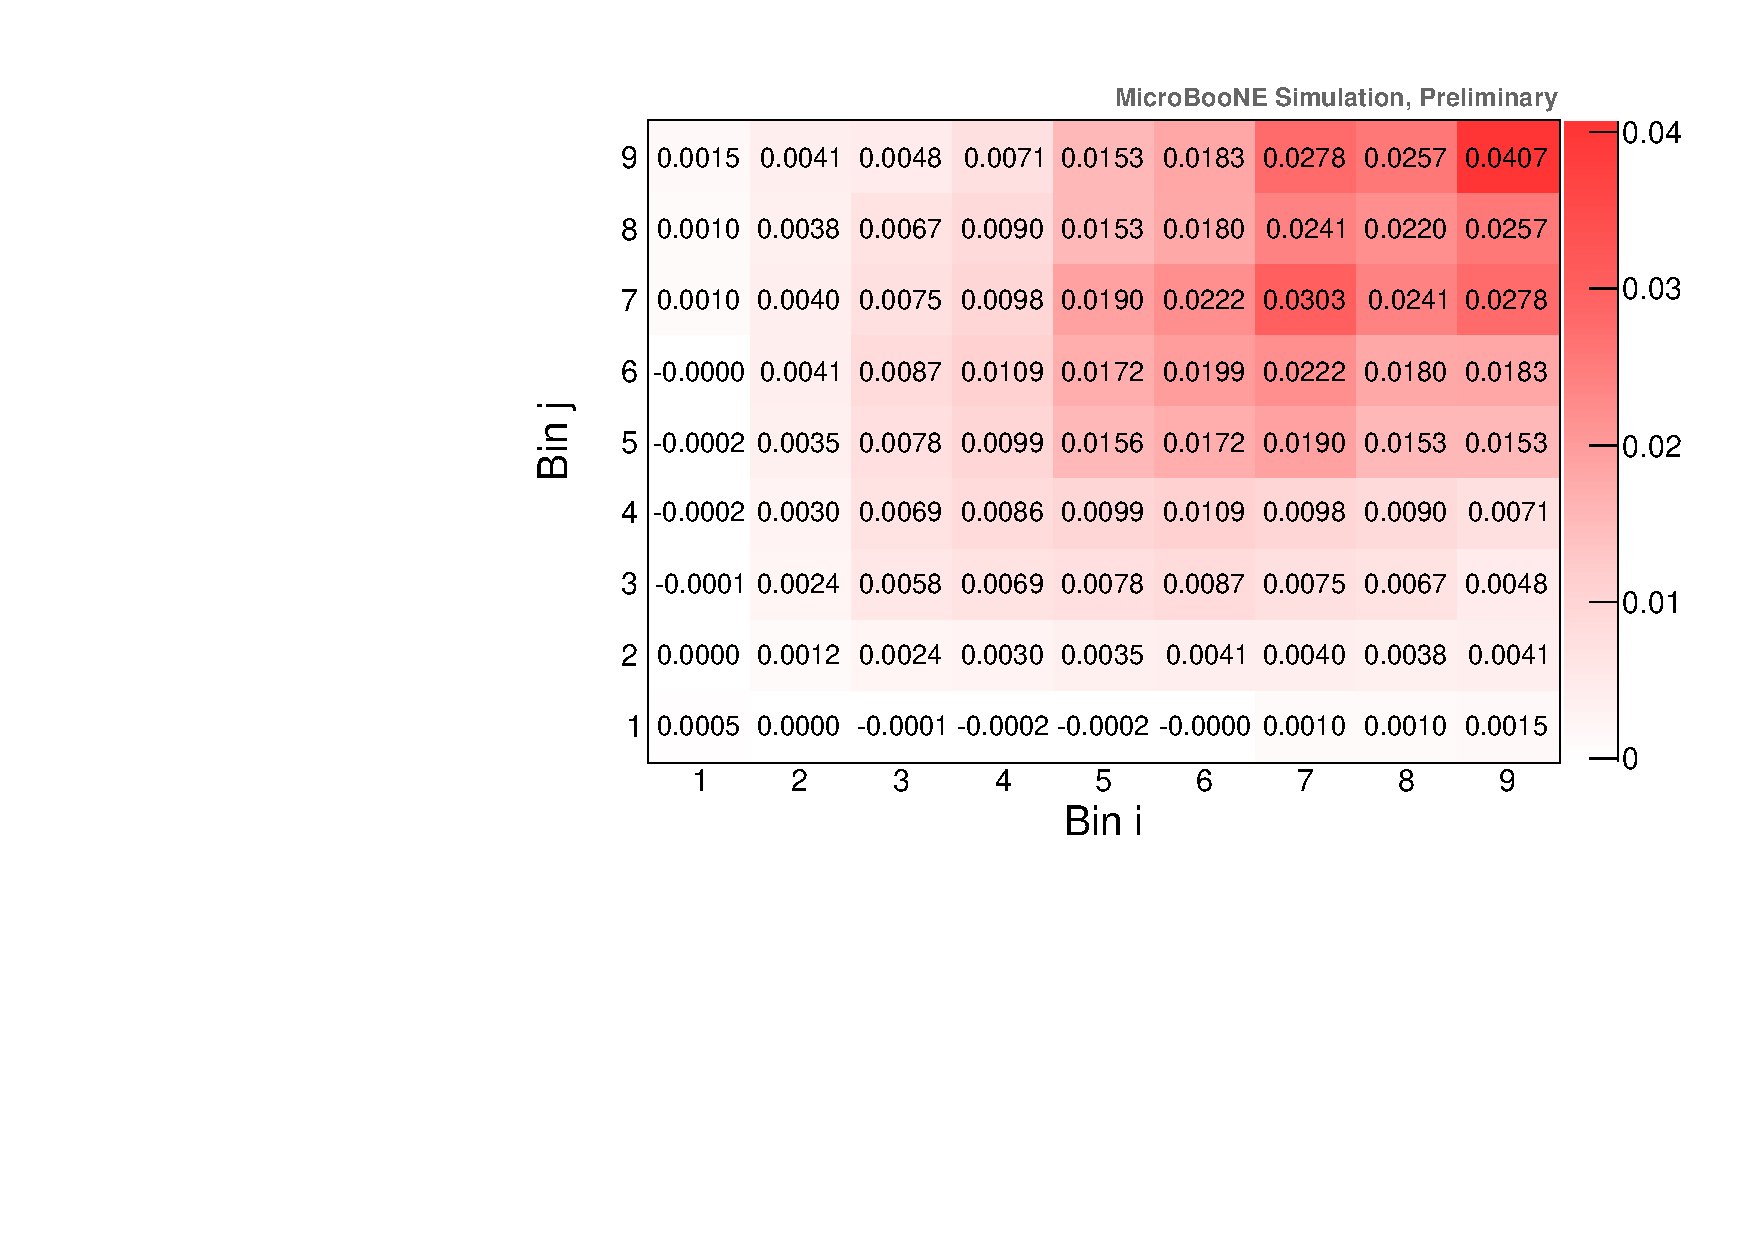
\includegraphics[width=.5\textwidth]{images/detector_covariance_plots/cov_det_muangle}
   \label{fig:cov_det_muangle}} \\
\subfloat[][Fractional covariance matrix for $p_\mu$.]
   {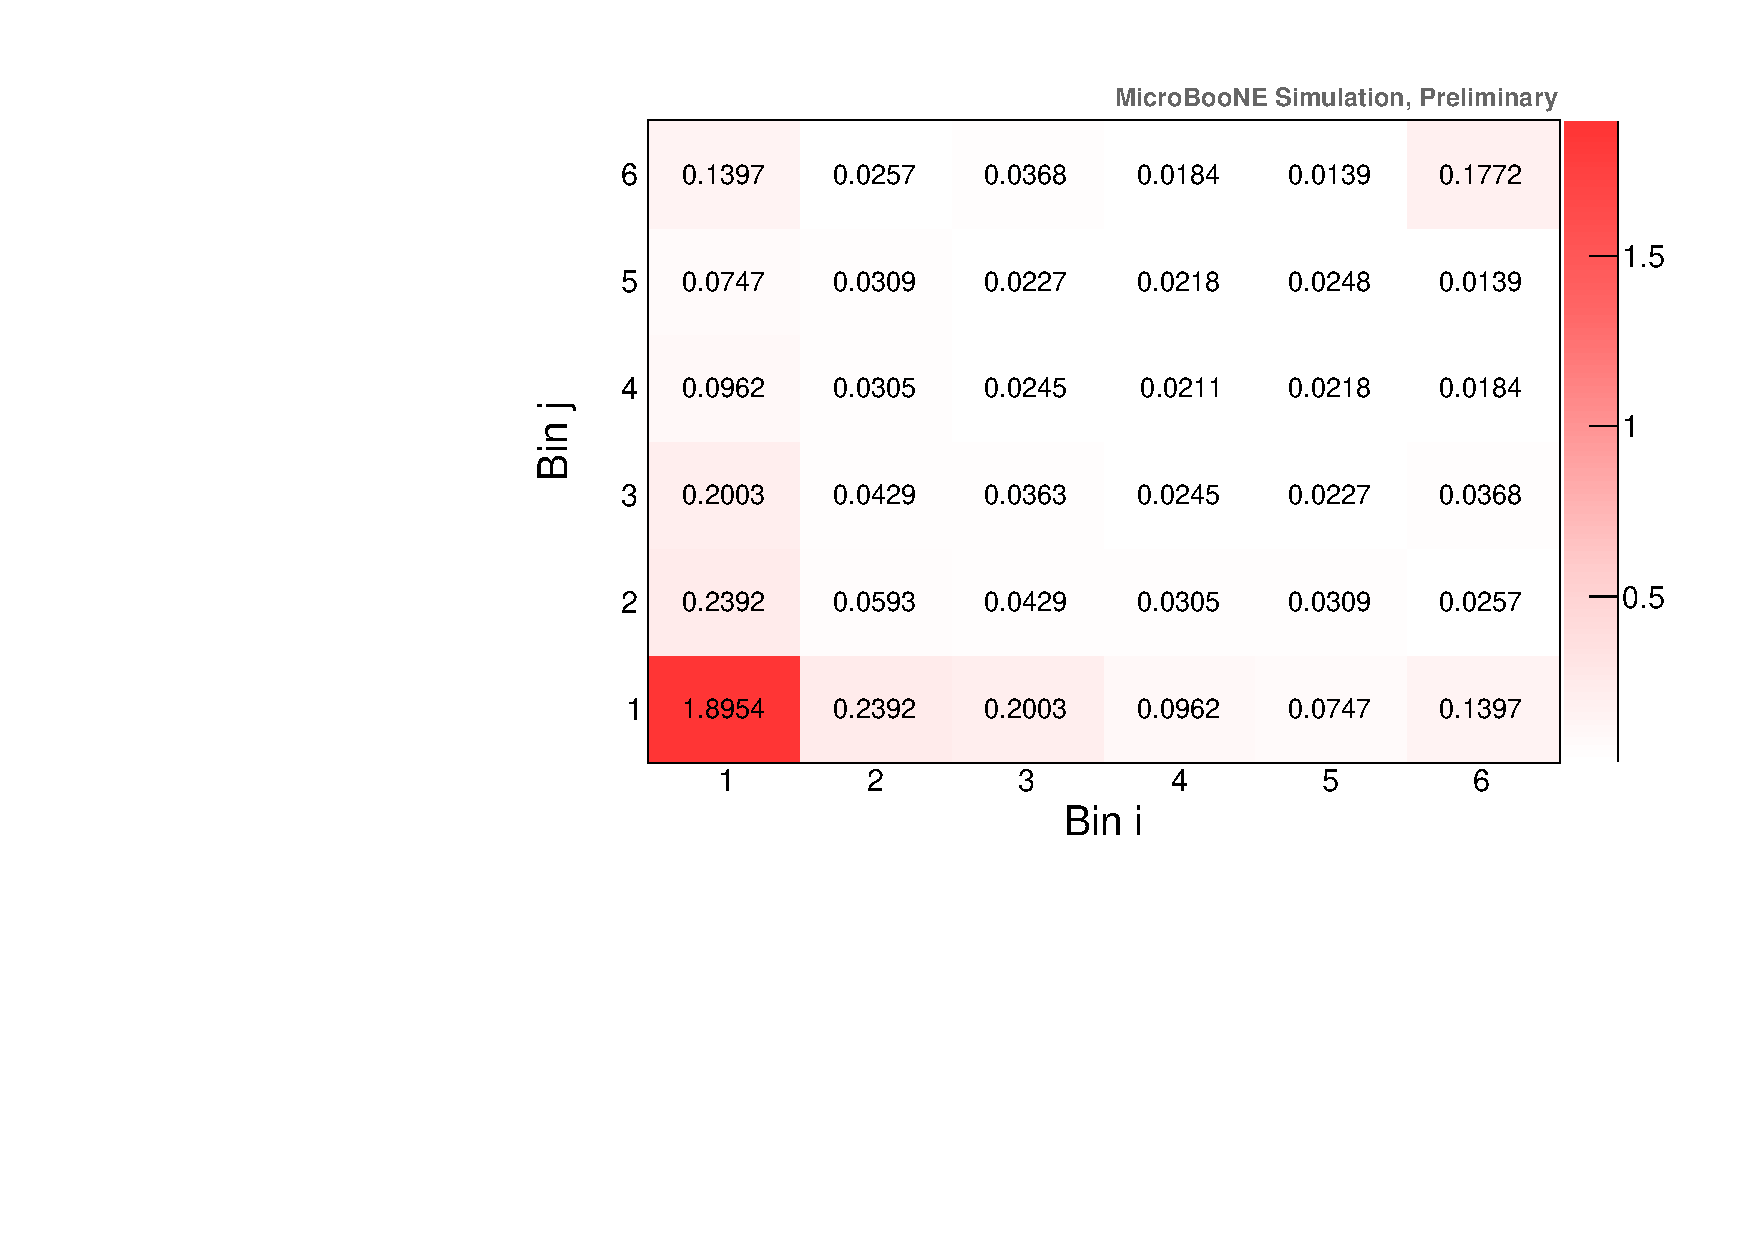
\includegraphics[width=.5\textwidth]{images/detector_covariance_plots/cov_det_frac_mumom}
   \label{fig:cov_det_frac_mumom}} 
\subfloat[][Fractional covariance matrix for $\cos\theta_\mu$.]
   {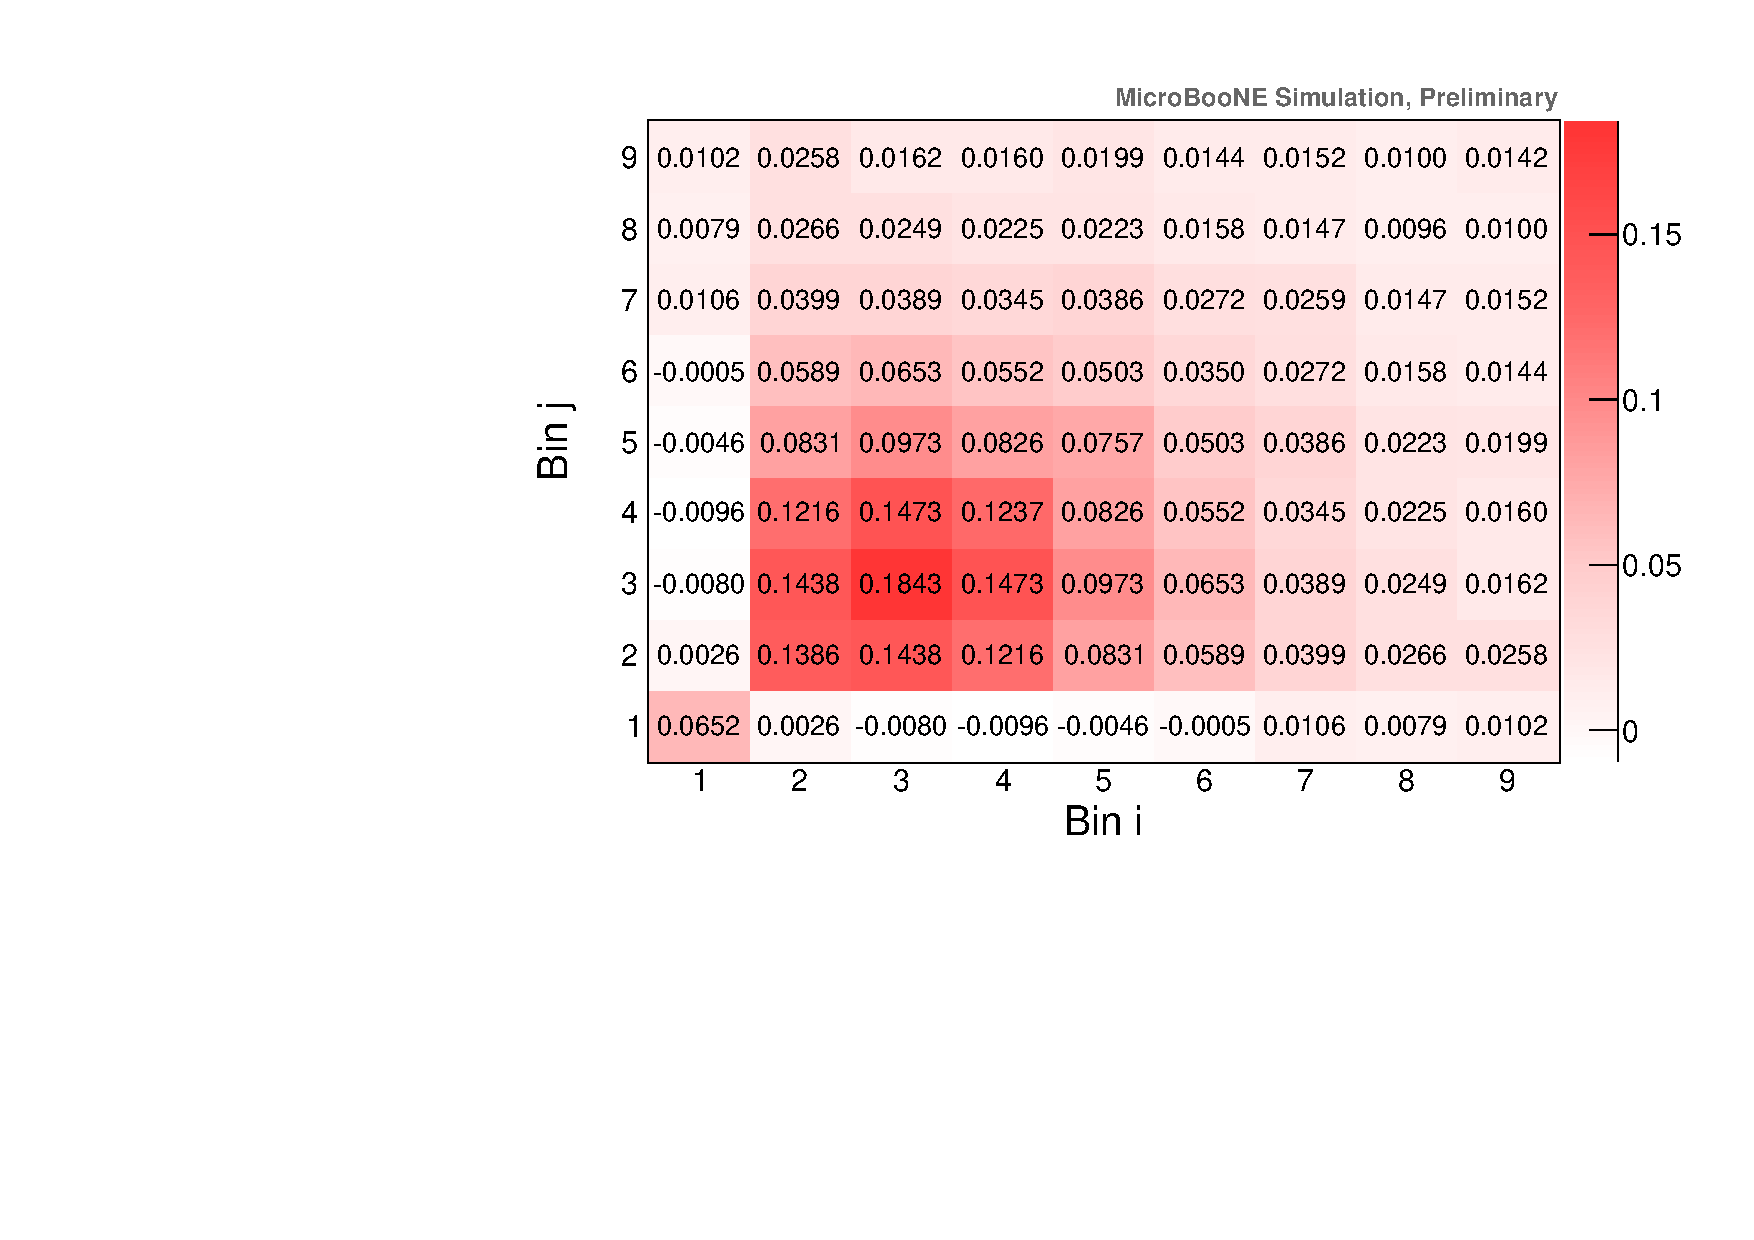
\includegraphics[width=.5\textwidth]{images/detector_covariance_plots/cov_det_frac_muangle}
   \label{fig:cov_det_frac_muangle}} \\
\caption[Detector Response Uncertainties - Single-Differential Cross Sections - Covariance Matrices]{\emph{Detector Response Uncertainties.} The detector response systematic covariance matrices for muon momentum~\protect\subref{fig:cov_det_mumom} and muon angle~\protect\subref{fig:cov_det_muangle} bins, respectively and the fractional covariance matrices for muon momentum~\protect\subref{fig:cov_det_frac_mumom} and muon angle~\protect\subref{fig:cov_det_frac_muangle} bins, respectively.}
\label{fig:cov_det}
%\end{adjustwidth}
\end{figure}



\begin{figure}[]
\centering
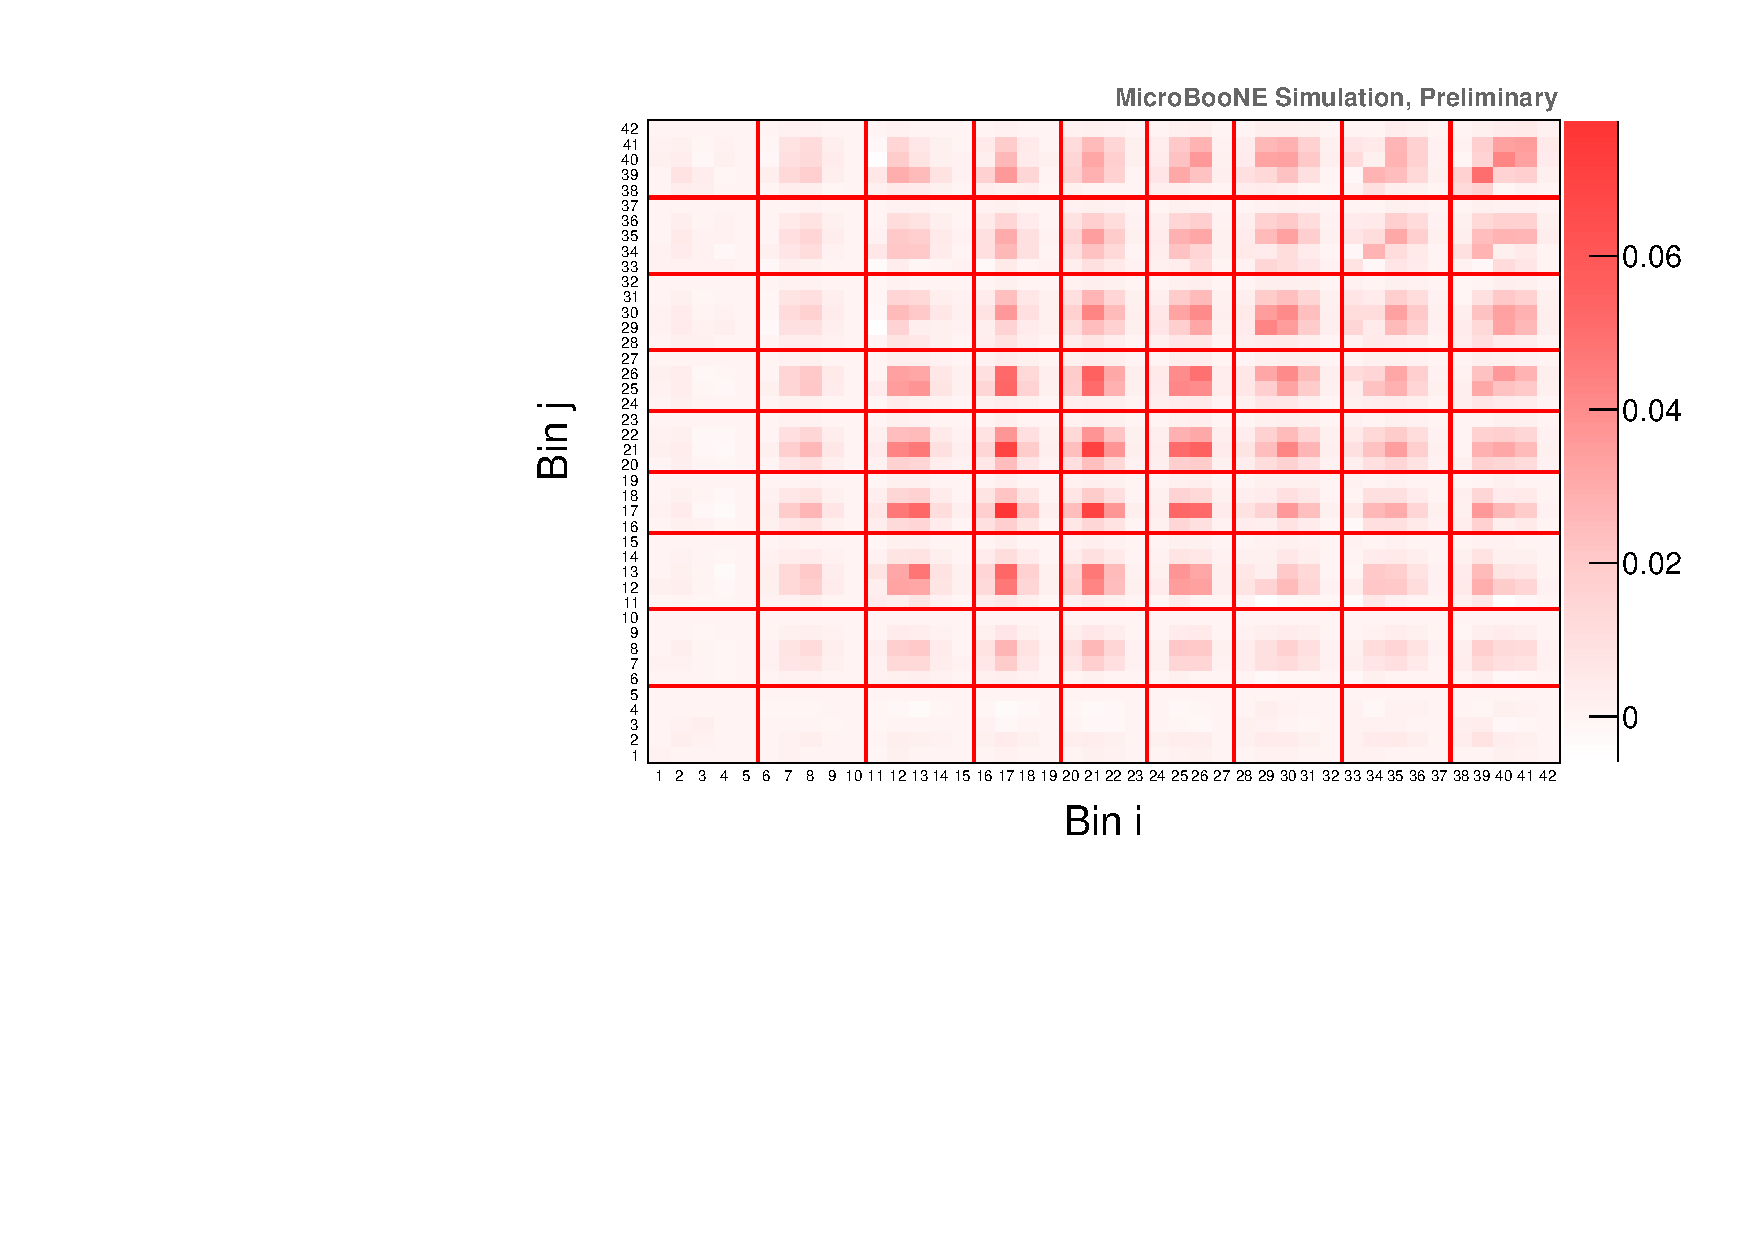
\includegraphics[width=.80\textwidth]{images/detector_covariance_plots/cov_det_muangle_mumom}
\caption[Detector Response Uncertainties - Double-Differential Cross Section - Covariance Matrix]{\emph{Detector Response Uncertainties.} Covariance matrix for the double-differential cross section. Only detector variations are included.}
\label{fig:cov_det_muangle_mumom}
\end{figure}







\subsection{Uncertainty on the Number of Targets}
\label{sec:error_targets}

The two contributors to a potential variation on the calculated number of targets are argon density and \acrshort{fv}. To understand the uncertainty on the density, the temperature and pressure of the detector during the period in which the data was taken must be considered. These values are extracted from sensors in the detector and the cryogenic system. During the beam-on data taking, temperature and pressure were measured to be $89.2 \pm 0.3$ K and $1.241 \pm 0.004$ bar, respectively. Accounting for variations of these values, the liquid argon density with its uncertainty is $1.3836^{+0.0019}_{-0.0002}$ g/cm$^3$: it is a 0.1\% effect. This effect is safely negligible considering the size of the other uncertainties currently taken into account.



\section[Uncertainty on Simulated Cosmics]{Uncertainty on the Simulated Cosmogenic Background}
\label{sec:error_cosmic}

This section addresses the uncertainty with the simulated \acrshort{cr} background. To understand the systematic associated with this background, the full analysis was run over a sample of \acrshort{bnb} simulated neutrinos overlaid with \acrshort{cr} from data, here called the ``overlay'' sample. This is different with respect to the nominal MicroBooNE simulation, where \acrshort{cr} are also simulated using \textsc{Corsika} (see Section~\ref{sec:simulation}). The event distributions of the selected events obtained from this new sample are then compared with the nominal distributions, in order to estimate an additional systematic uncertainty. Figure~\ref{fig:overlay} shows the distribution of the muon track length and $\phi$ angle, obtained with the ``overlay'' samples. 
An overall agreement except in the bins that have a relevant \acrshort{cr} background contribution is observable. 
A scaling factor is estimated and applied to the \acrshort{cr} background only, such that the ratio between the nominal and the ``overlay'' simulations corresponds to unity in every bin. The measured scaling factor is 0.60. To estimate what impact this may have on the total cross section, this scaling factor is applied to the simulated \acrshort{cr} cosmic background, and a new cross section is extracted with this scaling applied. The difference between this new cross section and the nominal cross section is taken as an additional systematic uncertainty of the cross-section measurement. 
The relative uncertainty on the total cross section due to the simulated cosmogenic background amounts to 4.1\%.




\begin{figure}[t]
\centering
\subfloat[][]
   {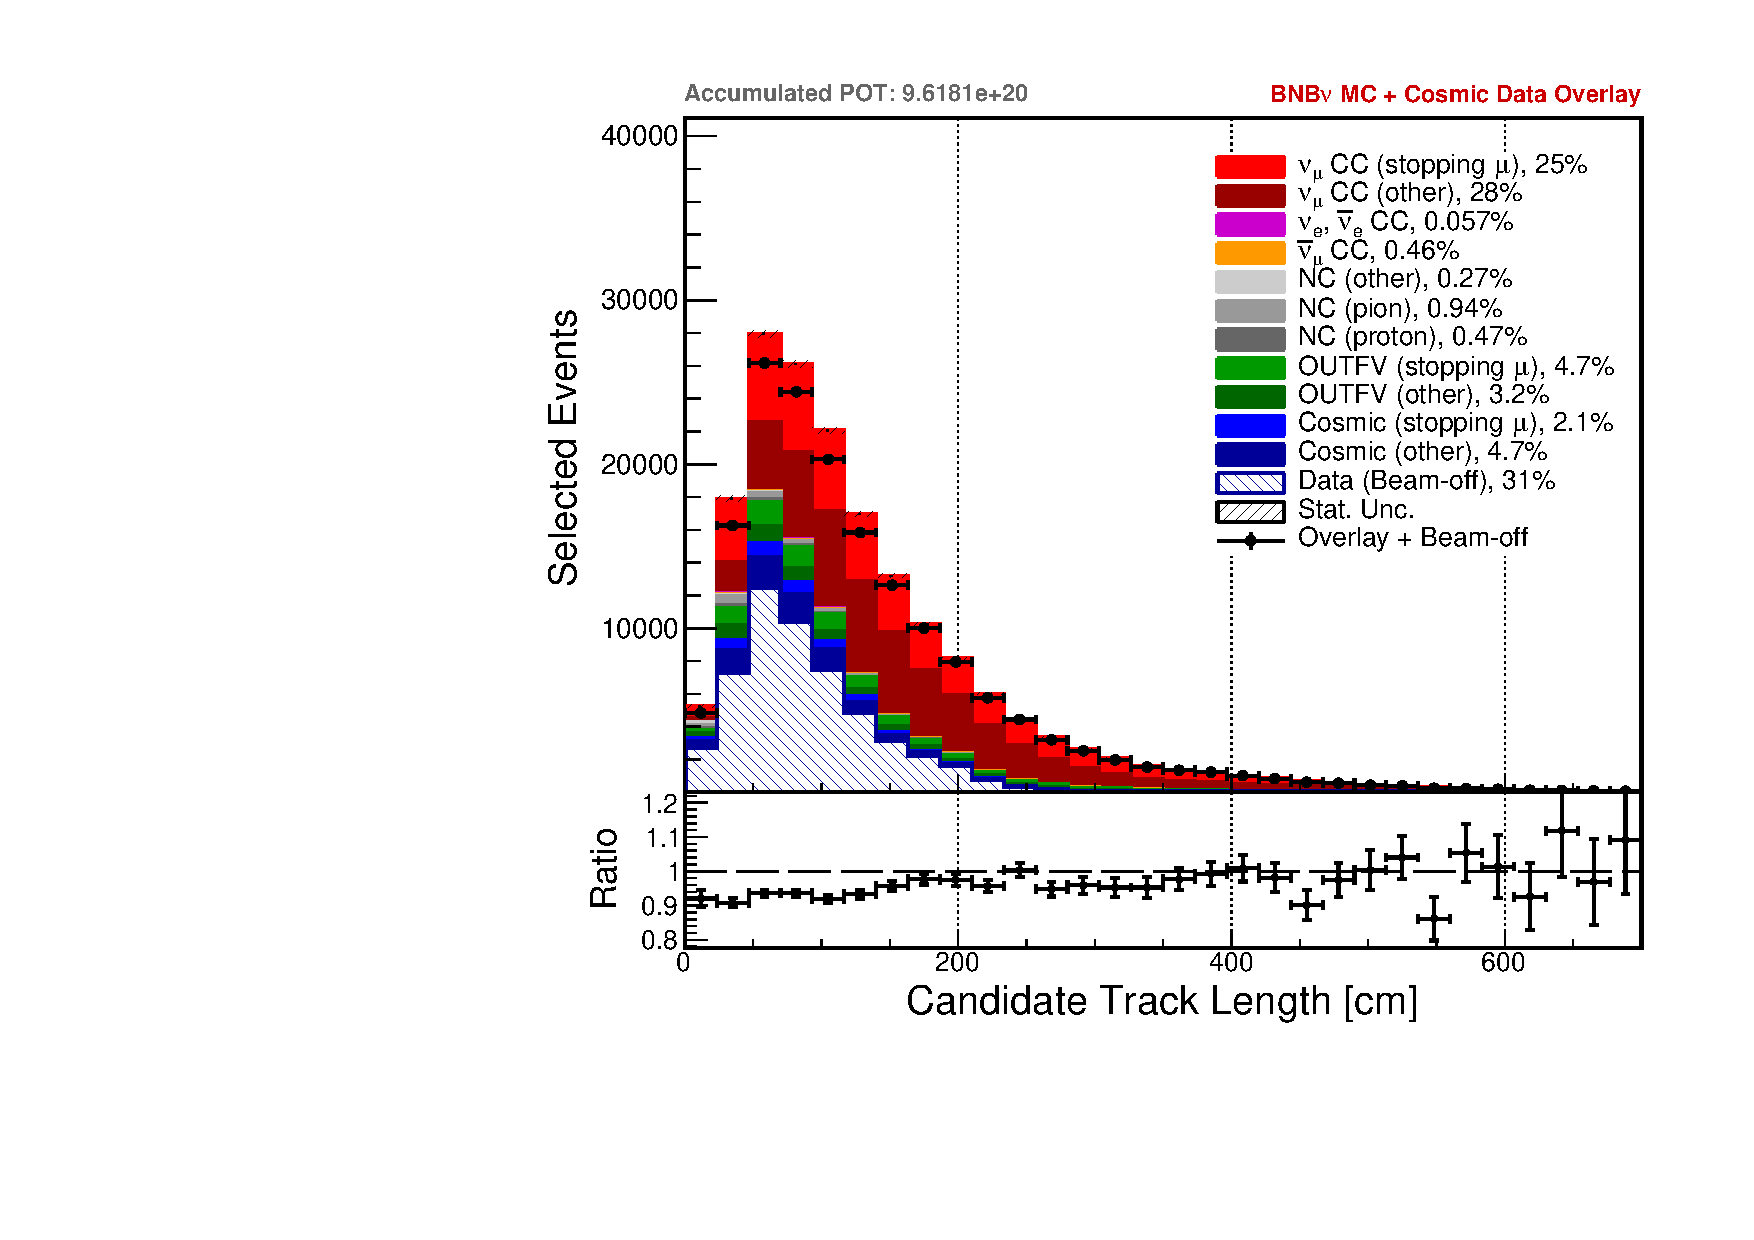
\includegraphics[width=.5\textwidth]{images/OverlayPlots/trklen_overlay}
   \label{fig:overlay_len}} 
\subfloat[][]
   {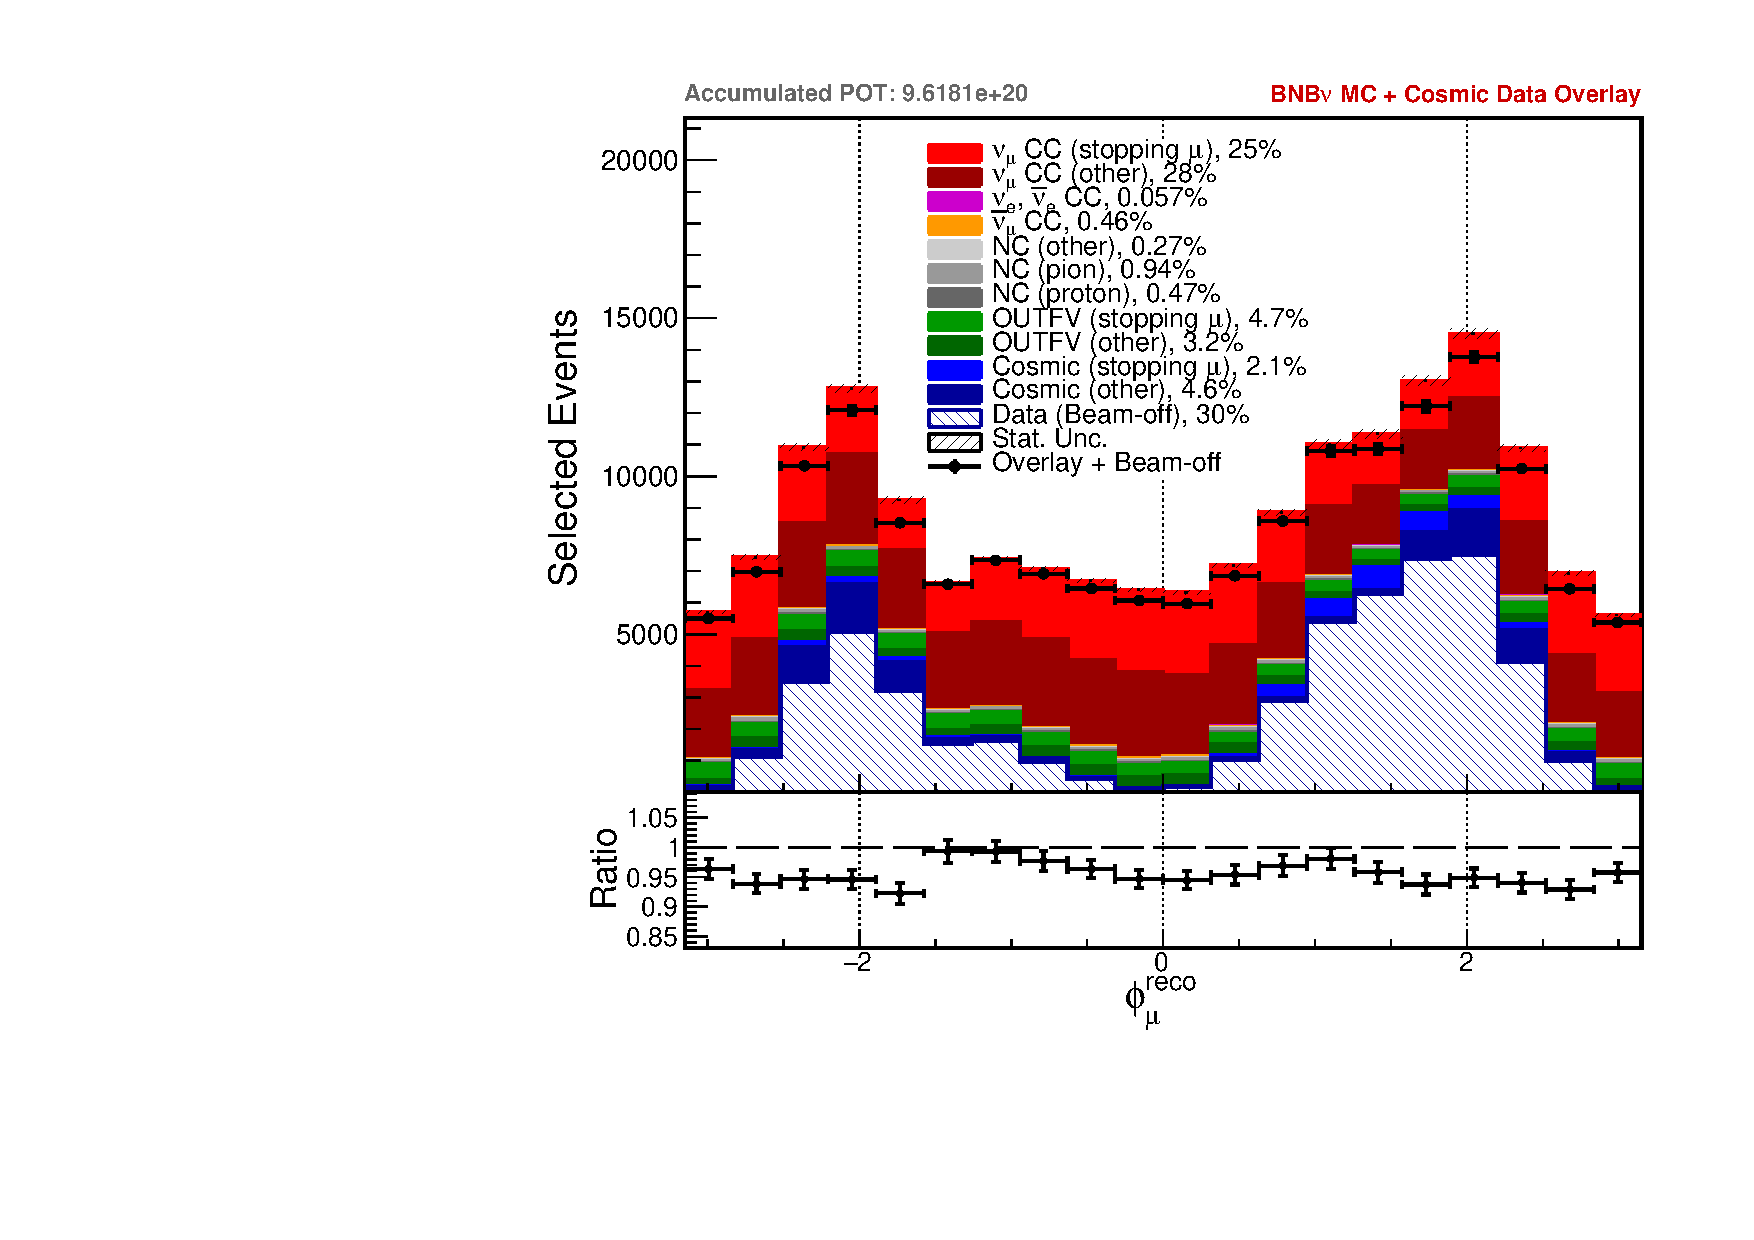
\includegraphics[width=.5\textwidth]{images/OverlayPlots/trkphi_overlay}
   \label{fig:overlay_phi}} 
\caption[Selected Event Distributions with Simulated Neutrino and Data Cosmics Overlaid]{Distributions of candidate muon track length~\protect\subref{fig:overlay_len} and $\phi$ angle~\protect\subref{fig:overlay_phi} for selected events. The black points are not from data, but come from the ``overlay'' sample. The coloured histograms show simulated events according to the nominal MicroBooNE simulation. There is good agreement between the two \acrshort{mc} samples, except in the regions were there are more \acrshort{cr} in \acrshort{bnb} background events (blue). This difference is used to estimated the systematic uncertainty due to the simulated cosmogenic background.}
\label{fig:overlay}
\end{figure}










\clearpage
\section[Uncertainty on Simulated Dirt]{Uncertainty on the Simulated Dirt Background}
\label{sec:error_dirt}


The dirt background is used to estimate events where neutrinos interact outside of the cryostat, and either a \acrshort{cr} or a neutrino-induced track entering the \acrshort{tpc} is selected. Due to the many unknowns in generating this background, that strongly depends on the building geometry, the dirt composition and the ability of \g in simulating interactions with the dirt, the MicroBooNE collaboration agreed to assign a 100\% systematic uncertainty on this sample.
%The fractional covariance matrices can be seen in Figure~\ref{fig:cov_dirt}.




\section{MC Statistical Uncertainties}
\label{sec:error_mcstat}

This section describes how the \acrshort{mc} statistical uncertainties are estimated. \acrshort{mc} statistical uncertainties are considered as an additional systematic uncertainty. The cross section is evaluated as:
\[
\left ( \frac{d\sigma}{dx_\mu} \right )_i = \frac{N_i - B_i}{ \tilde{\epsilon}_i \cdot T \cdot \Phi_{\nu_\mu} \cdot (\Delta x_\mu)_i}, \qquad \tilde{\epsilon}_i = \frac{\sum_jS_{ij}N_j^\text{sel}}{\sum_jS_{ij}N_j^\text{gen}},
\]
and similarly for the double-differential cross section.
Since the same \acrshort{mc} sample is used to evaluate $N_j^\text{gen}$, $N_j^\text{sel}$ and $S_{ij}$, it is then not possible to propagate statistical uncertainties as if those quantities were independent. The smearing matrix $S$ makes it hard to analytically propagate the statistical uncertainties. 

For this reason, a \emph{multisim} approach was followed for the \acrshort{mc} statistical uncertainties. The idea is to generate Poisson random numbers for each event, and for several universes, and to extract the cross section for every universe. The distribution of cross sections for every universe will then give an estimation for the \acrshort{mc} statistical uncertainties. All possible correlations introduced by using the same events for $N_j^\text{gen}$, $N_j^\text{sel}$ and $S_{ij}$ will be automatically taken into account by this method. This method is also referred to as the ``bootstrap method''~\cite{bootstrap}.

In the bootstrap method, toy \acrshort{mc} samples are drawn for each event. Poisson random numbers are generated with $\mu = 1$ such that the average over bootstrap replicas for a given event yields one event. The weights are integer numbers, such that each event can be taken 0, 1, 2, \dots $N$ times. 
%The bootstrap weights can be generated uniquely for all input events, as they can be seeded by the run, subrun and event numbers. 
The fractional covariance matrix is shown in Figure~\ref{fig:mc_stat_multisim_muangle_mumom_cov_matrix_2d}, and relative uncertainty on the total cross section amounts to 0.2\%

\begin{figure}[]
\centering
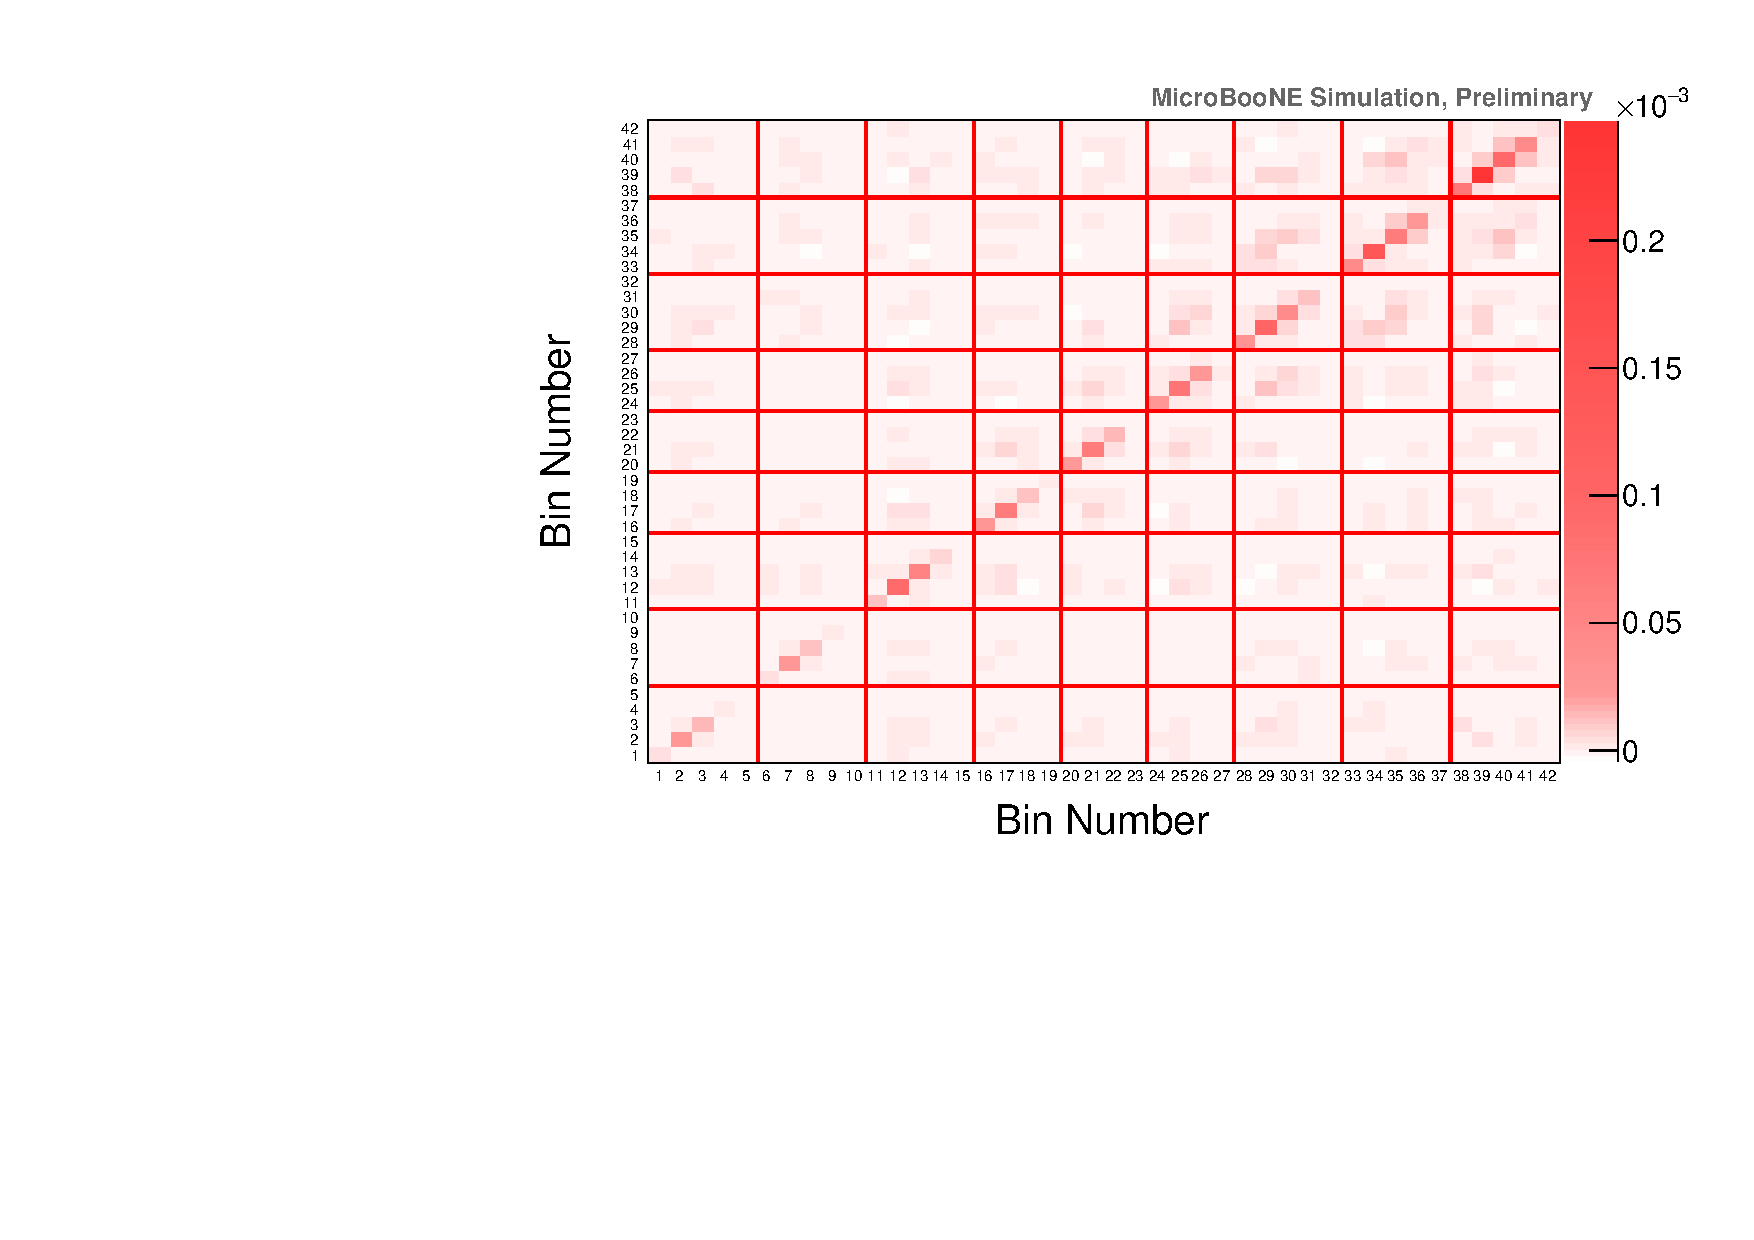
\includegraphics[width=.80\textwidth]{images/mc_stat_covariance_plots/mc_stat_multisim_muangle_mumom_cov_matrix_2d}
\caption[\acrshort{mc} Statistical Systematic Uncertainties]{\emph{\acrshort{mc} Statistical Uncertainties.} \acrshort{mc} statistics fractional covariance matrix, for the double differential cross section.}
\label{fig:mc_stat_multisim_muangle_mumom_cov_matrix_2d}
\end{figure}


\clearpage
%**********************************************************
\section{Systematic Uncertainties Summary}
\label{sec:syst_unc_summary}

This chapter has described the estimation and implementation of the systematic uncertainties that affect the $\nu_\mu$ \acrshort{cc} inclusive cross-section measurement. The systematic uncertainties due to cross-section modelling and flux have been estimated using a \emph{multisim} approach, where several universes have been generated, and the cross section was extracted for every universe. The variance of this distribution gives the systematic uncertainty on the cross section, which amounts to 3.6\% for the cross-section modelling and 12.2\% for the beam flux modelling.
For the systematic uncertainties coming from the detector simulation, a \emph{unisim} approach was used instead, where an \acrshort{mc} sample was generated for each single detector parameter variation. The difference between the nominal cross section and the cross section obtained in each of these \acrshort{mc} runs is the estimation for the detector systematic uncertainty. The estimated systematic uncertainty amounts to 16.2\%, dominated by the induced charge effect (13\%).
Other systematic uncertainties arise from \acrshort{cc}\acrshort{qe} and \acrshort{cc}\acrshort{mec} uncertainties (1.4\%), particle re-interaction uncertainties (0.6\%), the \acrshort{pot} counting (2\%), the simulated cosmic background (4\%), the dirt background (11\%) and the \acrshort{mc} statistics (0.2\%). These are summarised in Table~\ref{tab:all_syst}. The total systematic uncertainty, obtained by summing all the mentioned uncertainties in quadrature, adds up to 23.8\%.
The next chapter will show the cross section with both statistical and systematic uncertainties.

%\begin{table}[]
%\begin{adjustwidth}{-1.3cm}{-1.3cm}
%\centering
%\caption[Summary of Systematic Uncertainties]{The table shows the different contributions to the total cross section systematic uncertainty.}
%\label{tab:all_syst}
%\begin{tabular}{c l c}
%\toprule
%Uncertainty Source        & Method & Estimated Relative     \\
%                          &        & Uncertainty     \\
%\midrule
%Beam Flux                 &  Estimated with multisim variations &  12.2\%       \\
%Cross Section Modelling   &  Estimated with multisim variations &  3.55\%        \\
%\acrshort{cc}QE/\acrshort{cc}MEC                &  Estimated with multisim variations &  1.44\%        \\
%Particle Re-Interaction   &  Estimated with multisim variations &  0.612\%        \\
%Detector Response         &  Estimated with unisim variations   &  16.2\%       \\
%POT Counting              &  Toroids Resolution                 &  2.00\%          \\
%Dirt Background           &  Estimated                          &  10.9\%        \\
%Cosmics (out-of-time)     &  Estimated from overlay sample      &  4.05\%        \\
%Cosmics (in-time)         &  Estimated from off-beam statistics &  0.743\%        \\
%\acrshort{mc} Statistics             &  Estimated with multisim variations &  0.215\%        \\
%\midrule
%Total Combined            &  -                                  &  23.8\%       \\
%\bottomrule
%\end{tabular}
%\end{adjustwidth}
%\end{table}

\begin{table}[]
%\begin{adjustwidth}{-1.3cm}{-1.3cm}
\centering
\caption[Summary of Systematic Uncertainties]{The table shows the different contributions to the total cross section systematic uncertainty.}
\label{tab:all_syst}
\begin{tabular}{c c}
\toprule
Uncertainty Source         & Estimated Relative     \\
                           & Uncertainty     \\
\midrule
Beam Flux                 &  12.2\%       \\
Cross Section Modelling   &  3.6\%        \\
\acrshort{cc}\acrshort{qe} and \acrshort{cc}\acrshort{mec} Modelling               &  1.4\%        \\
Particle Re-Interaction   &  0.6\%        \\
Detector Response         &  16.2\%       \\
\acrshort{pot} Counting   &  2.0\%          \\
Dirt Background           &  10.9\%        \\
Cosmic Ray Background (\textsc{Corsika})         &  4.1\%        \\
Cosmic Ray Background (Beam-off data)     &  0.7\%        \\
\acrshort{mc} Statistics  &  0.2\%        \\
\midrule
Total Combined            &  23.8\%       \\
\bottomrule
\end{tabular}
%\end{adjustwidth}
\end{table}


